\documentclass[letterpaper,12pt]{article}

\usepackage{fullpage} % Package to use full page
\usepackage{parskip} % Package to tweak paragraph skipping
\usepackage{tikz} % Package for drawing
\usepackage{mathtools}
\usepackage[unicode]{hyperref}
\usepackage{amsfonts}
\usepackage{fancyhdr}
\usepackage{times}
\usepackage{changepage}
\usepackage{amssymb}
\usepackage{amsthm}
\usepackage{amsmath}
\usepackage[spanish,es-nodecimaldot]{babel}
\usepackage{graphicx}
\usepackage{subcaption}
\usepackage{float}
\usepackage[export]{adjustbox}
\usepackage{xcolor}
\usepackage{verbatim}

\hypersetup{
    colorlinks,
    linkcolor={blue!80!black},
    citecolor={blue!50!black},
    urlcolor={blue!80!black}
}
\theoremstyle{plain}
\newtheorem{theorem}{Theorem}

\usepackage{authblk} % Paquete para manejar autores y afiliaciones
\renewcommand\Authand{ y } % Cambiar "and" por "y"

\title{Trabajo práctico 1: Imágenes digitales} % Título del documento

%\author[1]{Ignacio Lembo Ferrari \thanks{Correo electrónico: ignacio.lembo@ib.edu.ar}}
\author[1]{Ignacio Lembo Ferrari}
\affil[1]{Instituto Balseiro}
%\affil[2]{Departamento de Física, Universidad de Ejemplo}

\date{\vspace{-4ex}}

\begin{document}

\maketitle
\section{Transformaciones de contraste \label{ej1}}

\subsection{Transformación semilinear}

Se tiene una imagen $\verb|ImagenA.pgm|$ de $181\times217$ pixels$^2$ de la cual se obtuvo el histograma de intensidades, como se muestra en la Fig. \ref{fig:semilinear_a}, y sobre la cual se implementaron diversas transformaciones de contraste. Todas las implementaciones de esta sección se realizaron en $\verb|python|$.

\begin{figure}[H]
    \centering
         \begin{subfigure}[h]{0.49\linewidth}
            \centering
            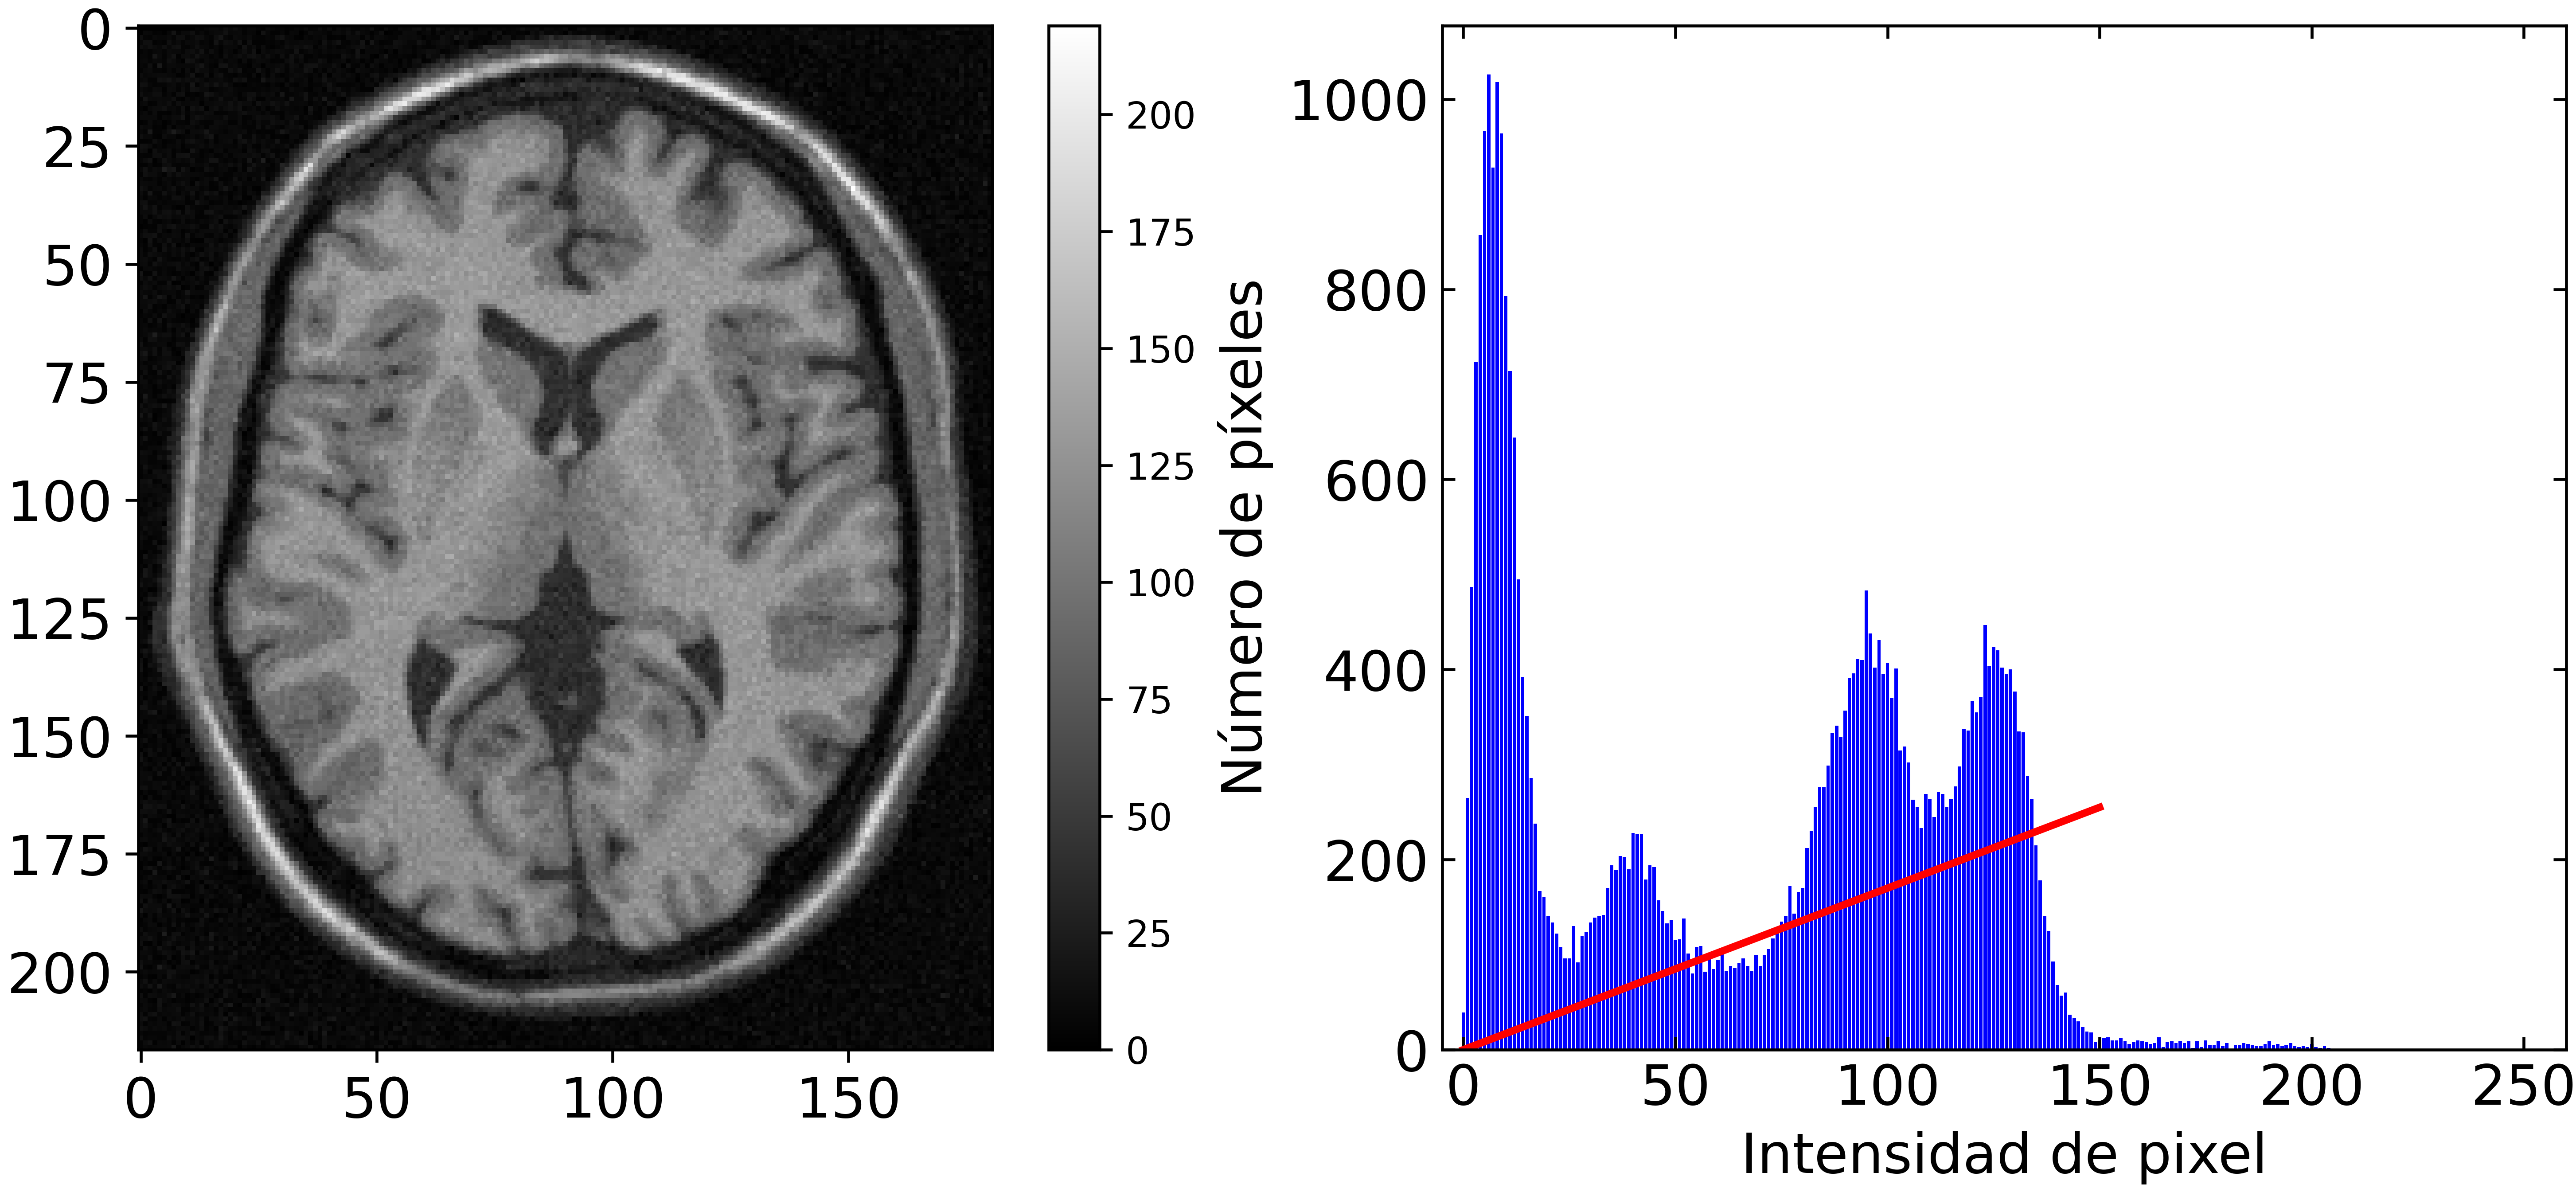
\includegraphics[width=\textwidth]{Figuras/ImageA_brute.png}
            \caption{ImagenA original junto con su histograma de intensidades.} 
            \label{fig:semilinear_a}
         \end{subfigure}
         \begin{subfigure}[h]{0.49\linewidth}
            \centering
            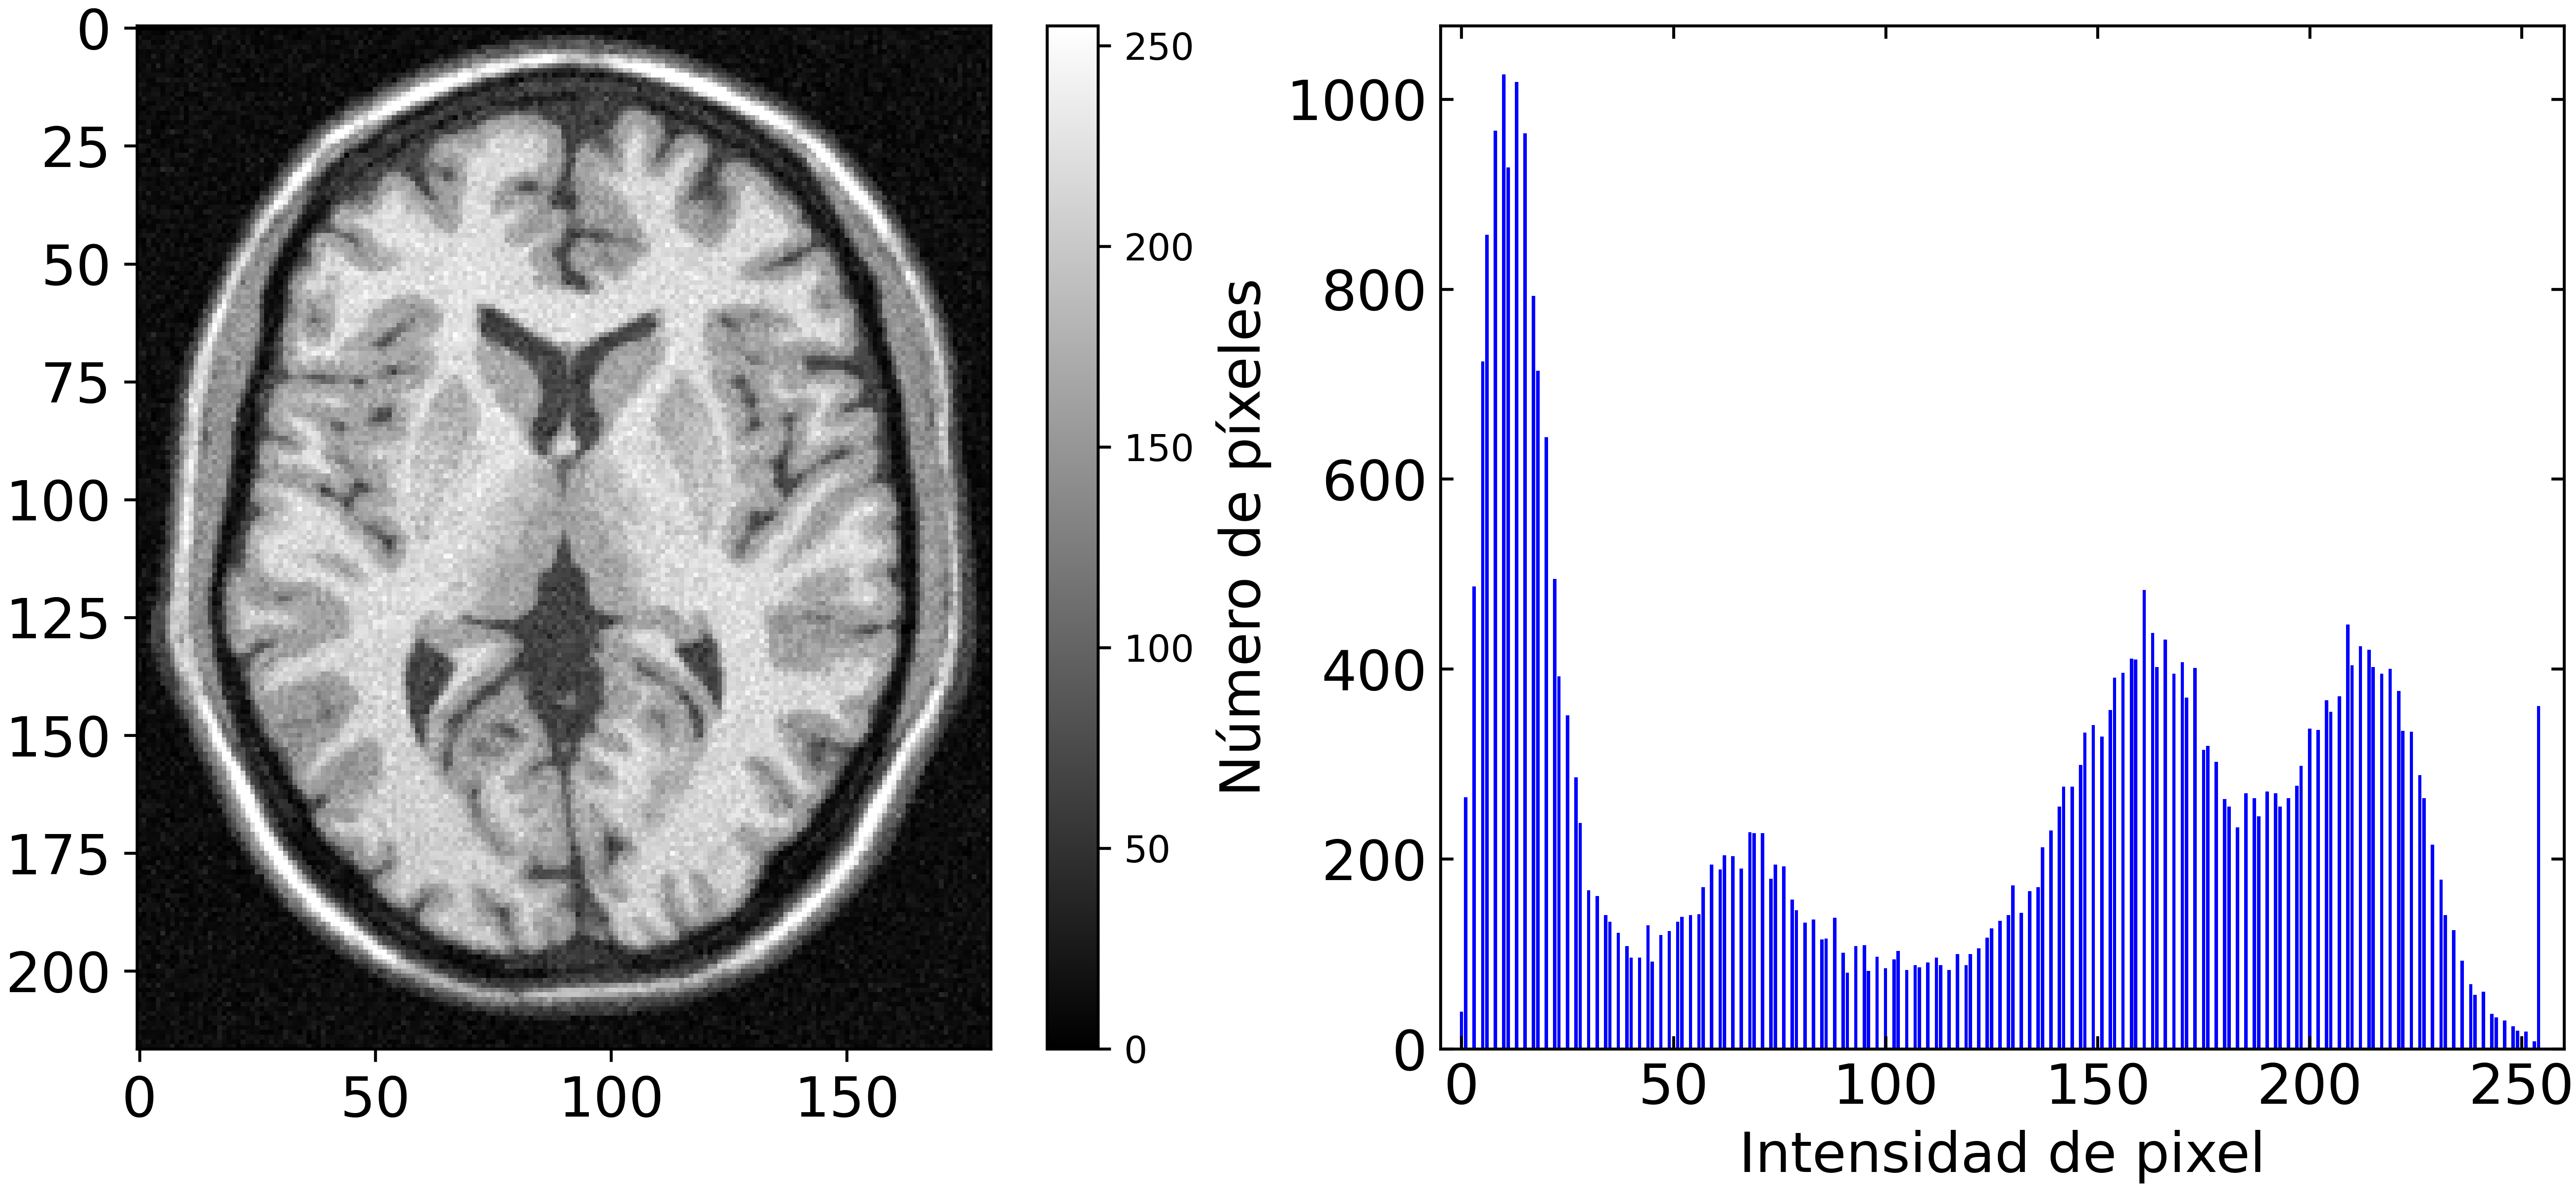
\includegraphics[width=\textwidth]{Figuras/ImageA_0_150.png}
            \caption{ImagenA transformada junto con su histograma de intensidades.}
         \end{subfigure}
    \caption{Imagen A original (a) y su transformación semilineal con $r_{min} = 0$ y $r_{min} = 150$ (b), junto con sus correspondientes histogramas de intensidades. Se observa en la imagen transformada que el histograma se corre hacia la derecha y se expande el rango dinámico.}
    \label{fig:Semilineartrans}
\end{figure}

En primer lugar, se aplicó una transformación semilinear en los niveles de gris para optimizar el rango dinámico. Este método consiste en aplicar una transformación de la forma $T(r) = a r + b$, con $r$ la intensidad del pixel, $a = (I_{max} - I_{min})/(r_{max}-r_{min})$ y $b=I_{min} - ar_{min}$, y además
\begin{itemize}
    \item Si $a r + b < I_{min} \Rightarrow T(r)=I_{min}$,
    \item Si $a r + b > I_{max} \Rightarrow T(r)=I_{max}$.
\end{itemize}
Se tomó $I_{min}=0$ e $I_{max}=255$. Para determinar los valores $r_{min}$ y $r_{max}$ de la imagen, se observa, en el histograma de la imagen original, que la mayor cantidad de valores de intensidad se concentran en el rango $[0, 150]$. Luego se toma $r_{min}=0$ y $r_{max}=150$. De esta manera, se obtiene una transformación semilinear que expande el rango dinámico de la imagen. Cabe destacar que los valores por debajo de $I_{min}$ y por encima de $I_{max}$ saturan en dichos valores, lo cual resulta en pérdida de información de la imagen original. En la Fig. \ref{fig:Semilineartrans}b se observa la transformación semilinear junto con su correspondiente histograma de intensidades. Se observa que el histograma se corre hacia la derecha y se expande el rango dinámico. Además, en el histograma de la imagen transformada que se acumulan pixeles con intensidad máxima $I_{max}$.

En el histograma de la imagen original se distinguen 4 picos de intensidad, que corresponden 4 regiones de la imagen; De menor a mayor valor de intensidad: Fondo, líquido, materia gris y materia blanca. Se eligieron convenientemente los valores de $r_{min}$ y $r_{max}$ para que la transformación semilinear resalte cada una de estas regiones. El resultado se muestra en la Fig. \ref{fig:Semilineartrans_region}.

\begin{figure}[H]
    \centering
         \begin{subfigure}[h]{0.24\linewidth}
            \centering
            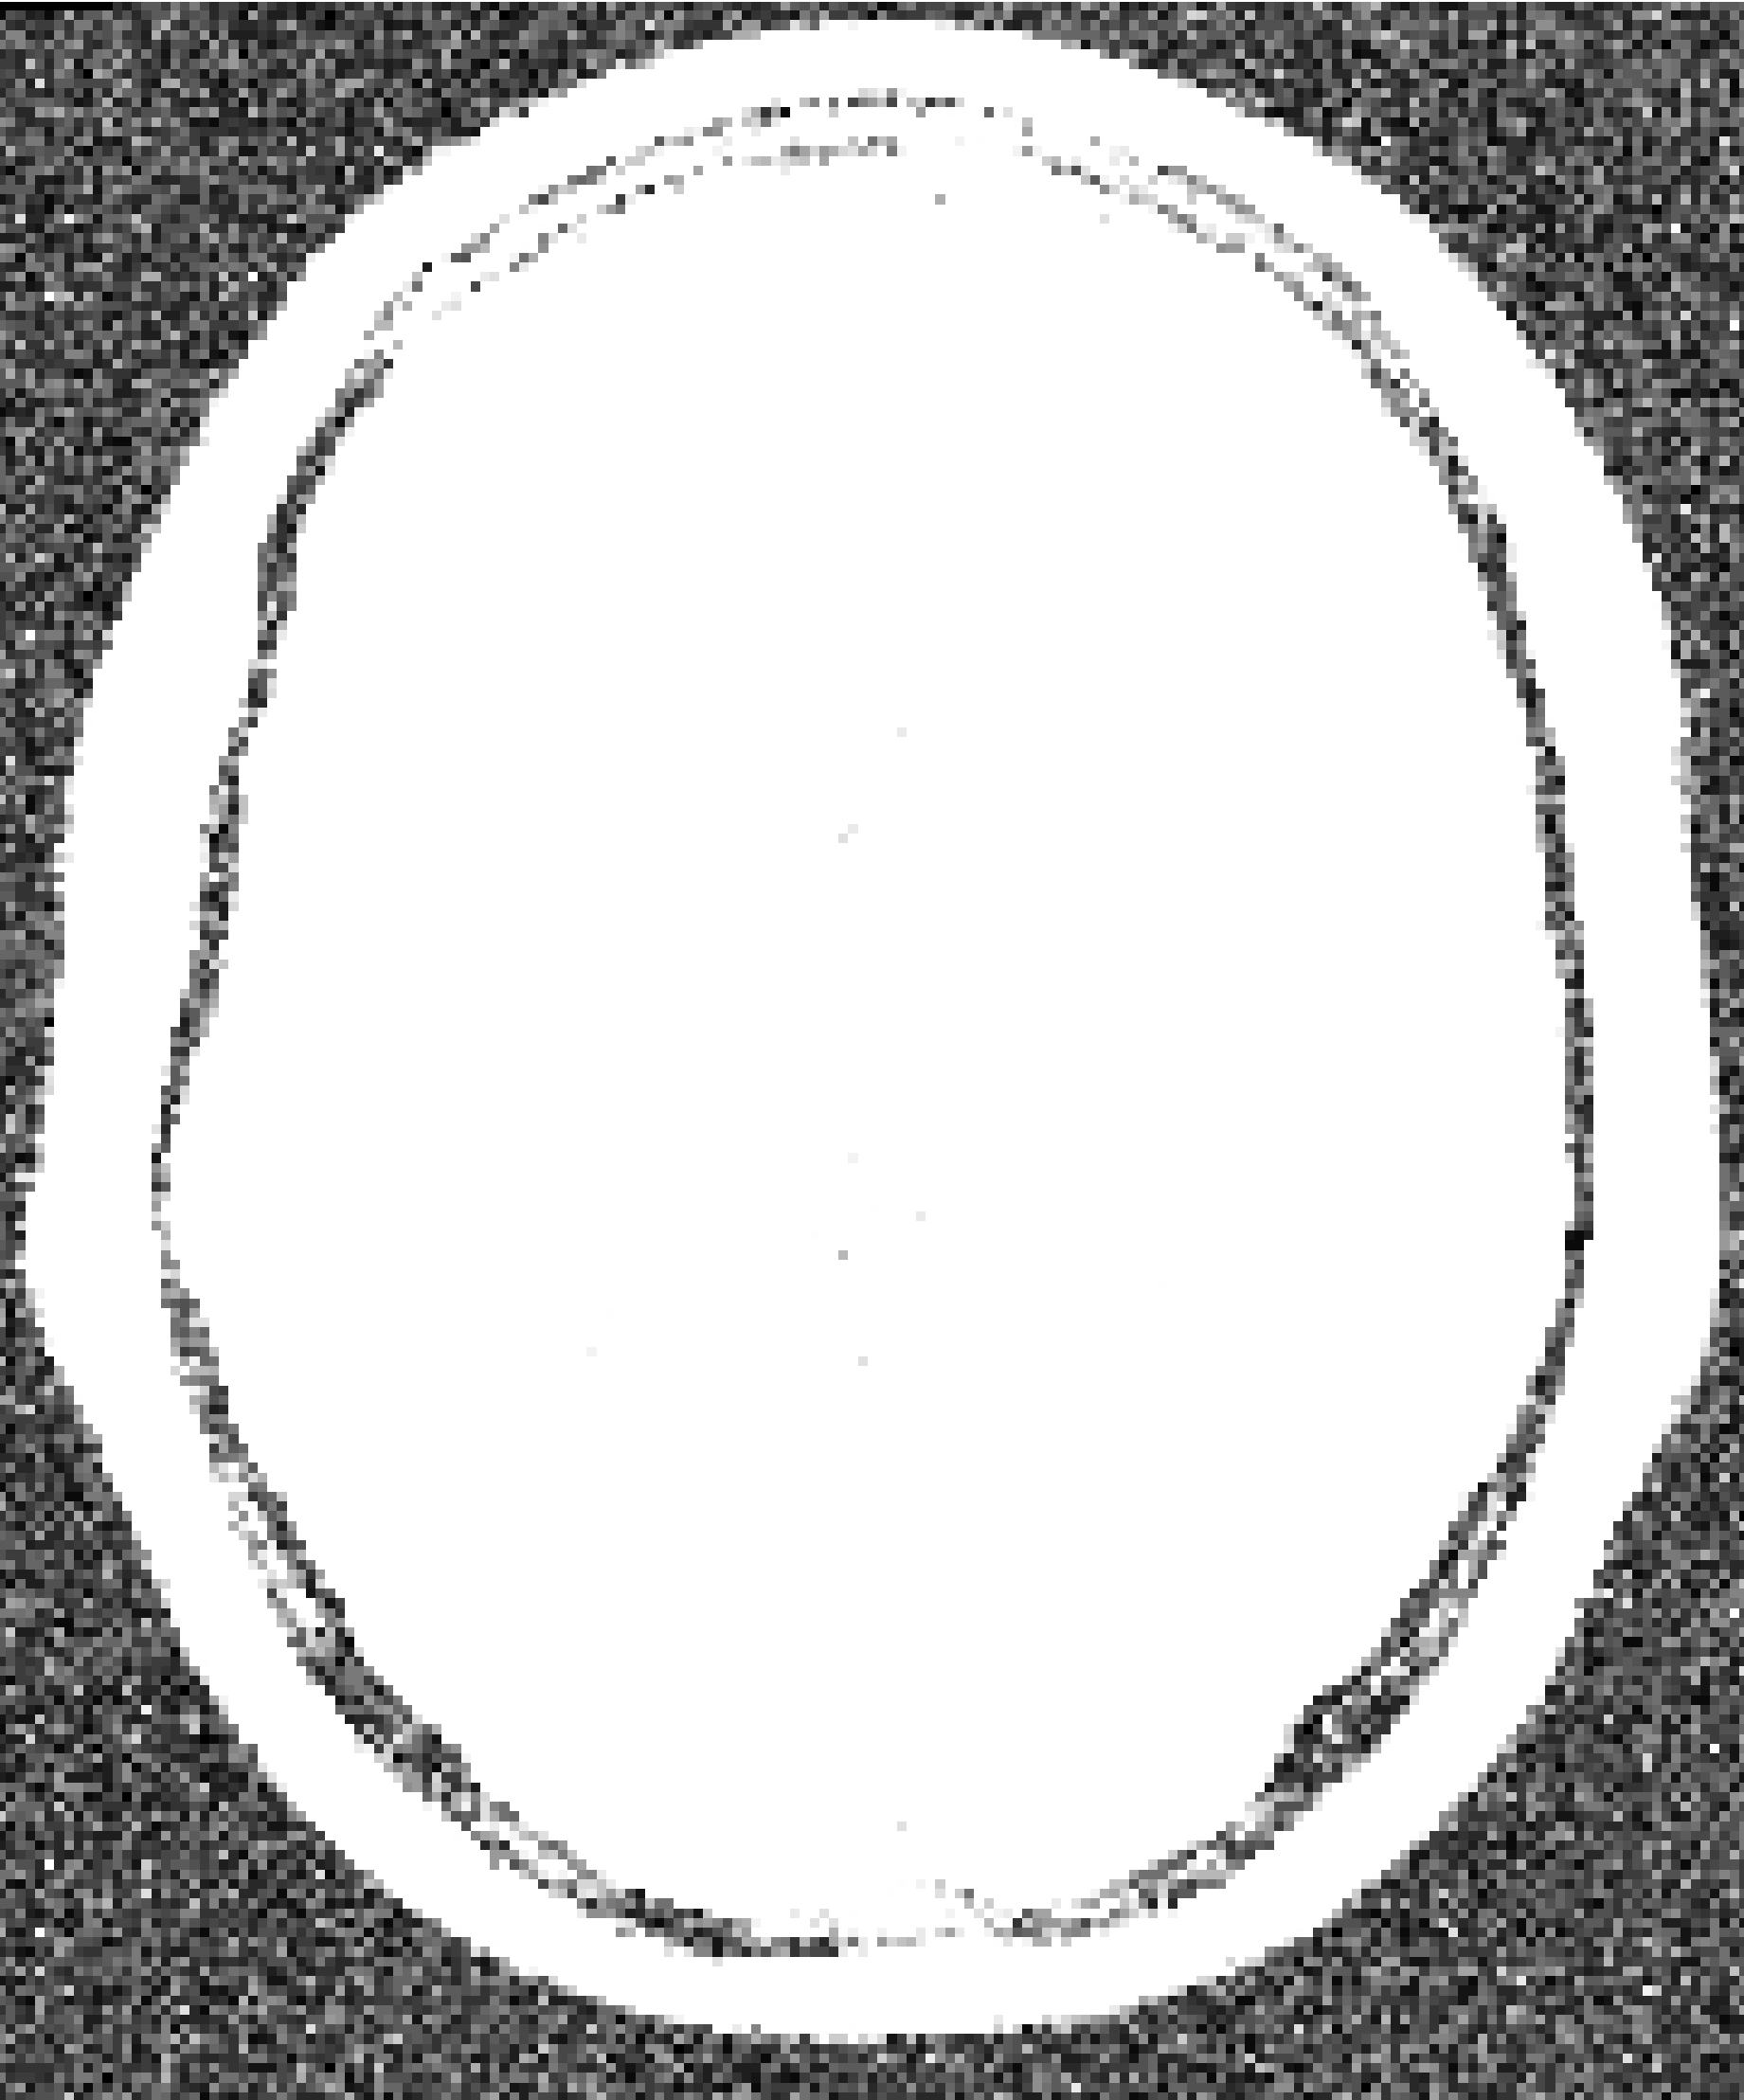
\includegraphics[width=\textwidth]{Figuras/ImageA_0_25.png}
            \caption{Fondo} 
         \end{subfigure}
         \begin{subfigure}[h]{0.24\linewidth}
            \centering
            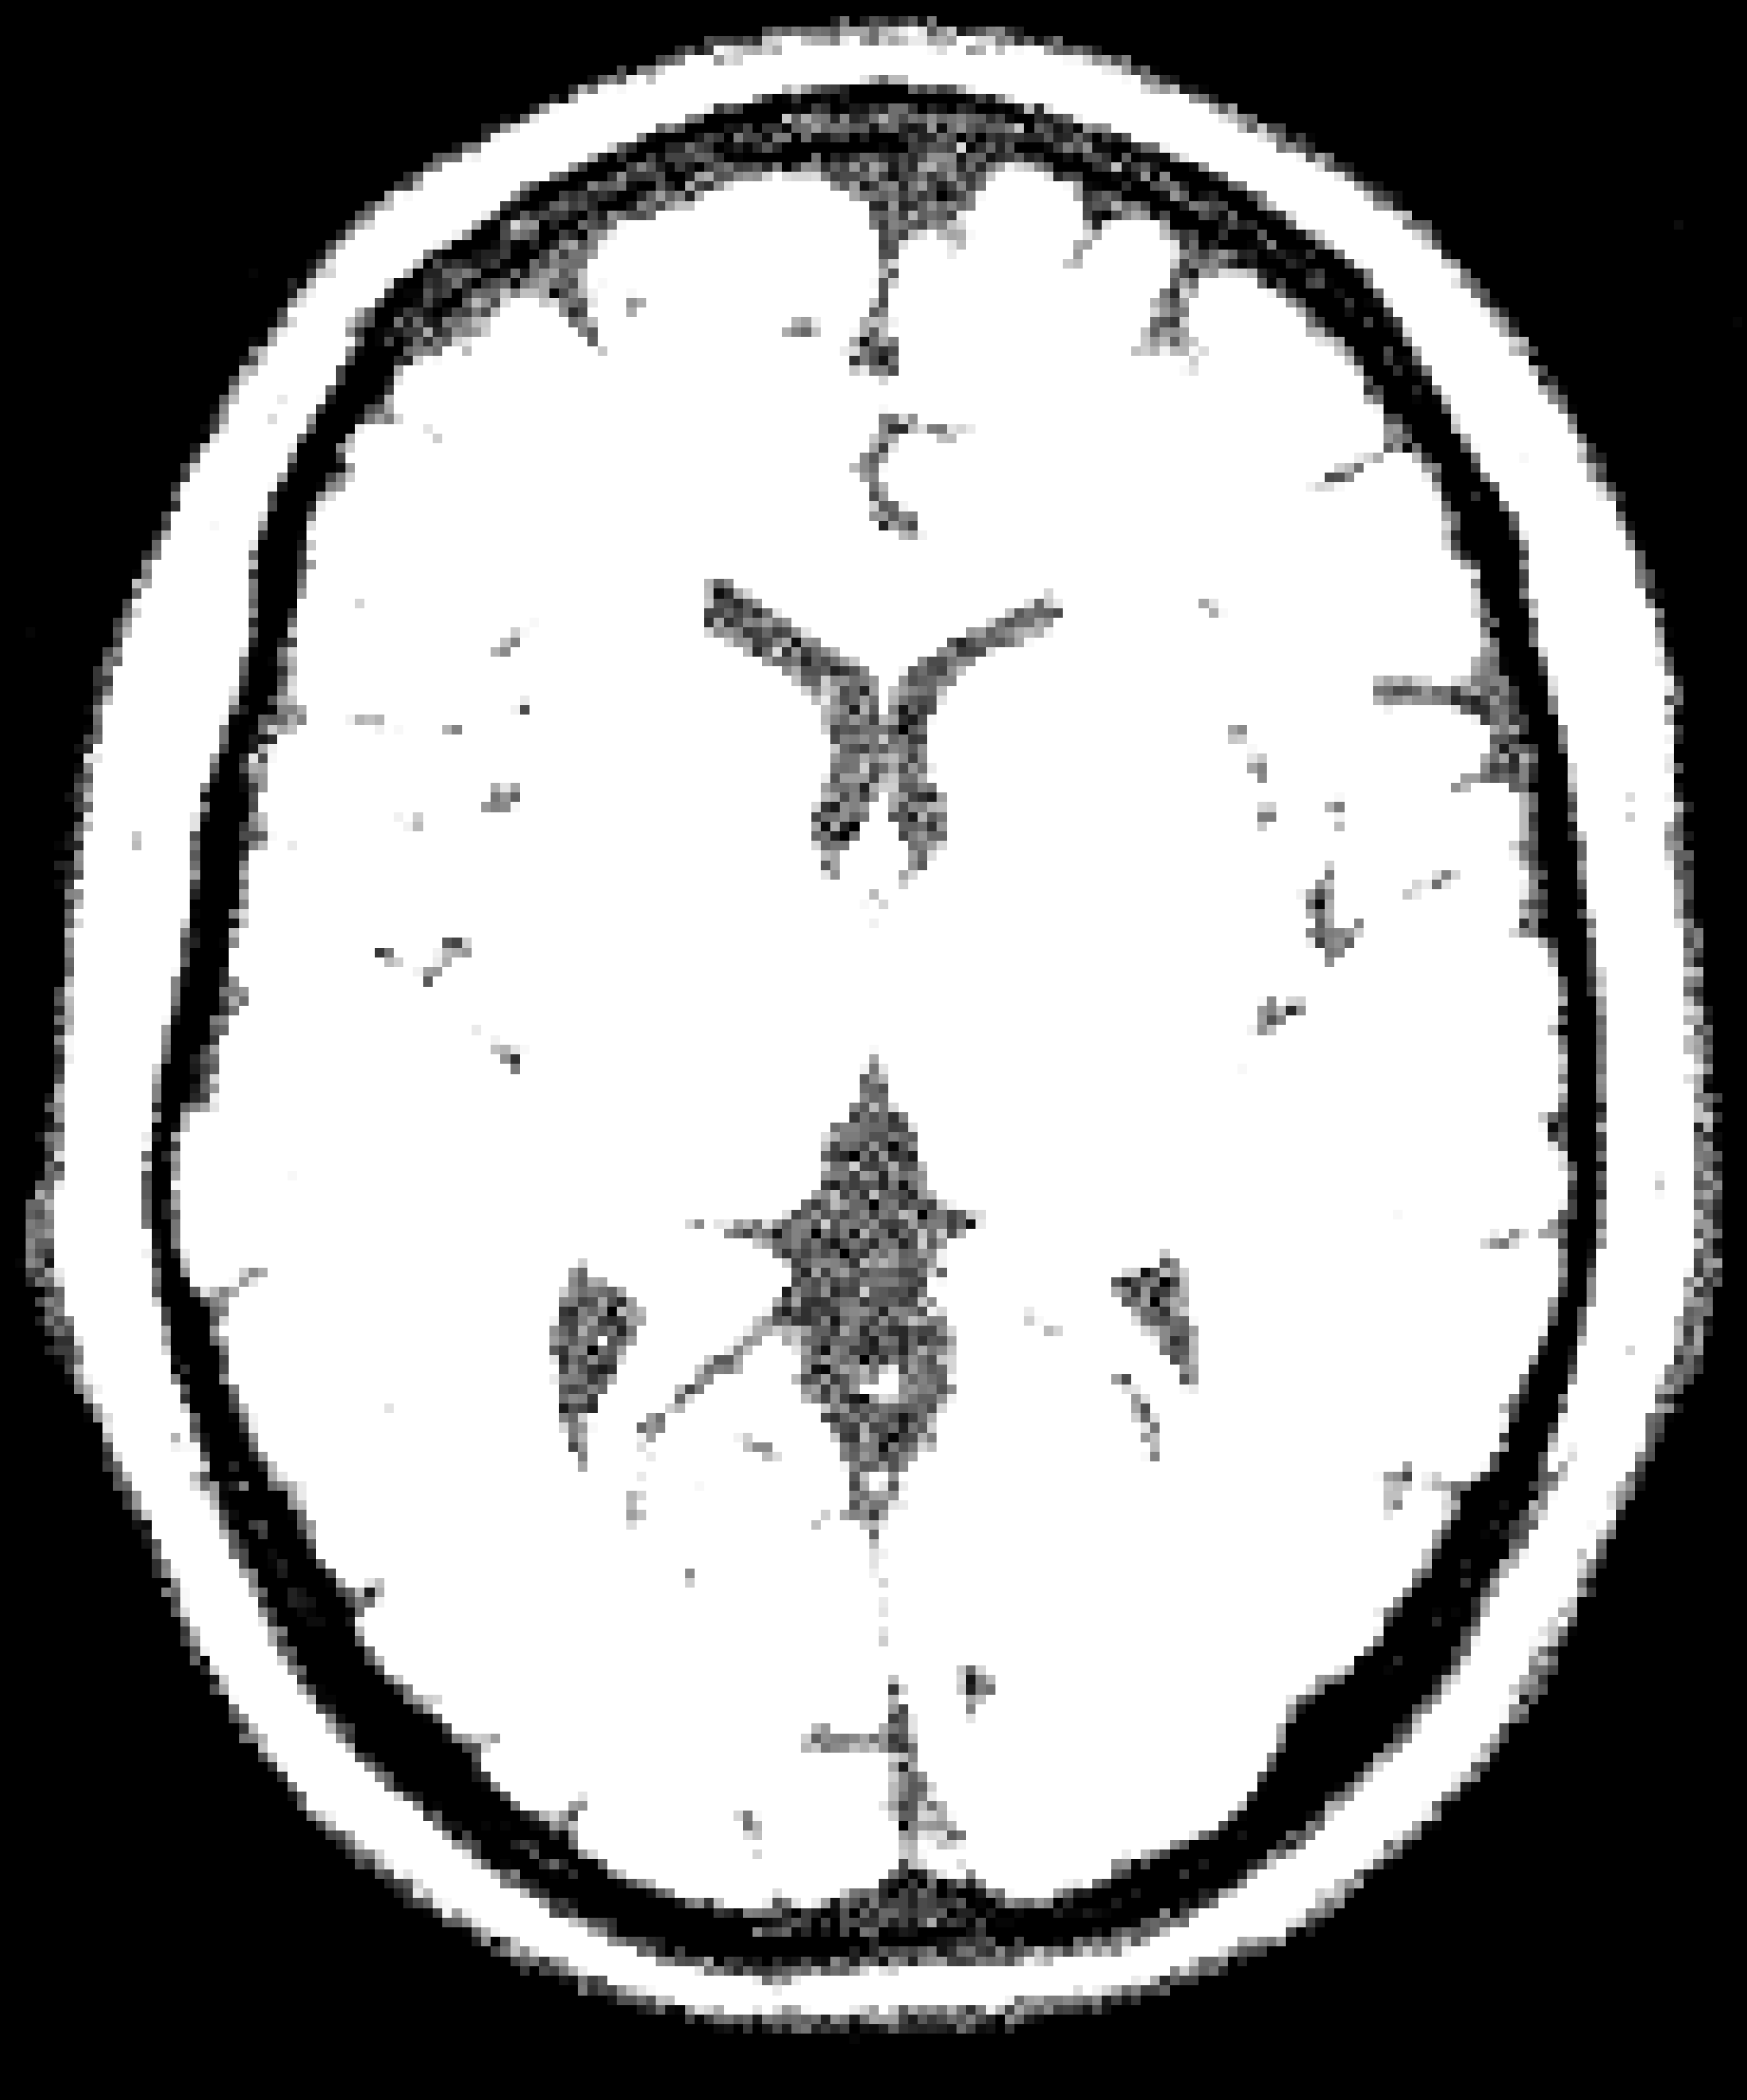
\includegraphics[width=\textwidth]{Figuras/ImageA_25_62.png}
            \caption{Líquido} 
         \end{subfigure}
         \begin{subfigure}[h]{0.24\linewidth}
            \centering
            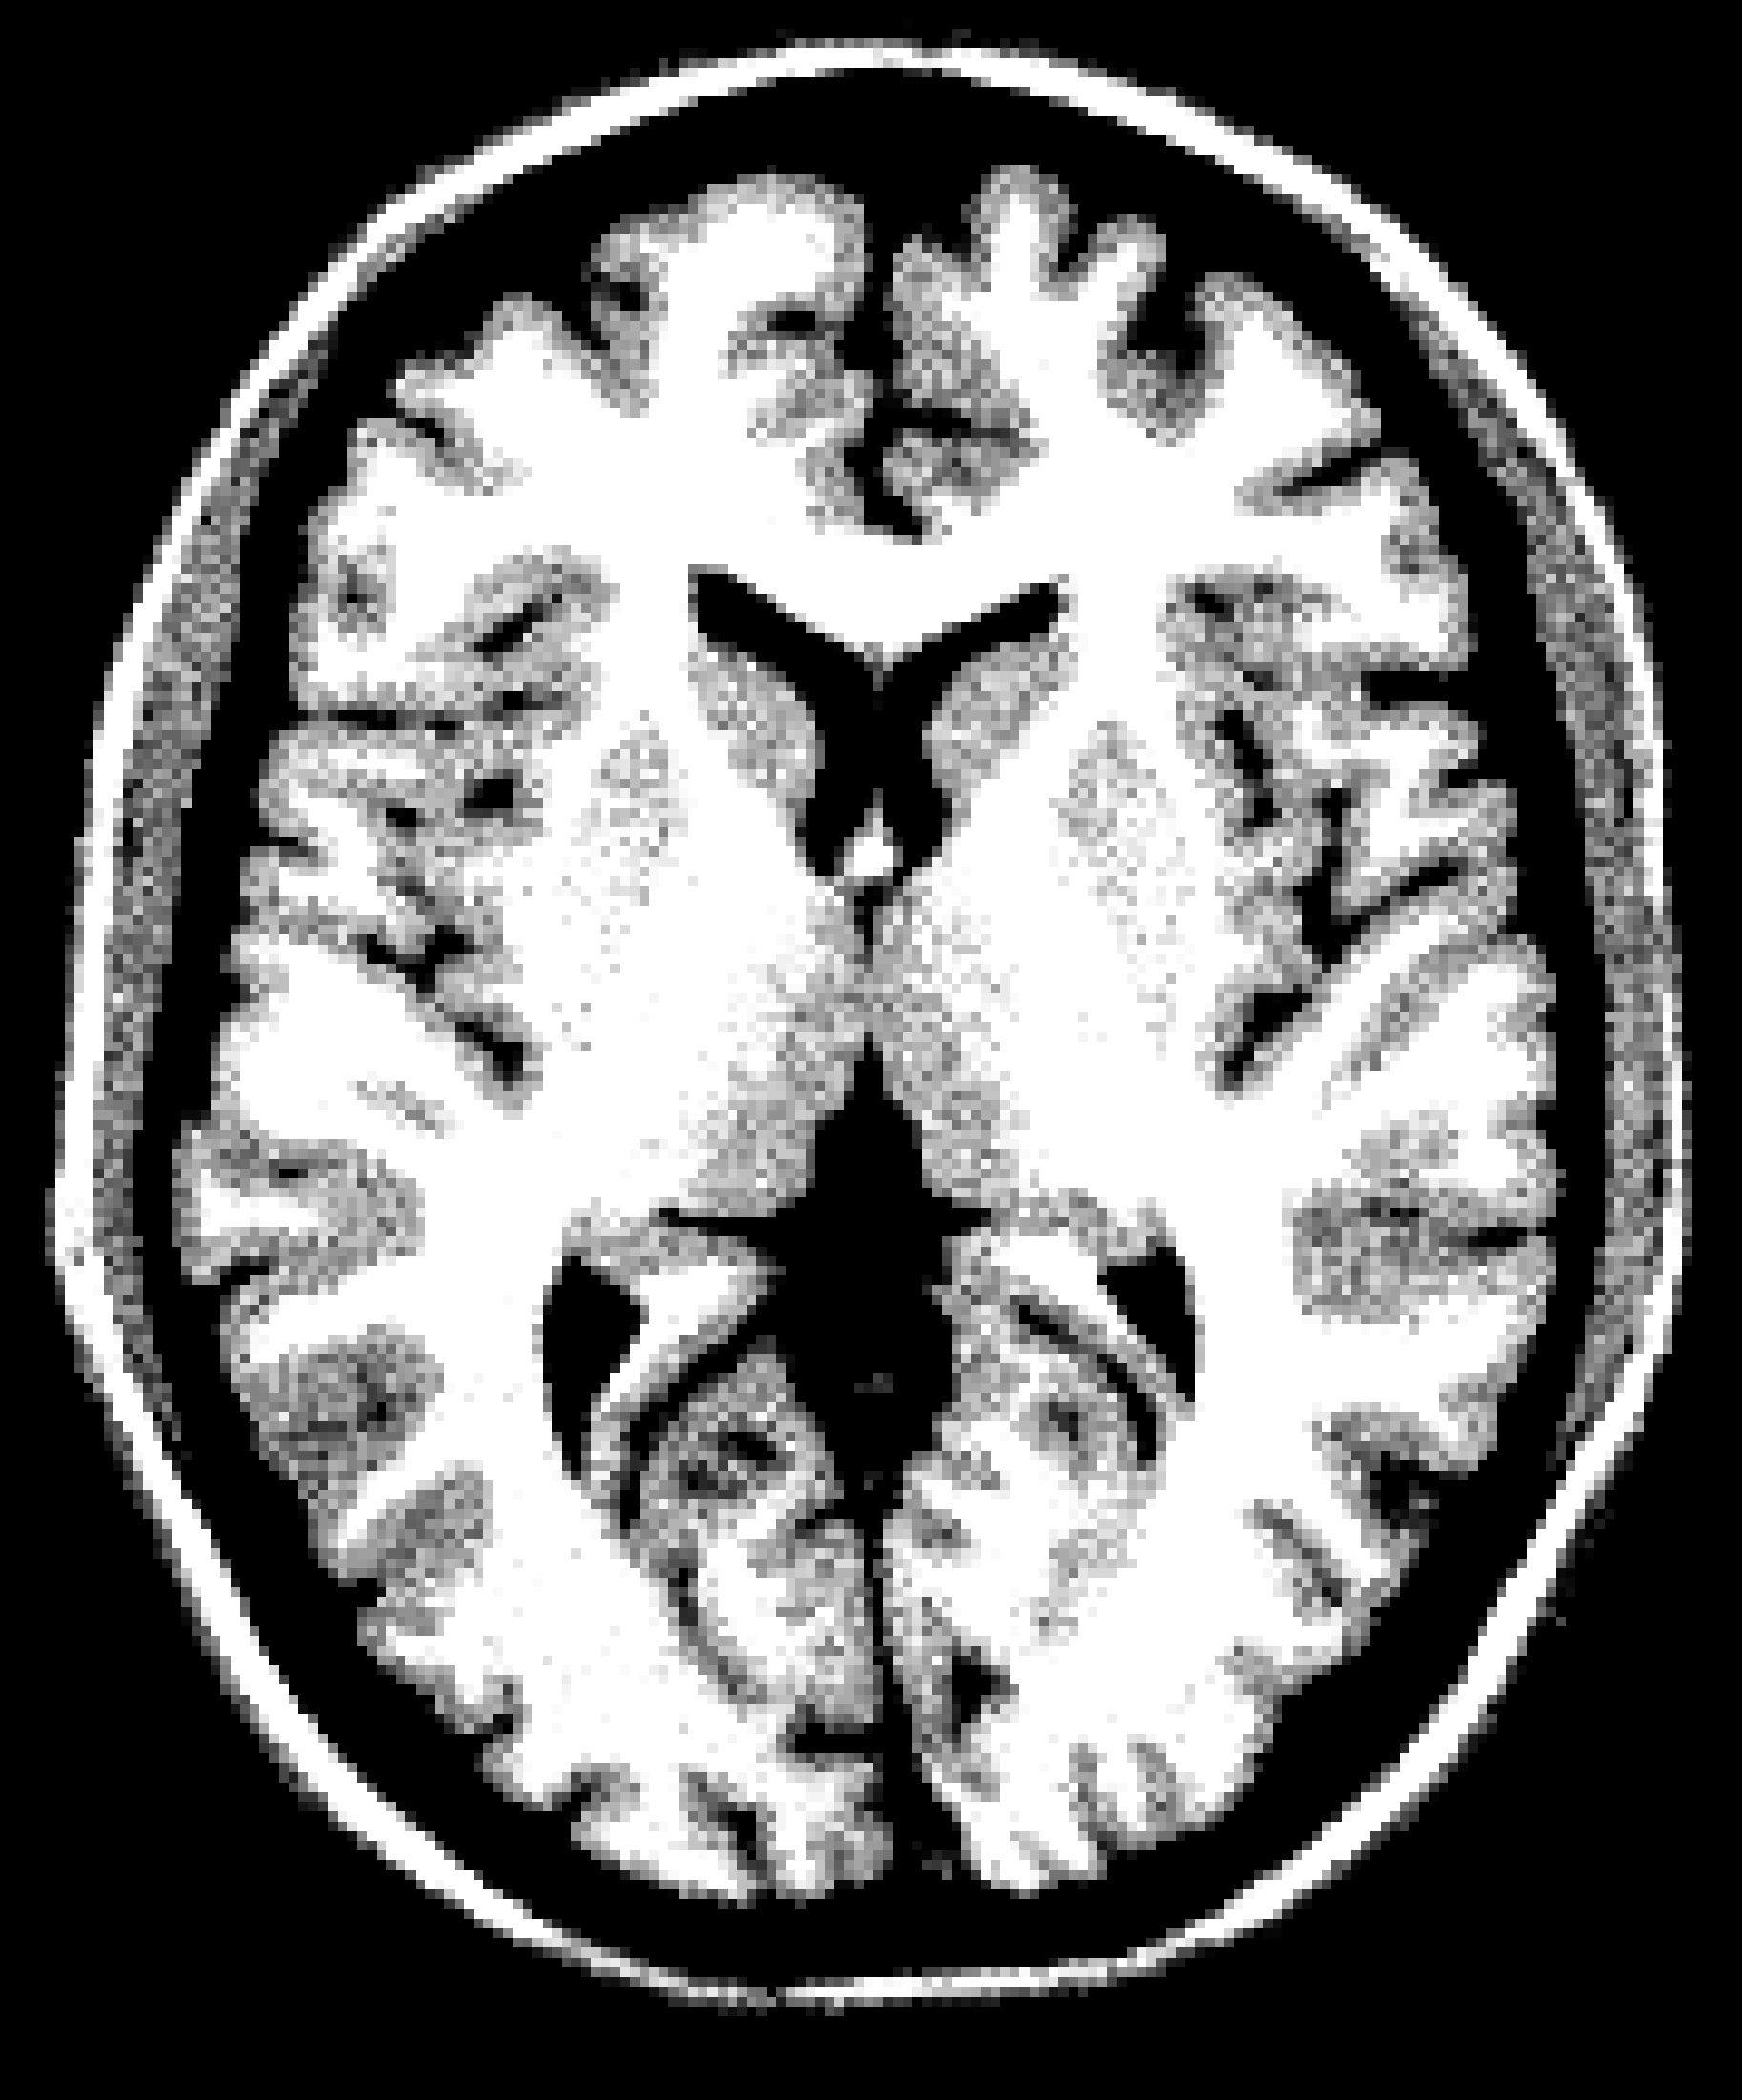
\includegraphics[width=\textwidth]{Figuras/ImageA_62_113.png}
            \caption{Materia gris} 
         \end{subfigure}
         \begin{subfigure}[h]{0.24\linewidth}
            \centering
            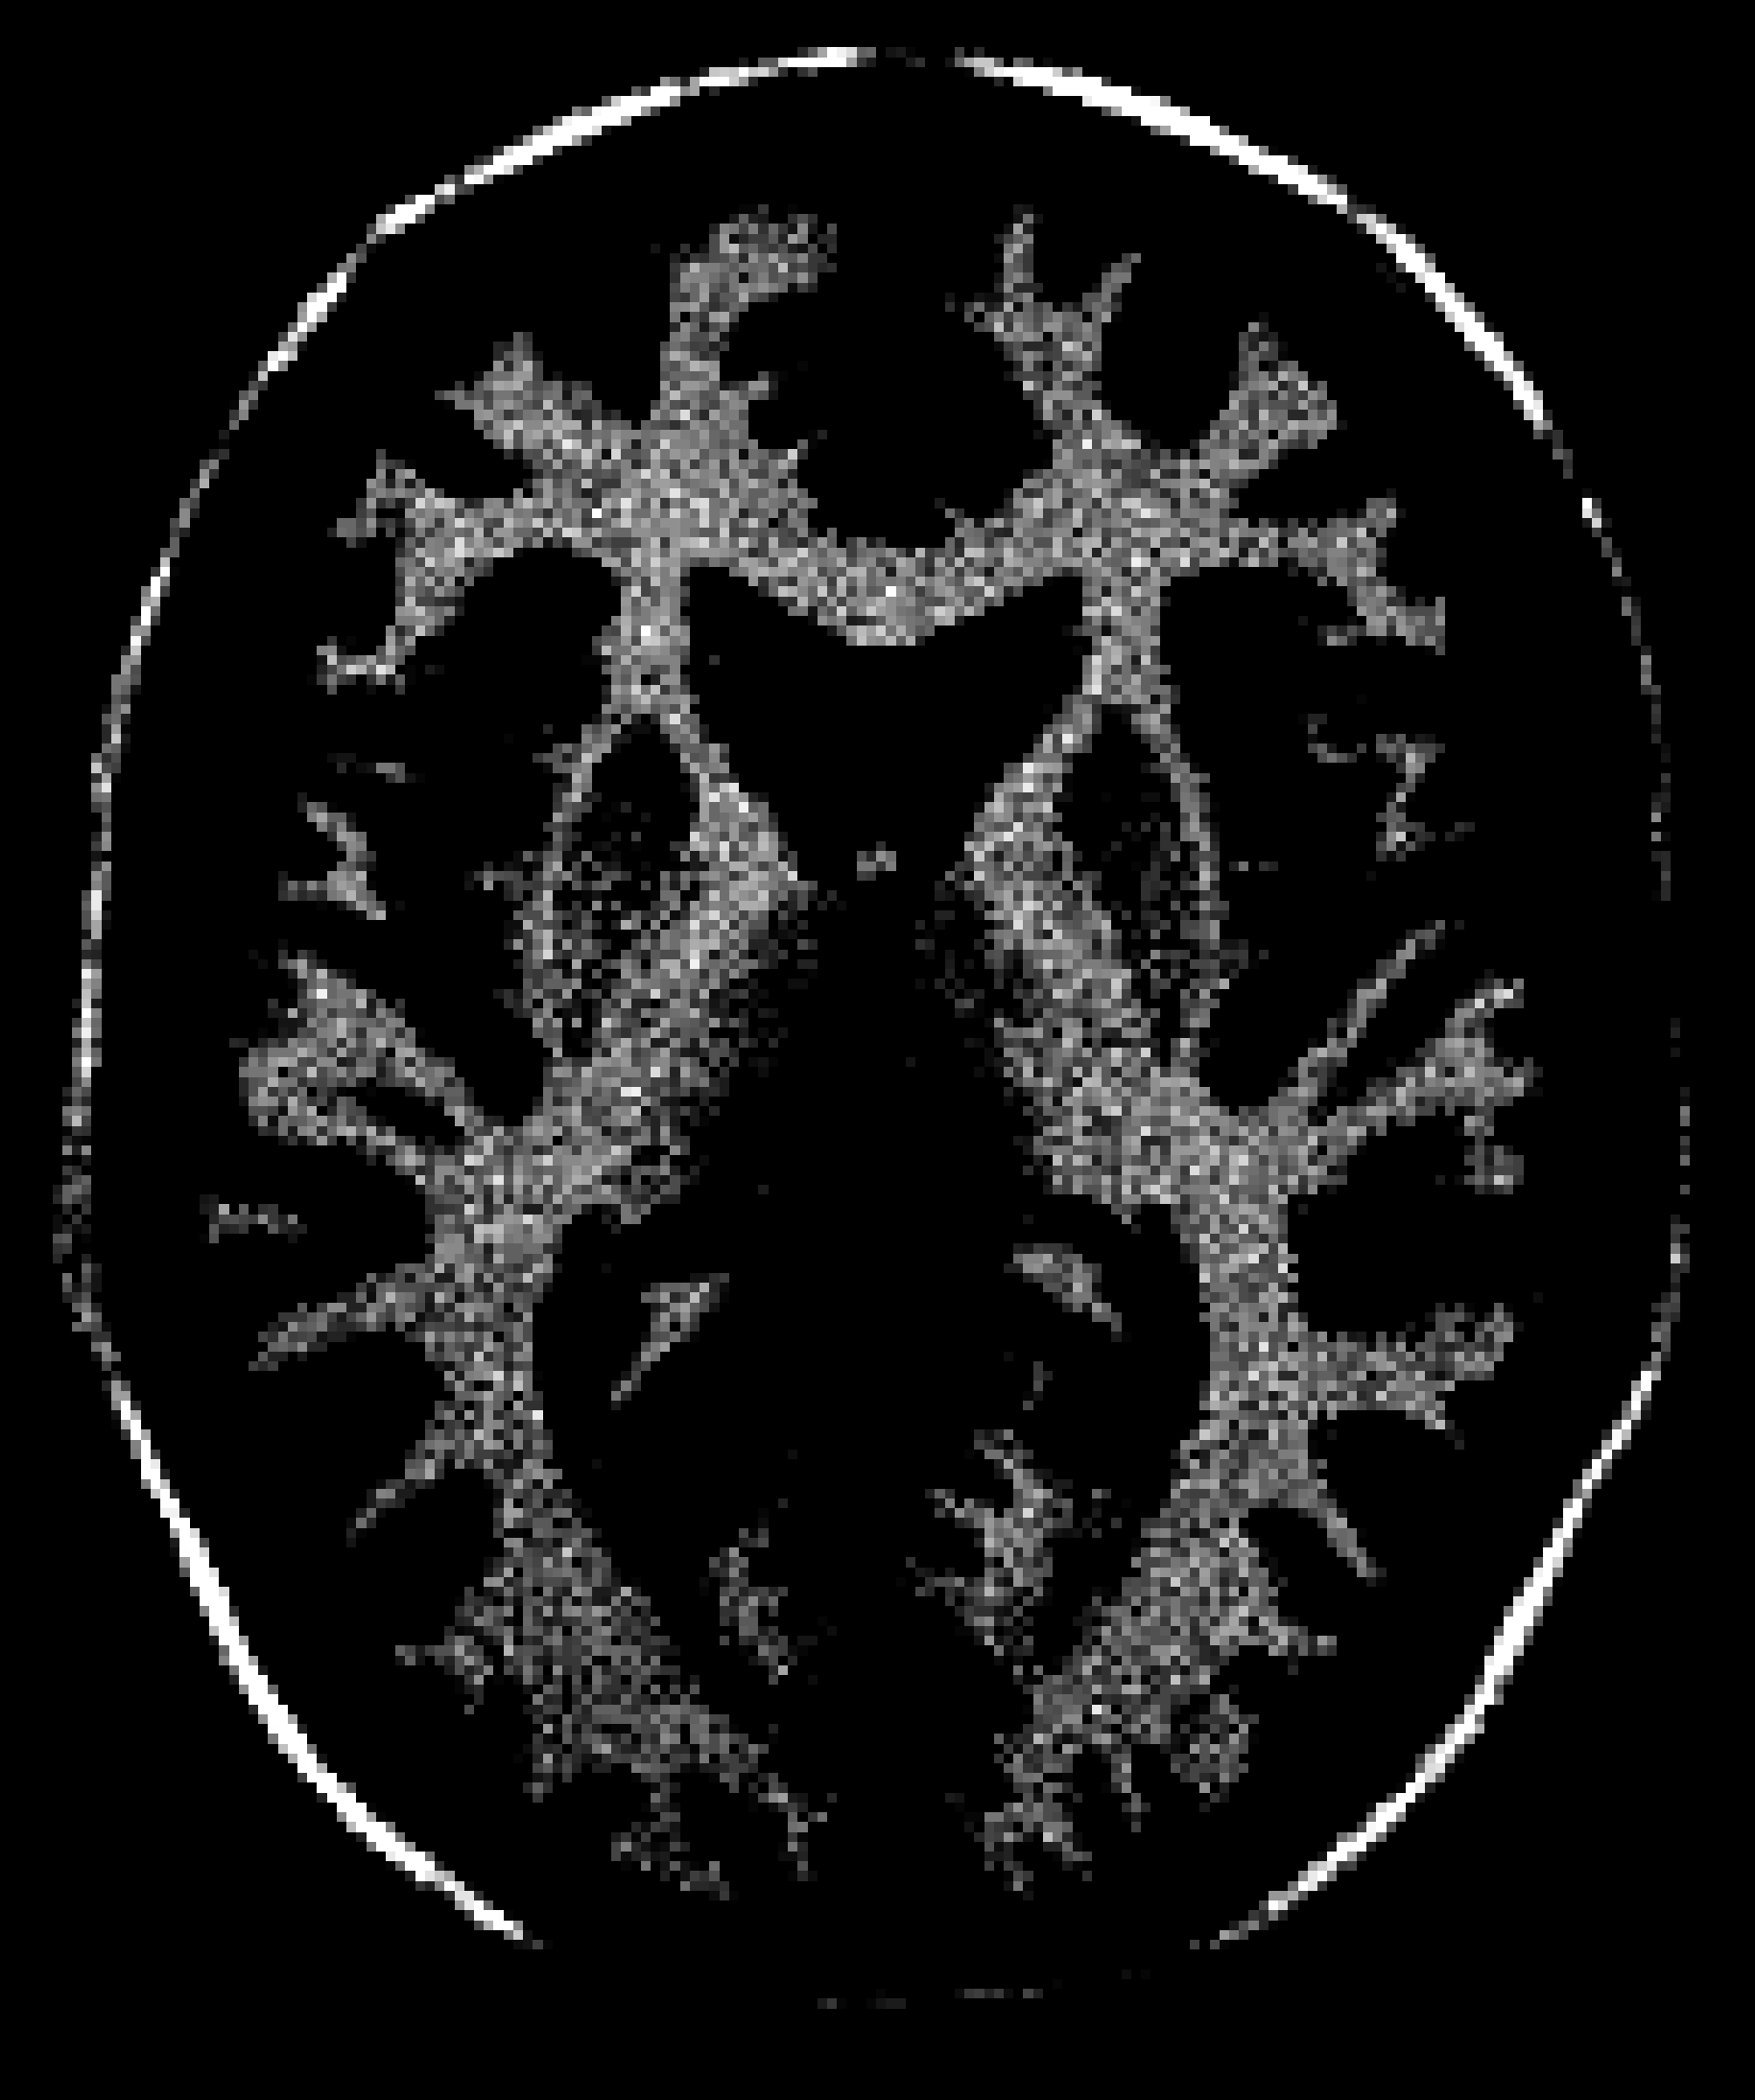
\includegraphics[width=\textwidth]{Figuras/ImageA_113_150.png}
            \caption{Materia blanca} 
         \end{subfigure}
    \caption{Transformación semilinear aplicada a distintas regiones de la imagen original.%(a) Fondo (b) Líquido (c) Materia gris (d) Materia blanca.
    }
    \label{fig:Semilineartrans_region}
\end{figure}

\subsection{Ecualización}

Por otro lado, se ecualizó la $\verb|ImagenA.pgm|$ como se muestra en la Fig. \ref{fig:EQ}. 

\begin{figure}[H]
    \centering
        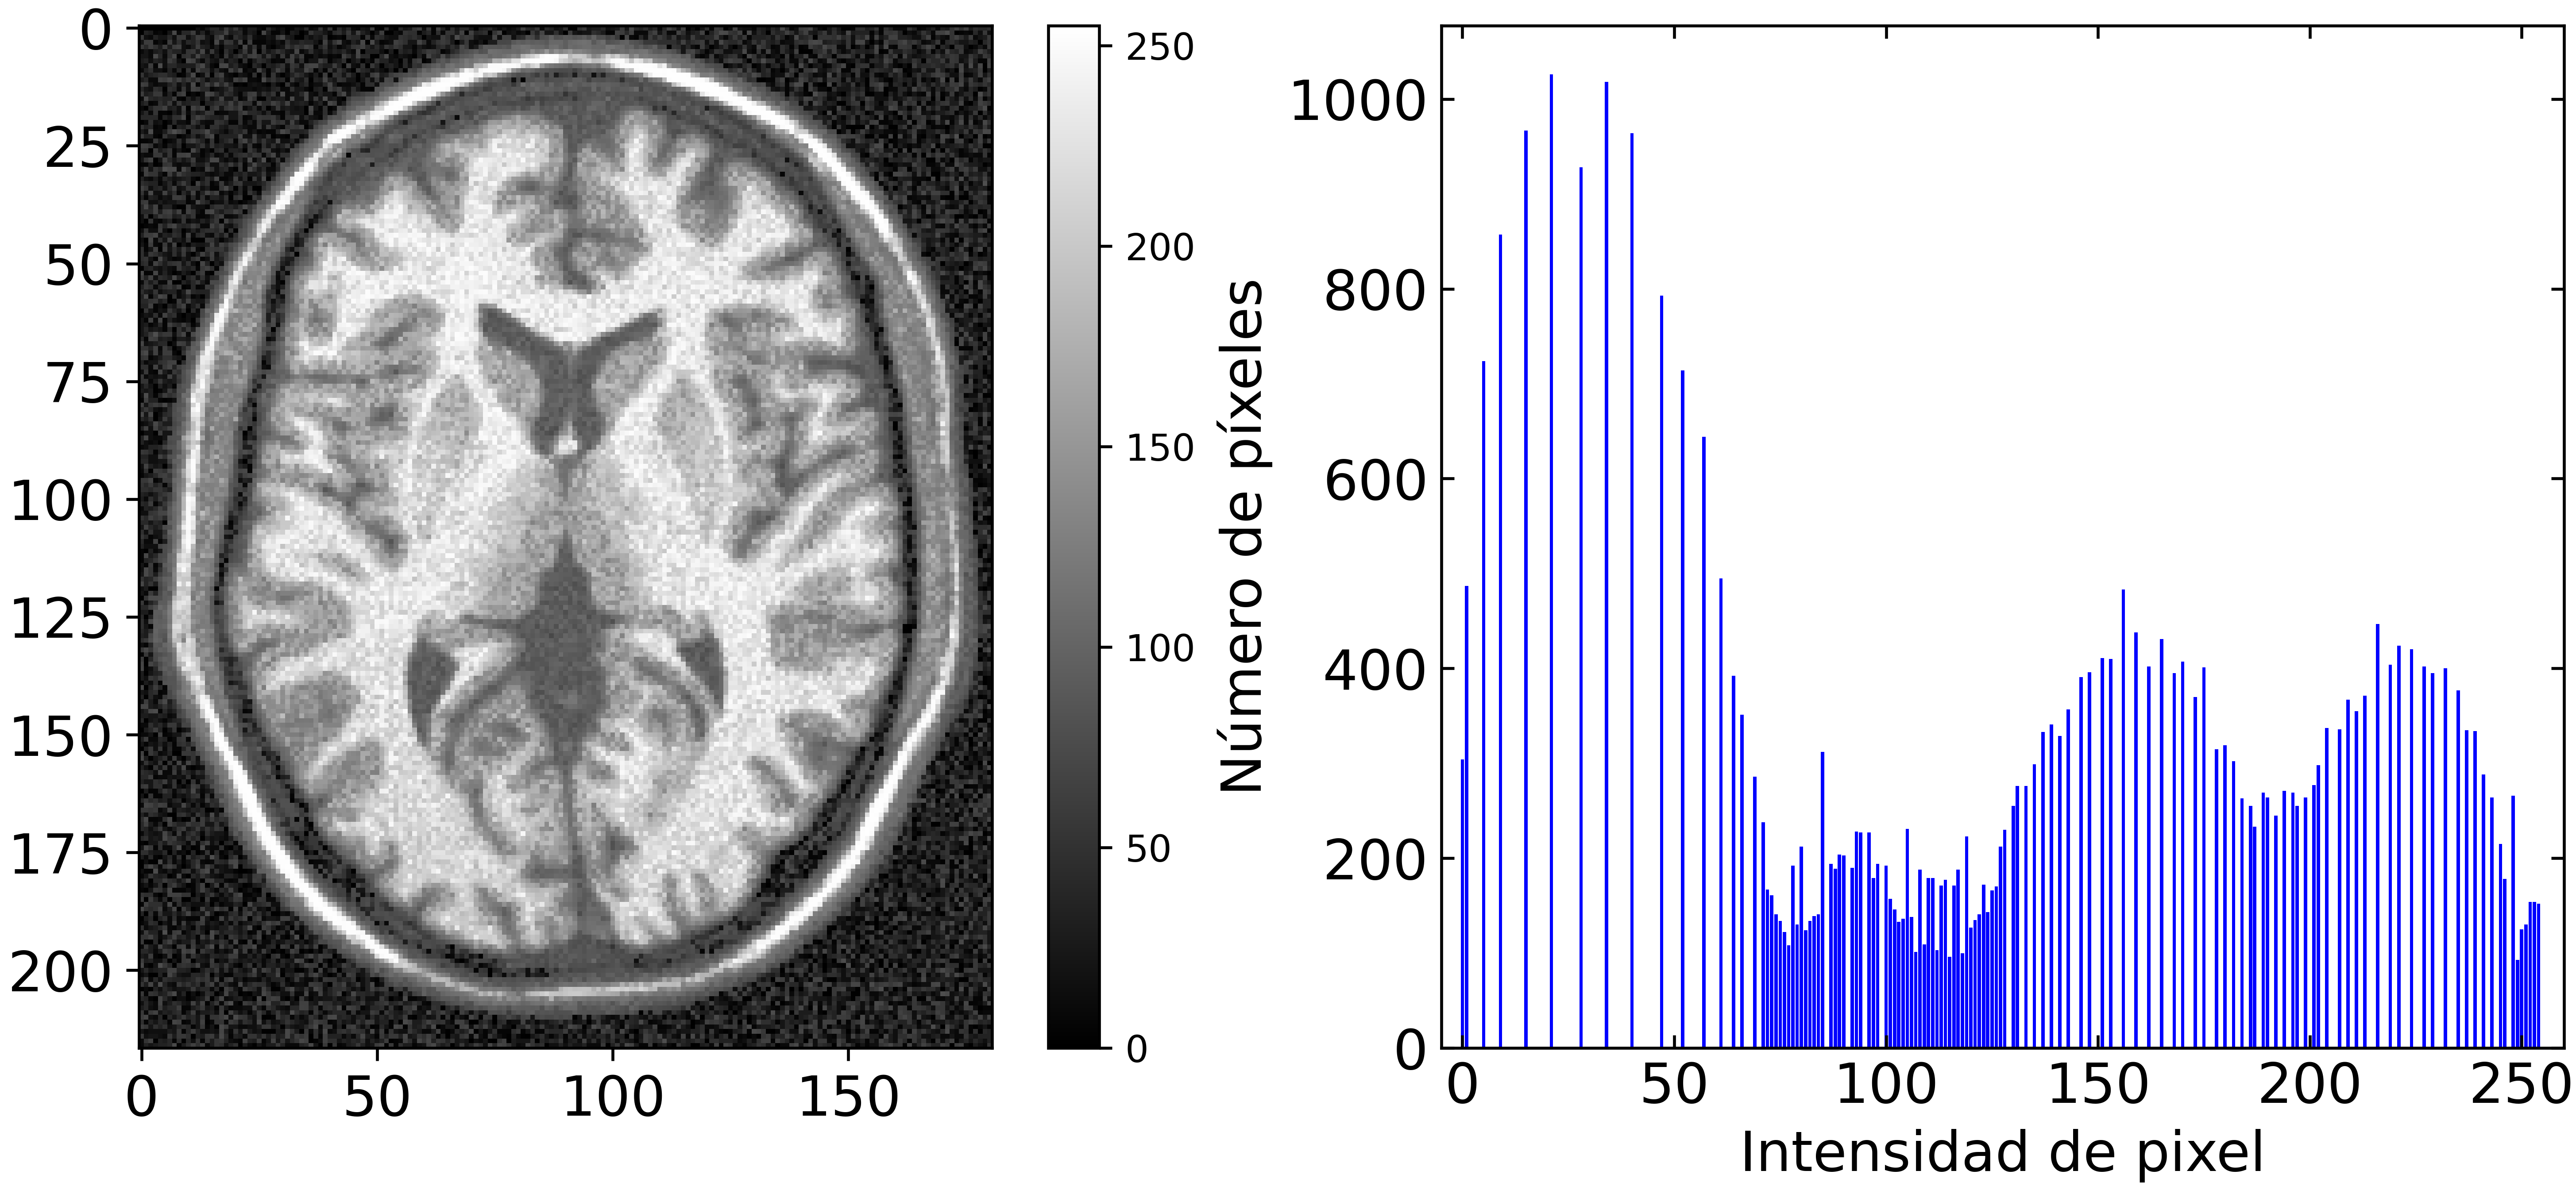
\includegraphics[width=0.75\textwidth]{Figuras/ImageA_EQ_hist.png}
    \caption{ImagenA ecualizada junto con su histograma de intensidades.} 
    \label{fig:EQ}
\end{figure}

La ecualización corresponde a una trasnformación de la forma
\begin{equation}
    T(r_k) = (r_{max} - r_{min}) \sum_{i=0}^{k} P_r(r_i)
\end{equation}
donde $P_r(r_i)$ es la distribución de probabilidad de que un pixel tenga intensidad $i$. En particular, se toma esta distribución normalizando el histograma de intensidades de la imagen original (Fig. \ref{fig:semilinear_a}). Se observa que se expande el rango dinámico, mejorando el contraste de la imagen sin acumulación de intensidades como sucedía en la transformación semilinear.

\subsection{Transformación binaria y transformación gamma}

Se pueden realizar otras transformaciones de contraste, como la binarización de la imagen, que consiste en transformar la imagen según 
\begin{equation}
    T(r) = 
    \begin{cases}
    0 & \text{si } r \geq 128 \\
    255 & \text{si } r < 128
    \end{cases}
\end{equation}
o una transformación según una ley de potencias de la forma
\begin{equation}
    T(r) = I_{max} \biggr( \frac{r}{r_{max}}\biggr)^\gamma
\end{equation}
donde se tomó $I_{max} = 255$ y distintos valores de $\gamma$.

En la Fig. \ref{fig:binarytrans} se muestra la imagen binarizada de la imagen A original. Esta transformación muestra en negro los valores de la imagen por encima de un cierto umbral, en este caso 128, y en blanco el resto. Se utilizó 255 en lugar de 1 para mejorar el contraste de la imagen. Esto sirve para resaltar estructuras por encima de dicho umbral eliminando el resto de información de la imagen.

\begin{figure}[H]
   \centering
       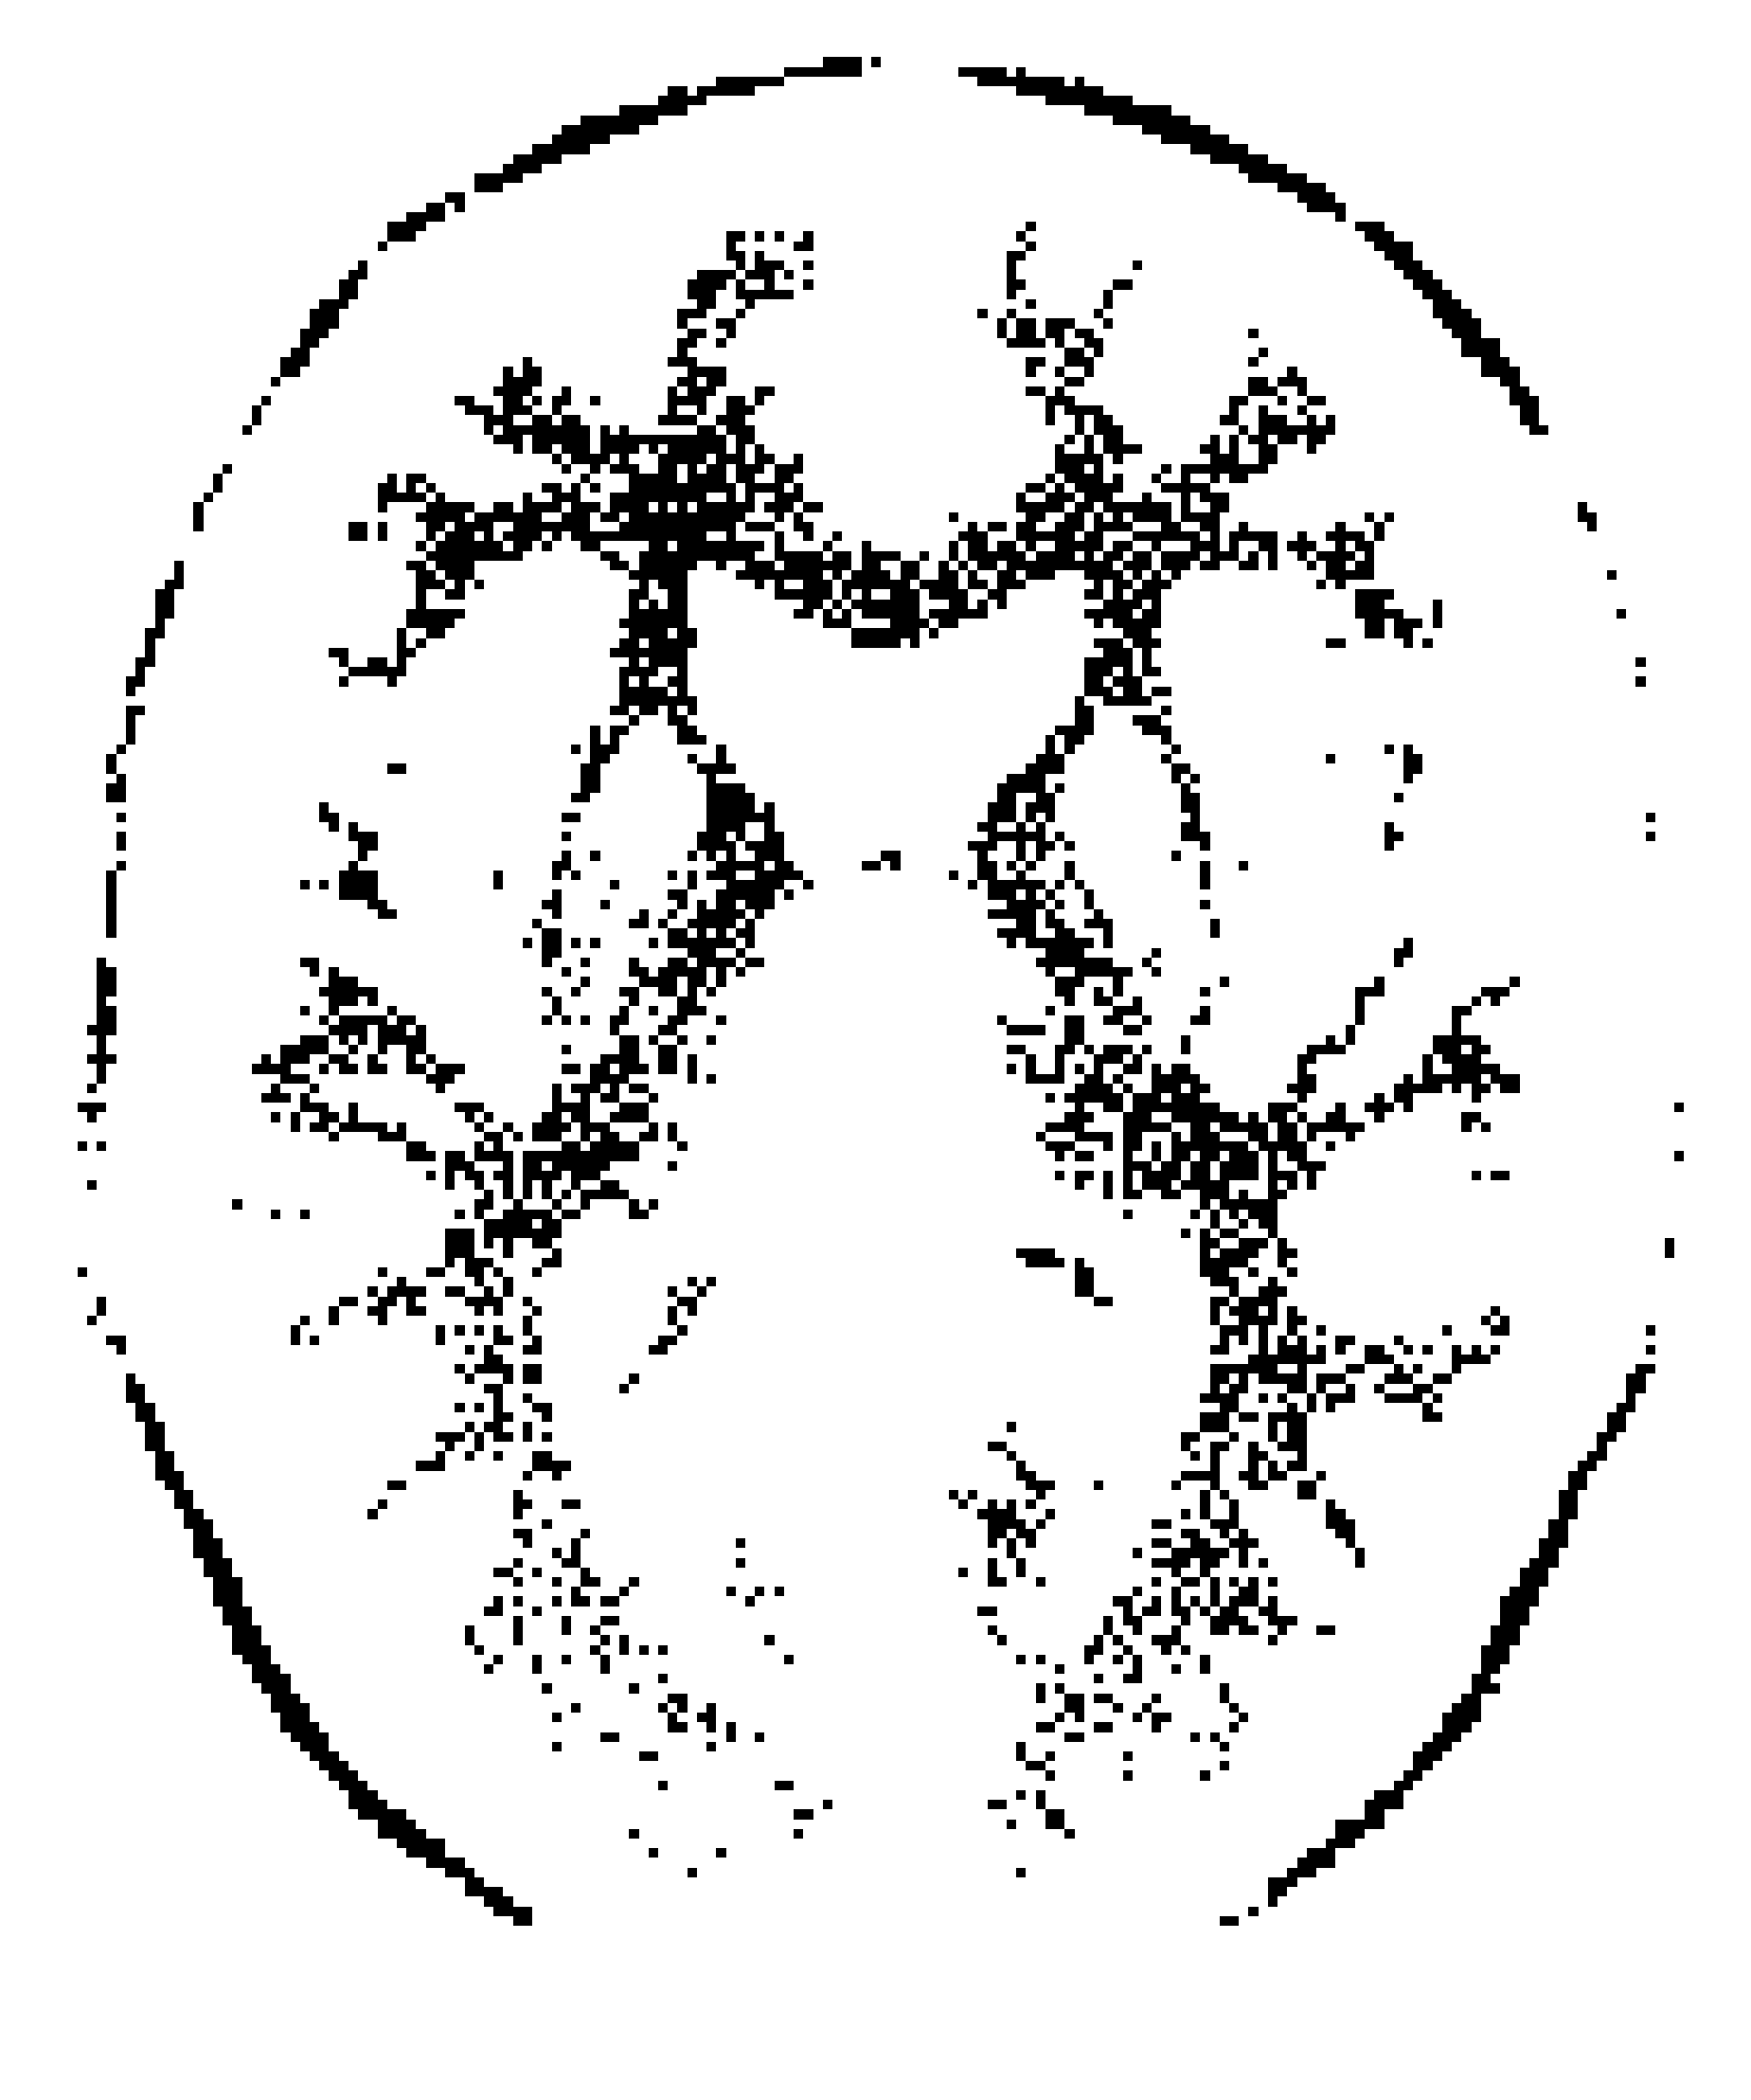
\includegraphics[width=0.25\textwidth]{Figuras/ImageA_binary.png}
   \caption{Transformación binaria aplicada a la imagenA original.}
   \label{fig:binarytrans}
\end{figure}

En la Fig. \ref{fig:Exptrans} se muestra la transformación $\gamma$ aplicada a la imagen A original. En este caso, se ve que valores de $\gamma < 1$ generan una imagen más brillante y valores de $\gamma > 1 $ más oscura.

\begin{figure}[H]
    \centering
         \begin{subfigure}[h]{0.2\textwidth}
            \centering
            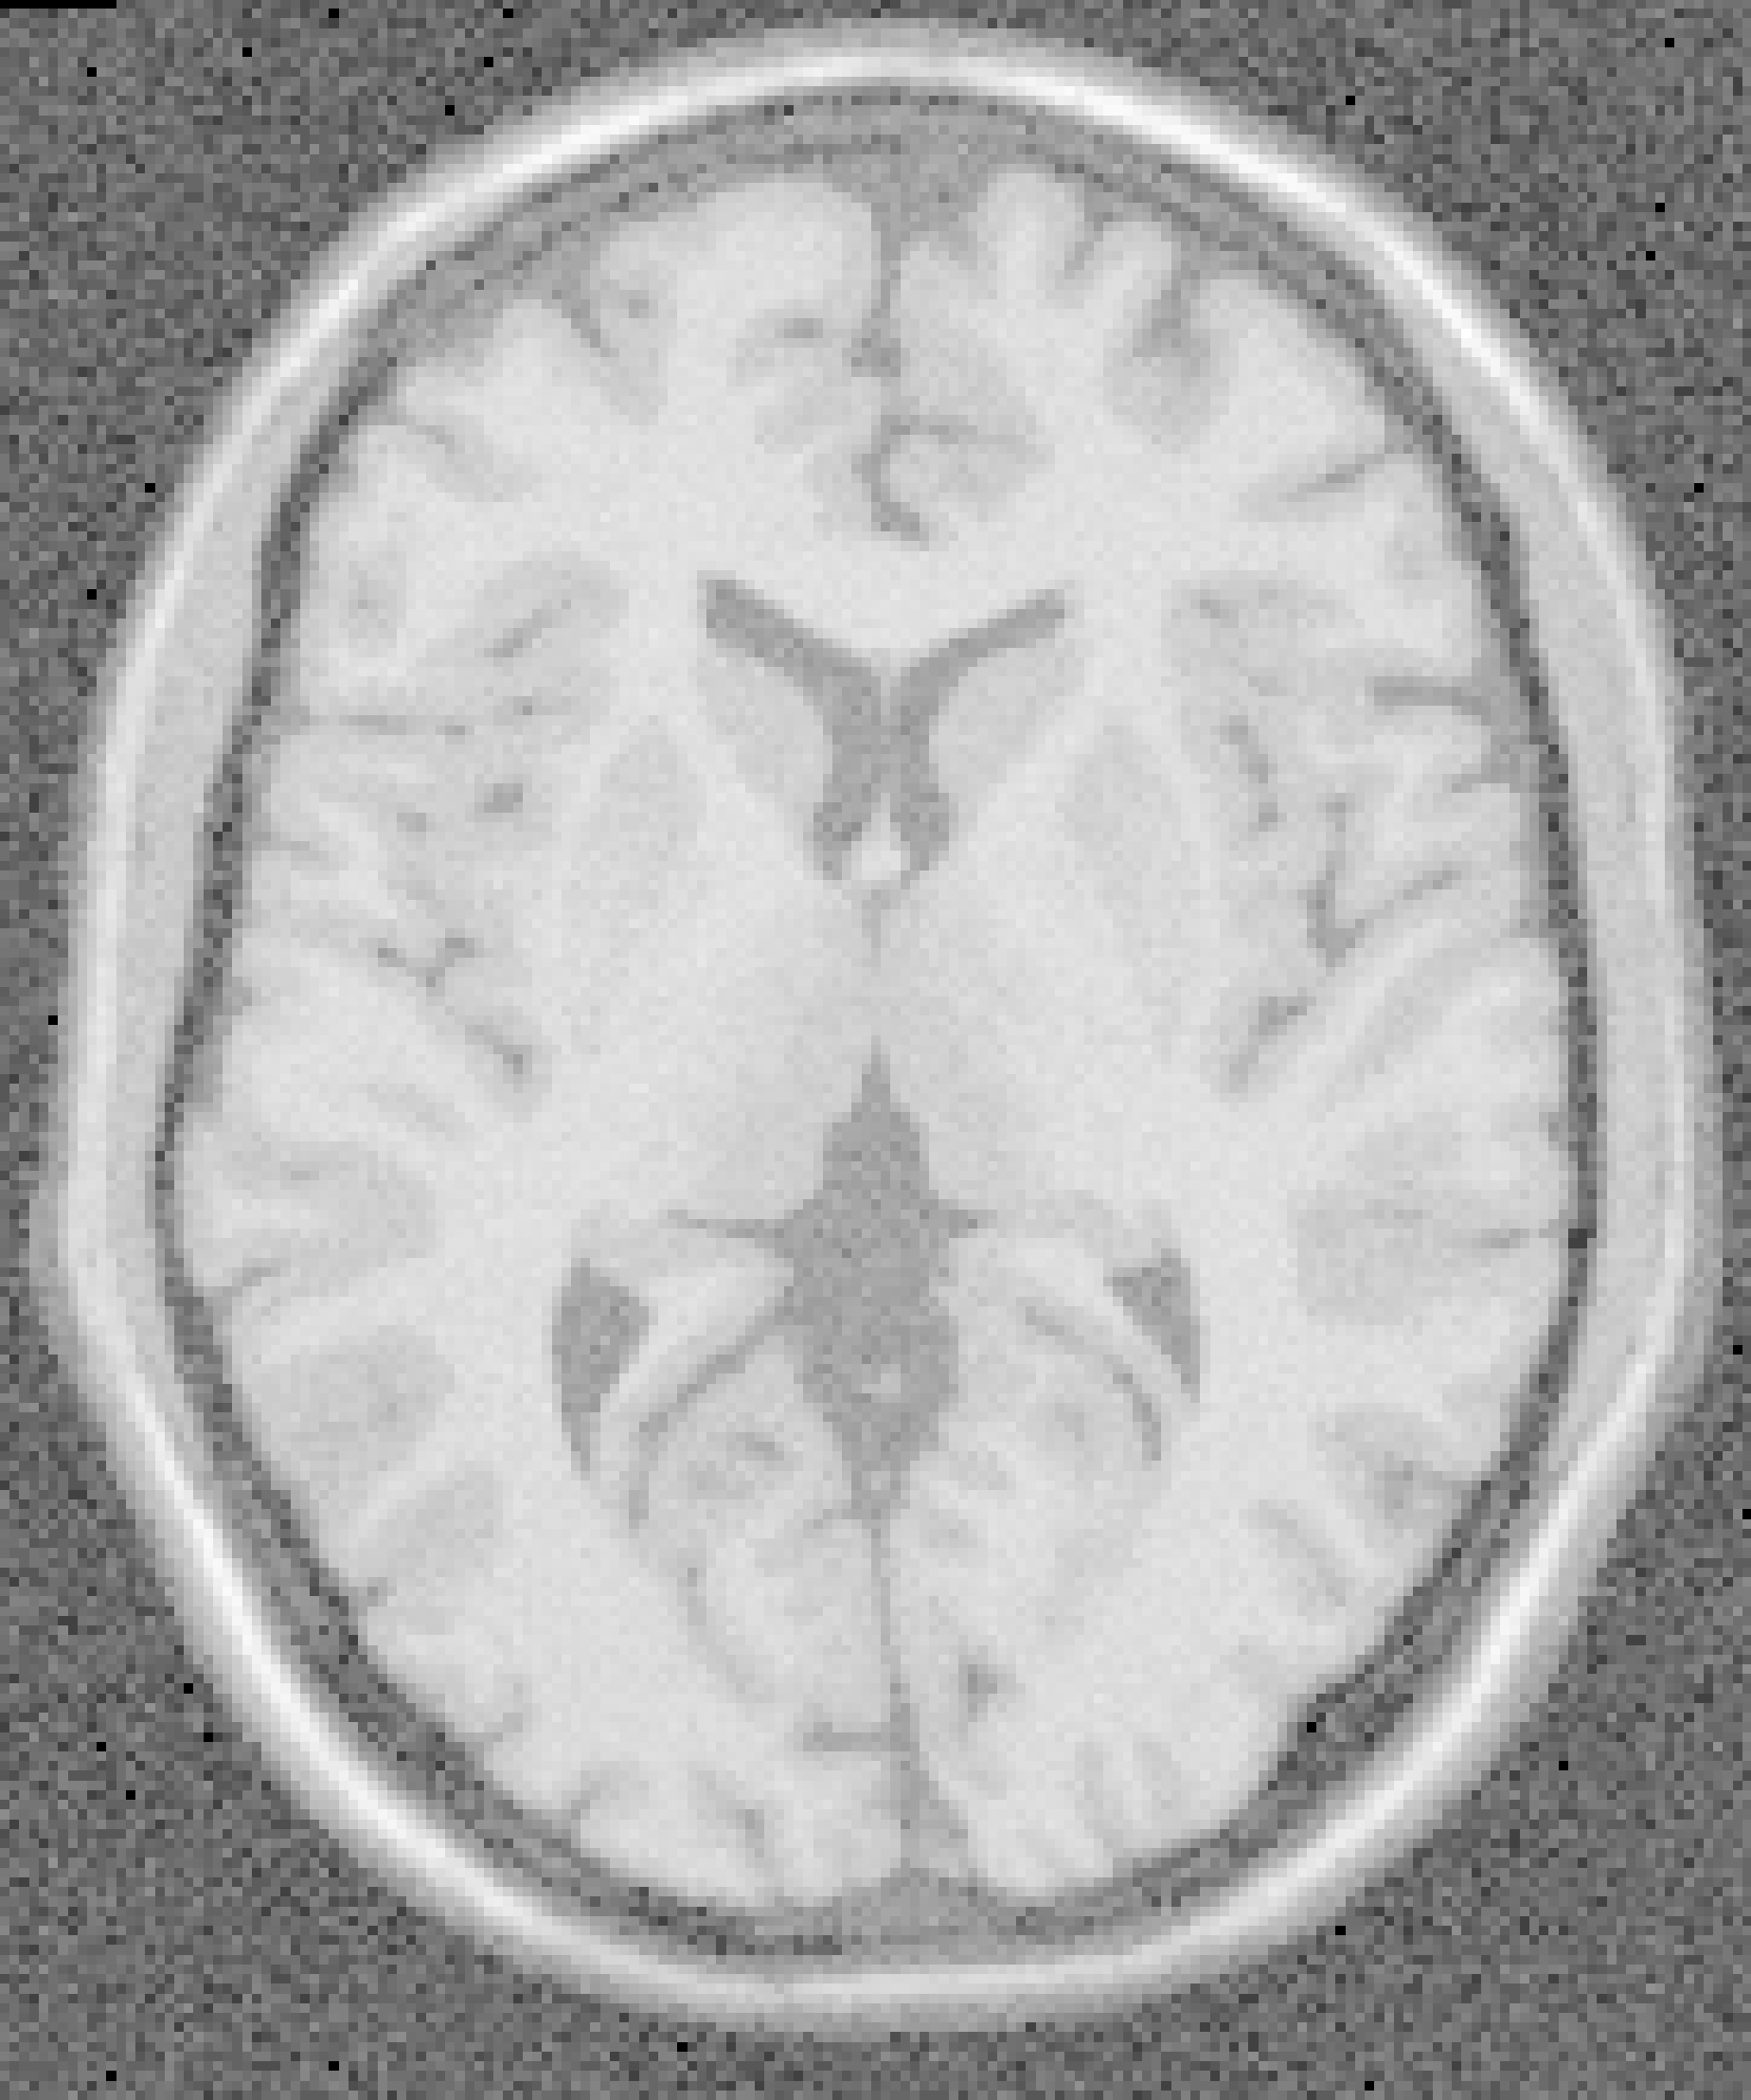
\includegraphics[width=\textwidth]{Figuras/ImageA_exp_gamma=0.25.png}
            \caption{$\gamma = 0.25$} 
         \end{subfigure}
         \begin{subfigure}[h]{0.2\textwidth}
            \centering
            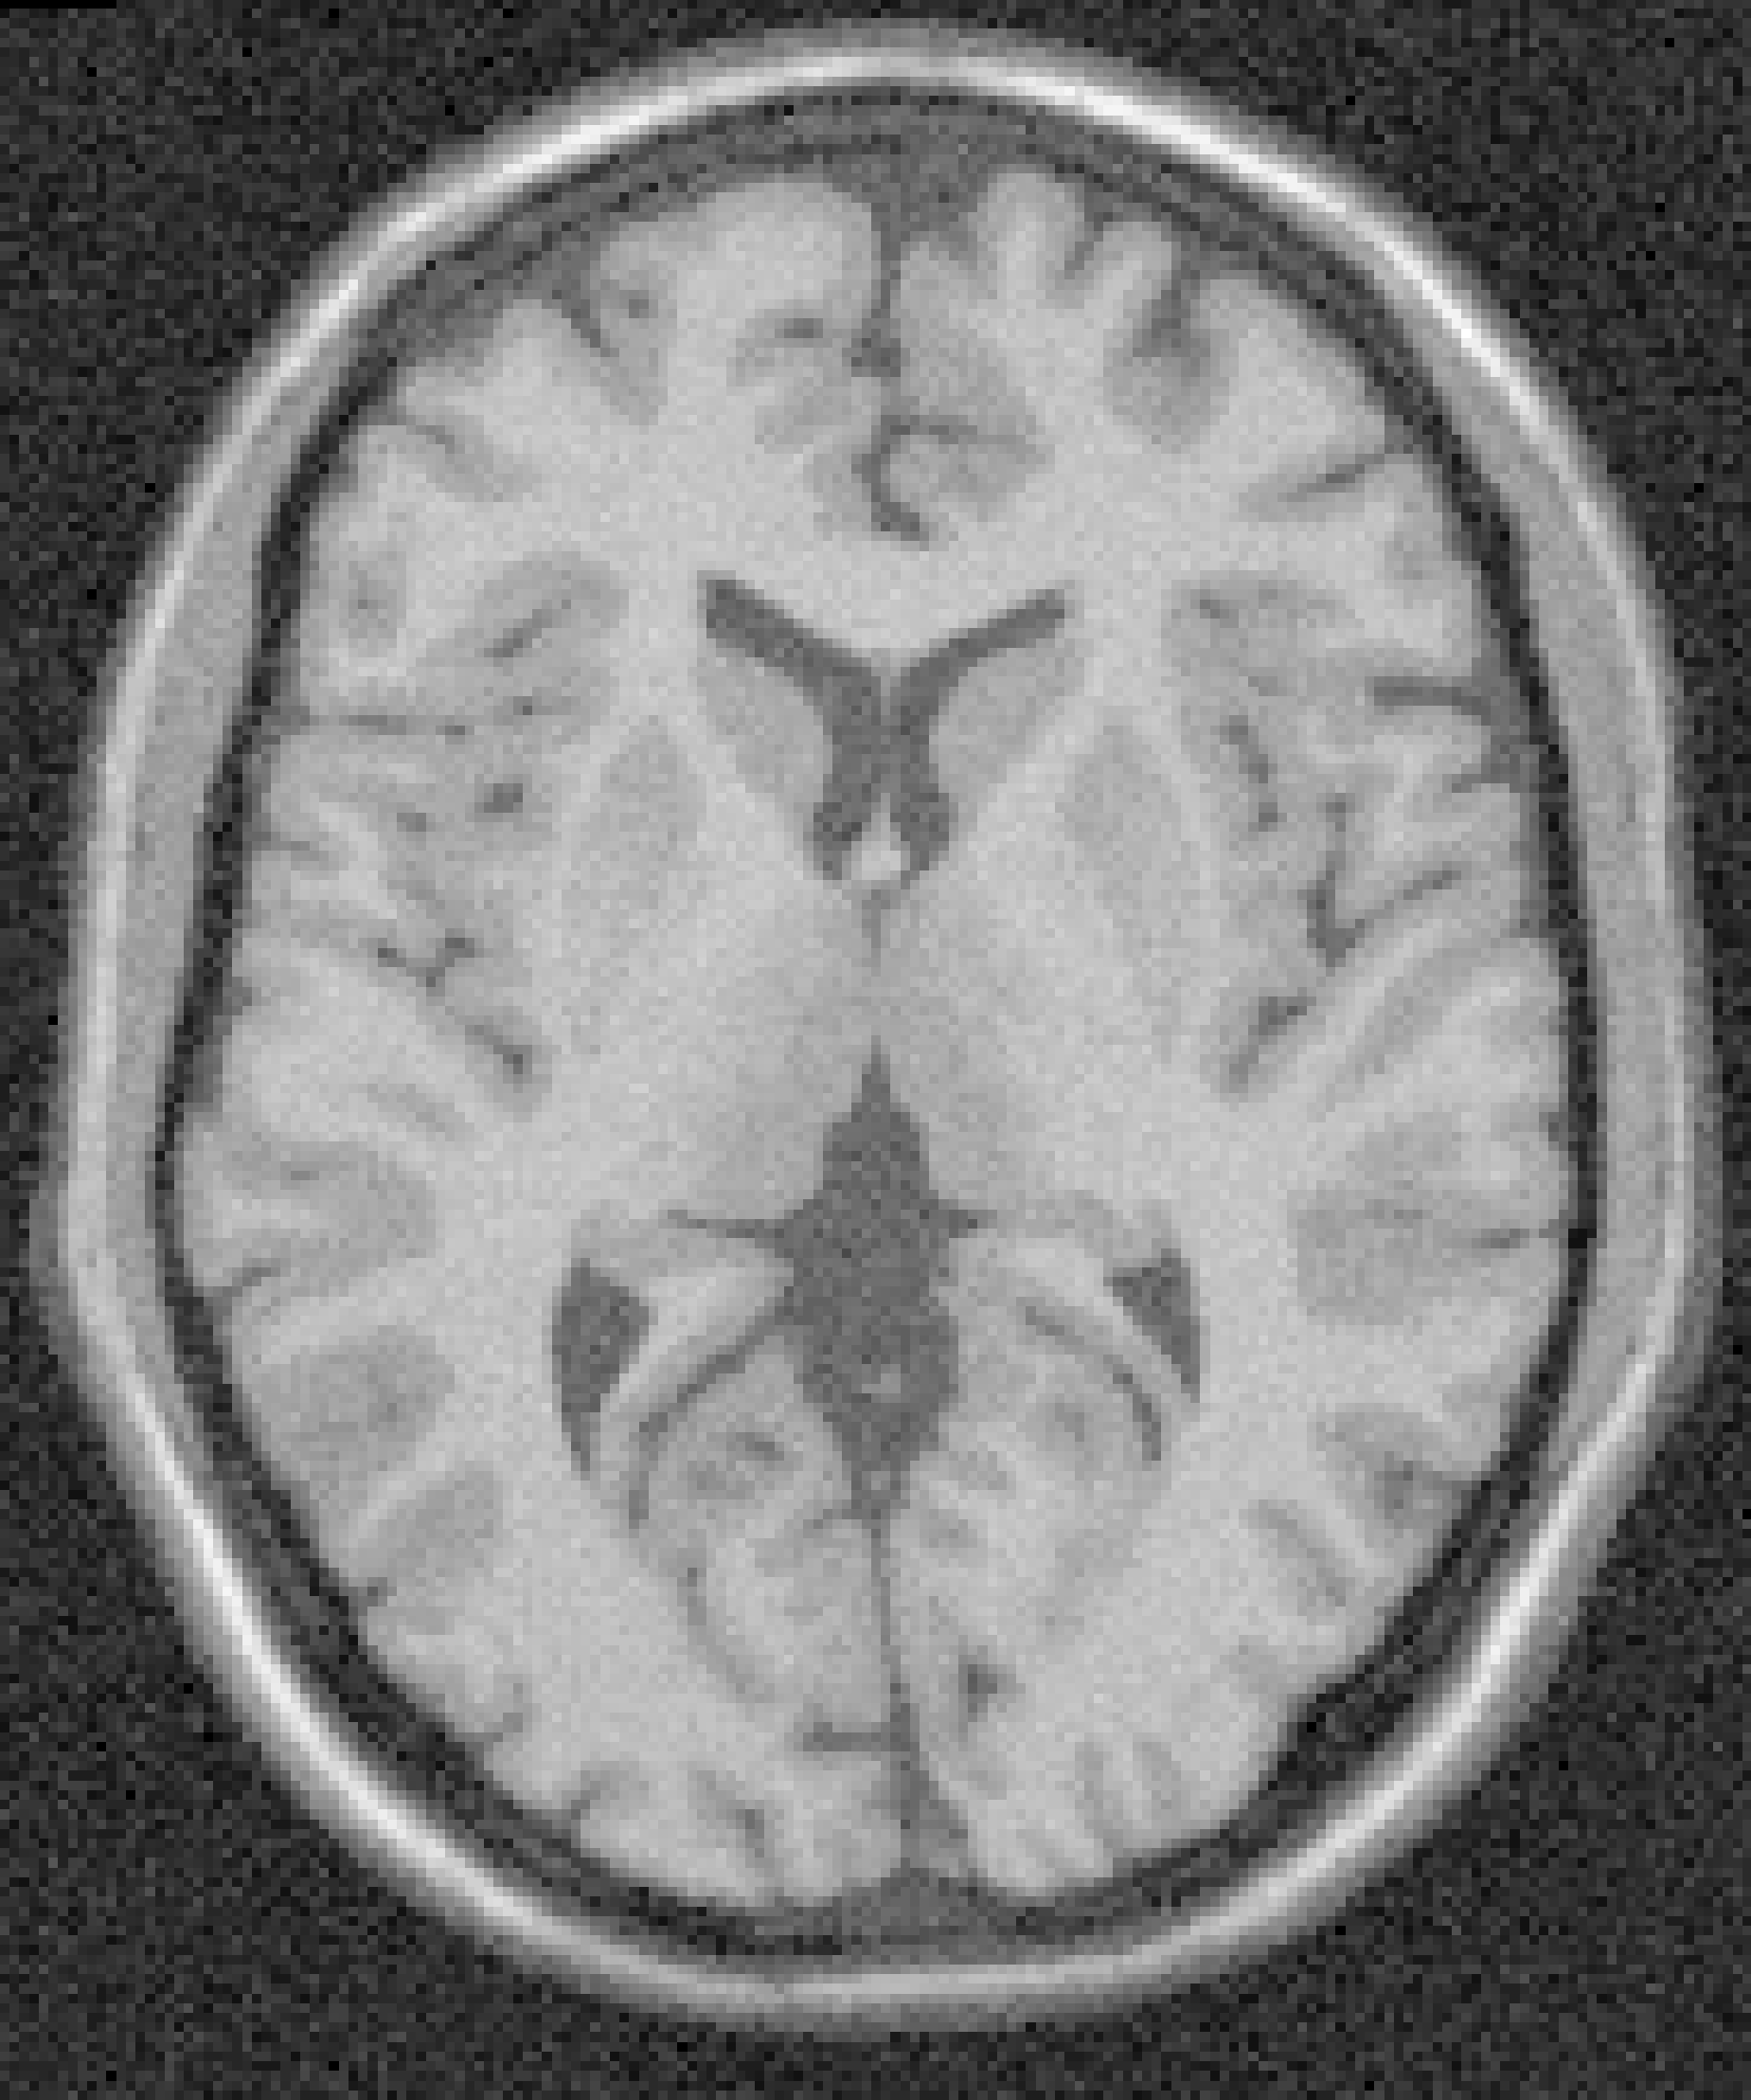
\includegraphics[width=\textwidth]{Figuras/ImageA_exp_gamma=0.5.png}
            \caption{$\gamma = 0.50$} 
         \end{subfigure}
         \begin{subfigure}[h]{0.2\textwidth}
            \centering
            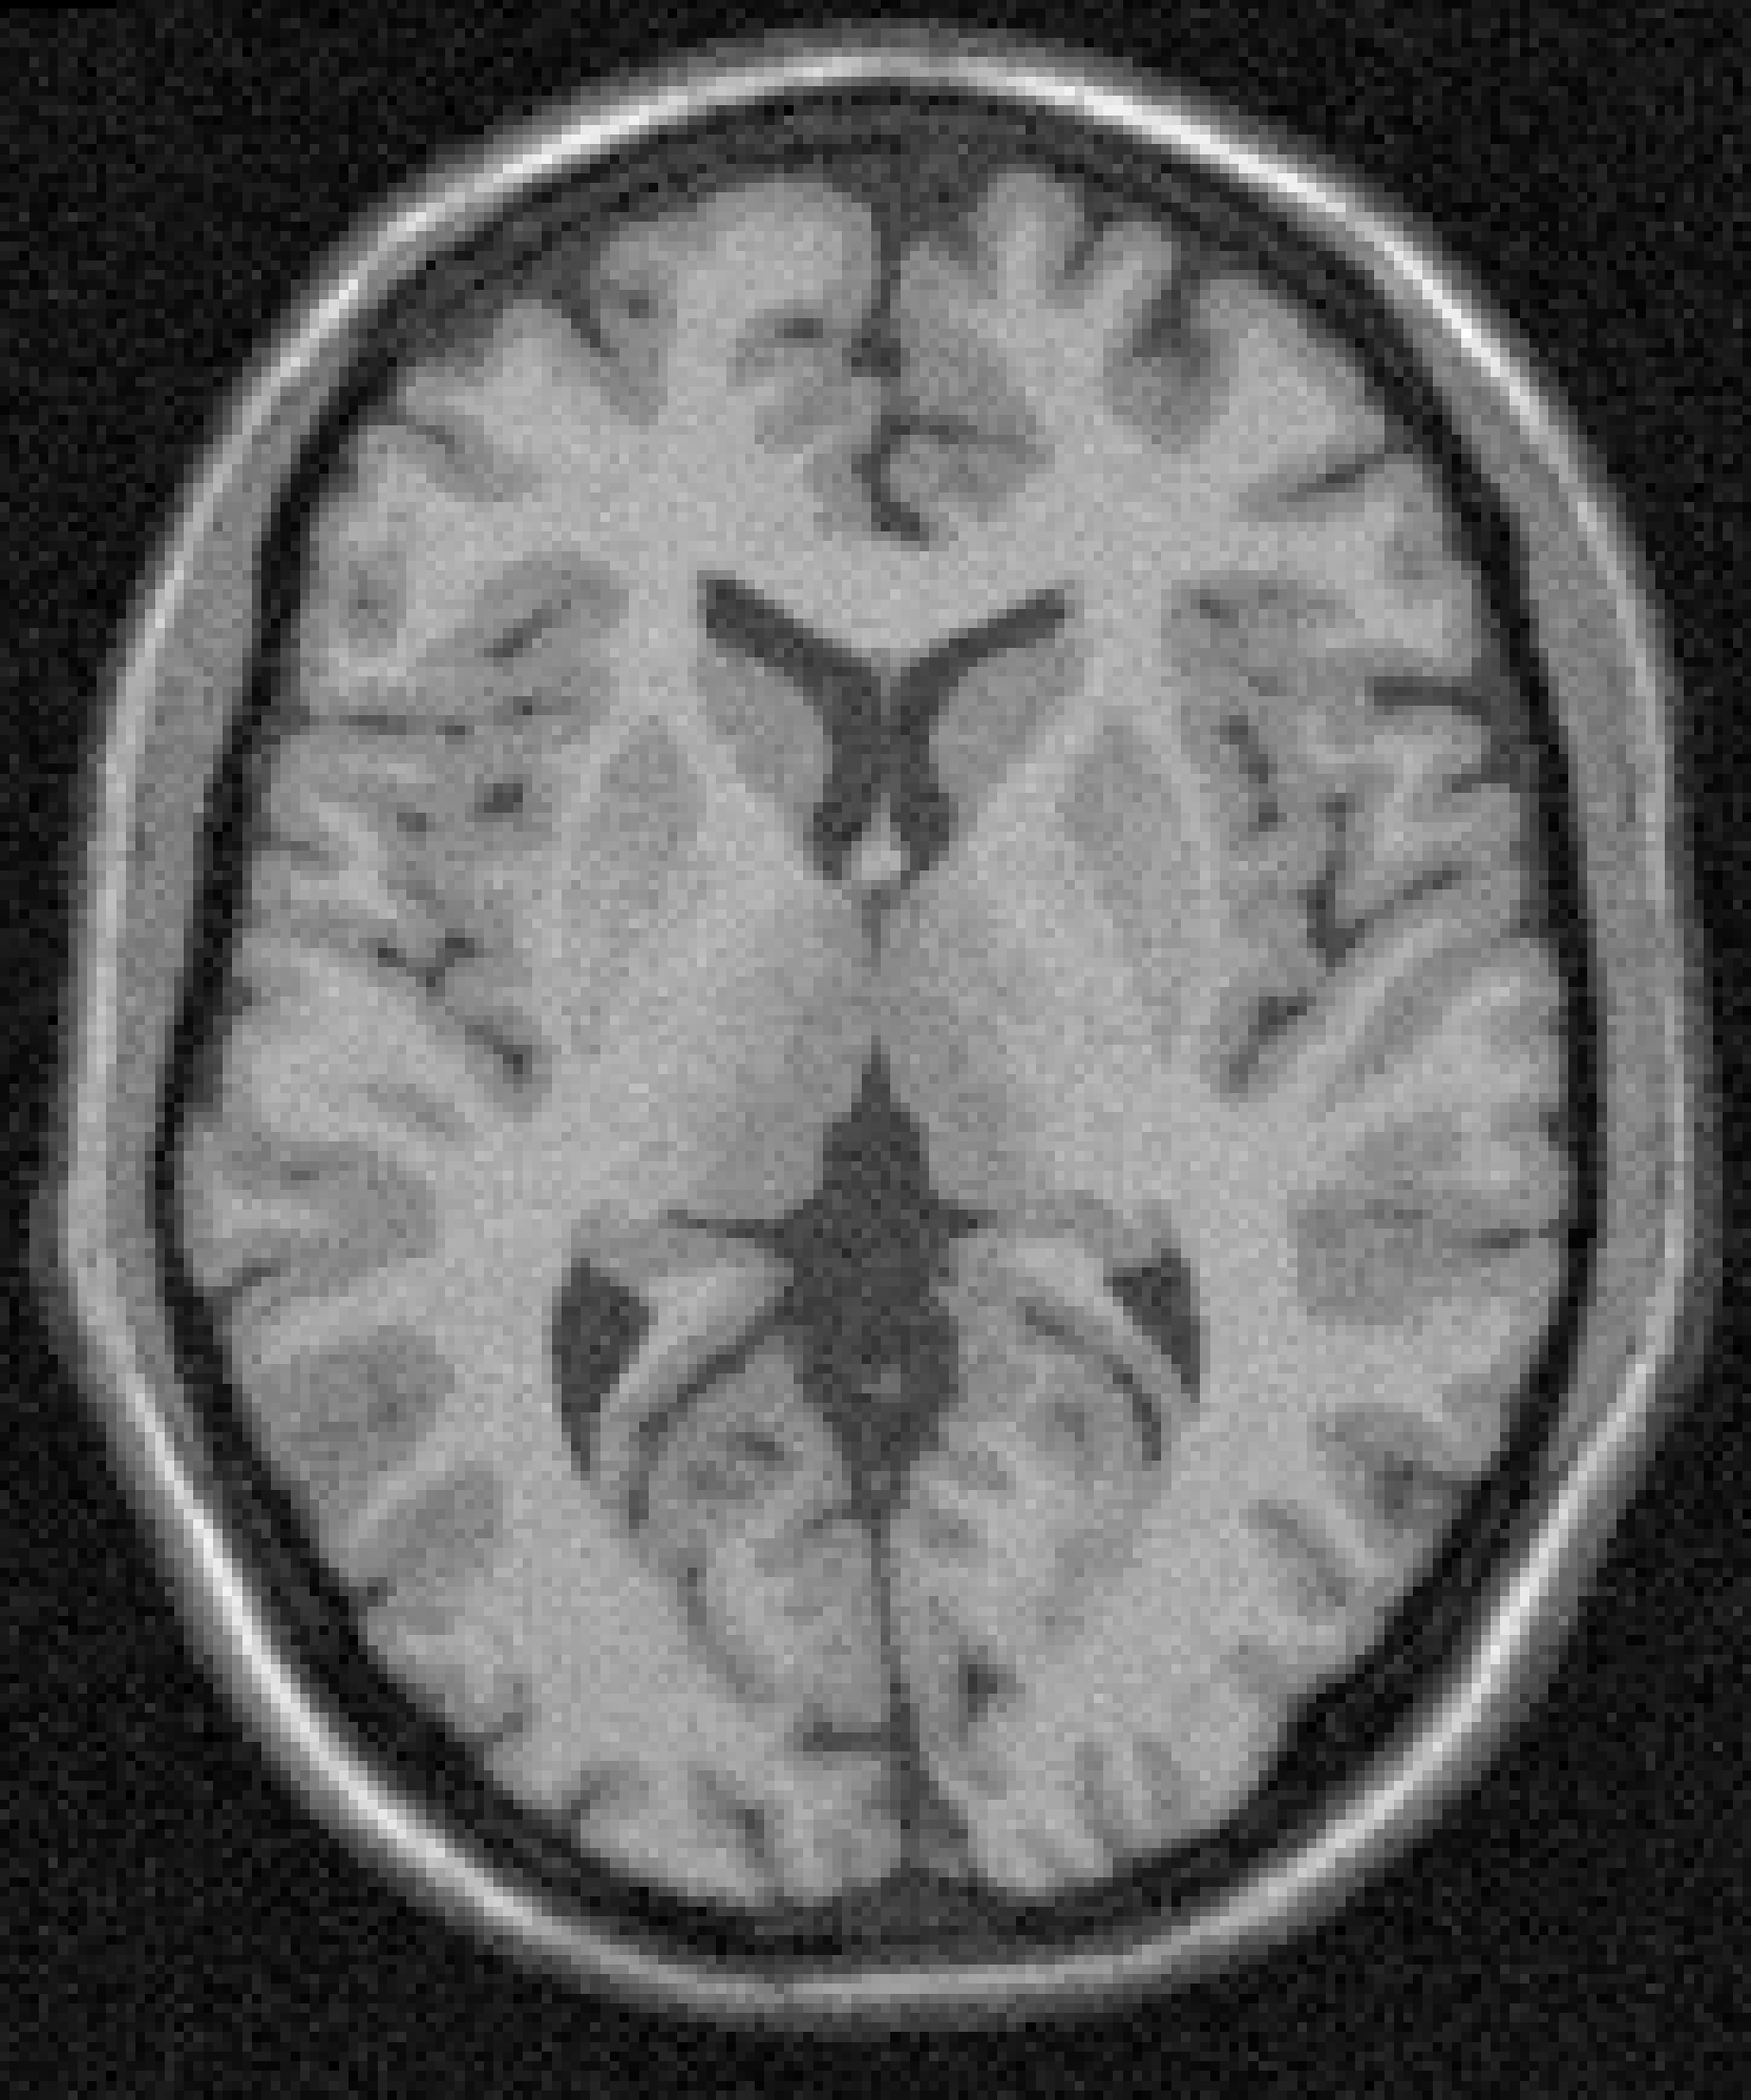
\includegraphics[width=\textwidth]{Figuras/ImageA_exp_gamma=0.75.png}
            \caption{$\gamma = 0.75$} 
         \end{subfigure}
         \\
         \begin{subfigure}[h]{0.2\textwidth}
            \centering
            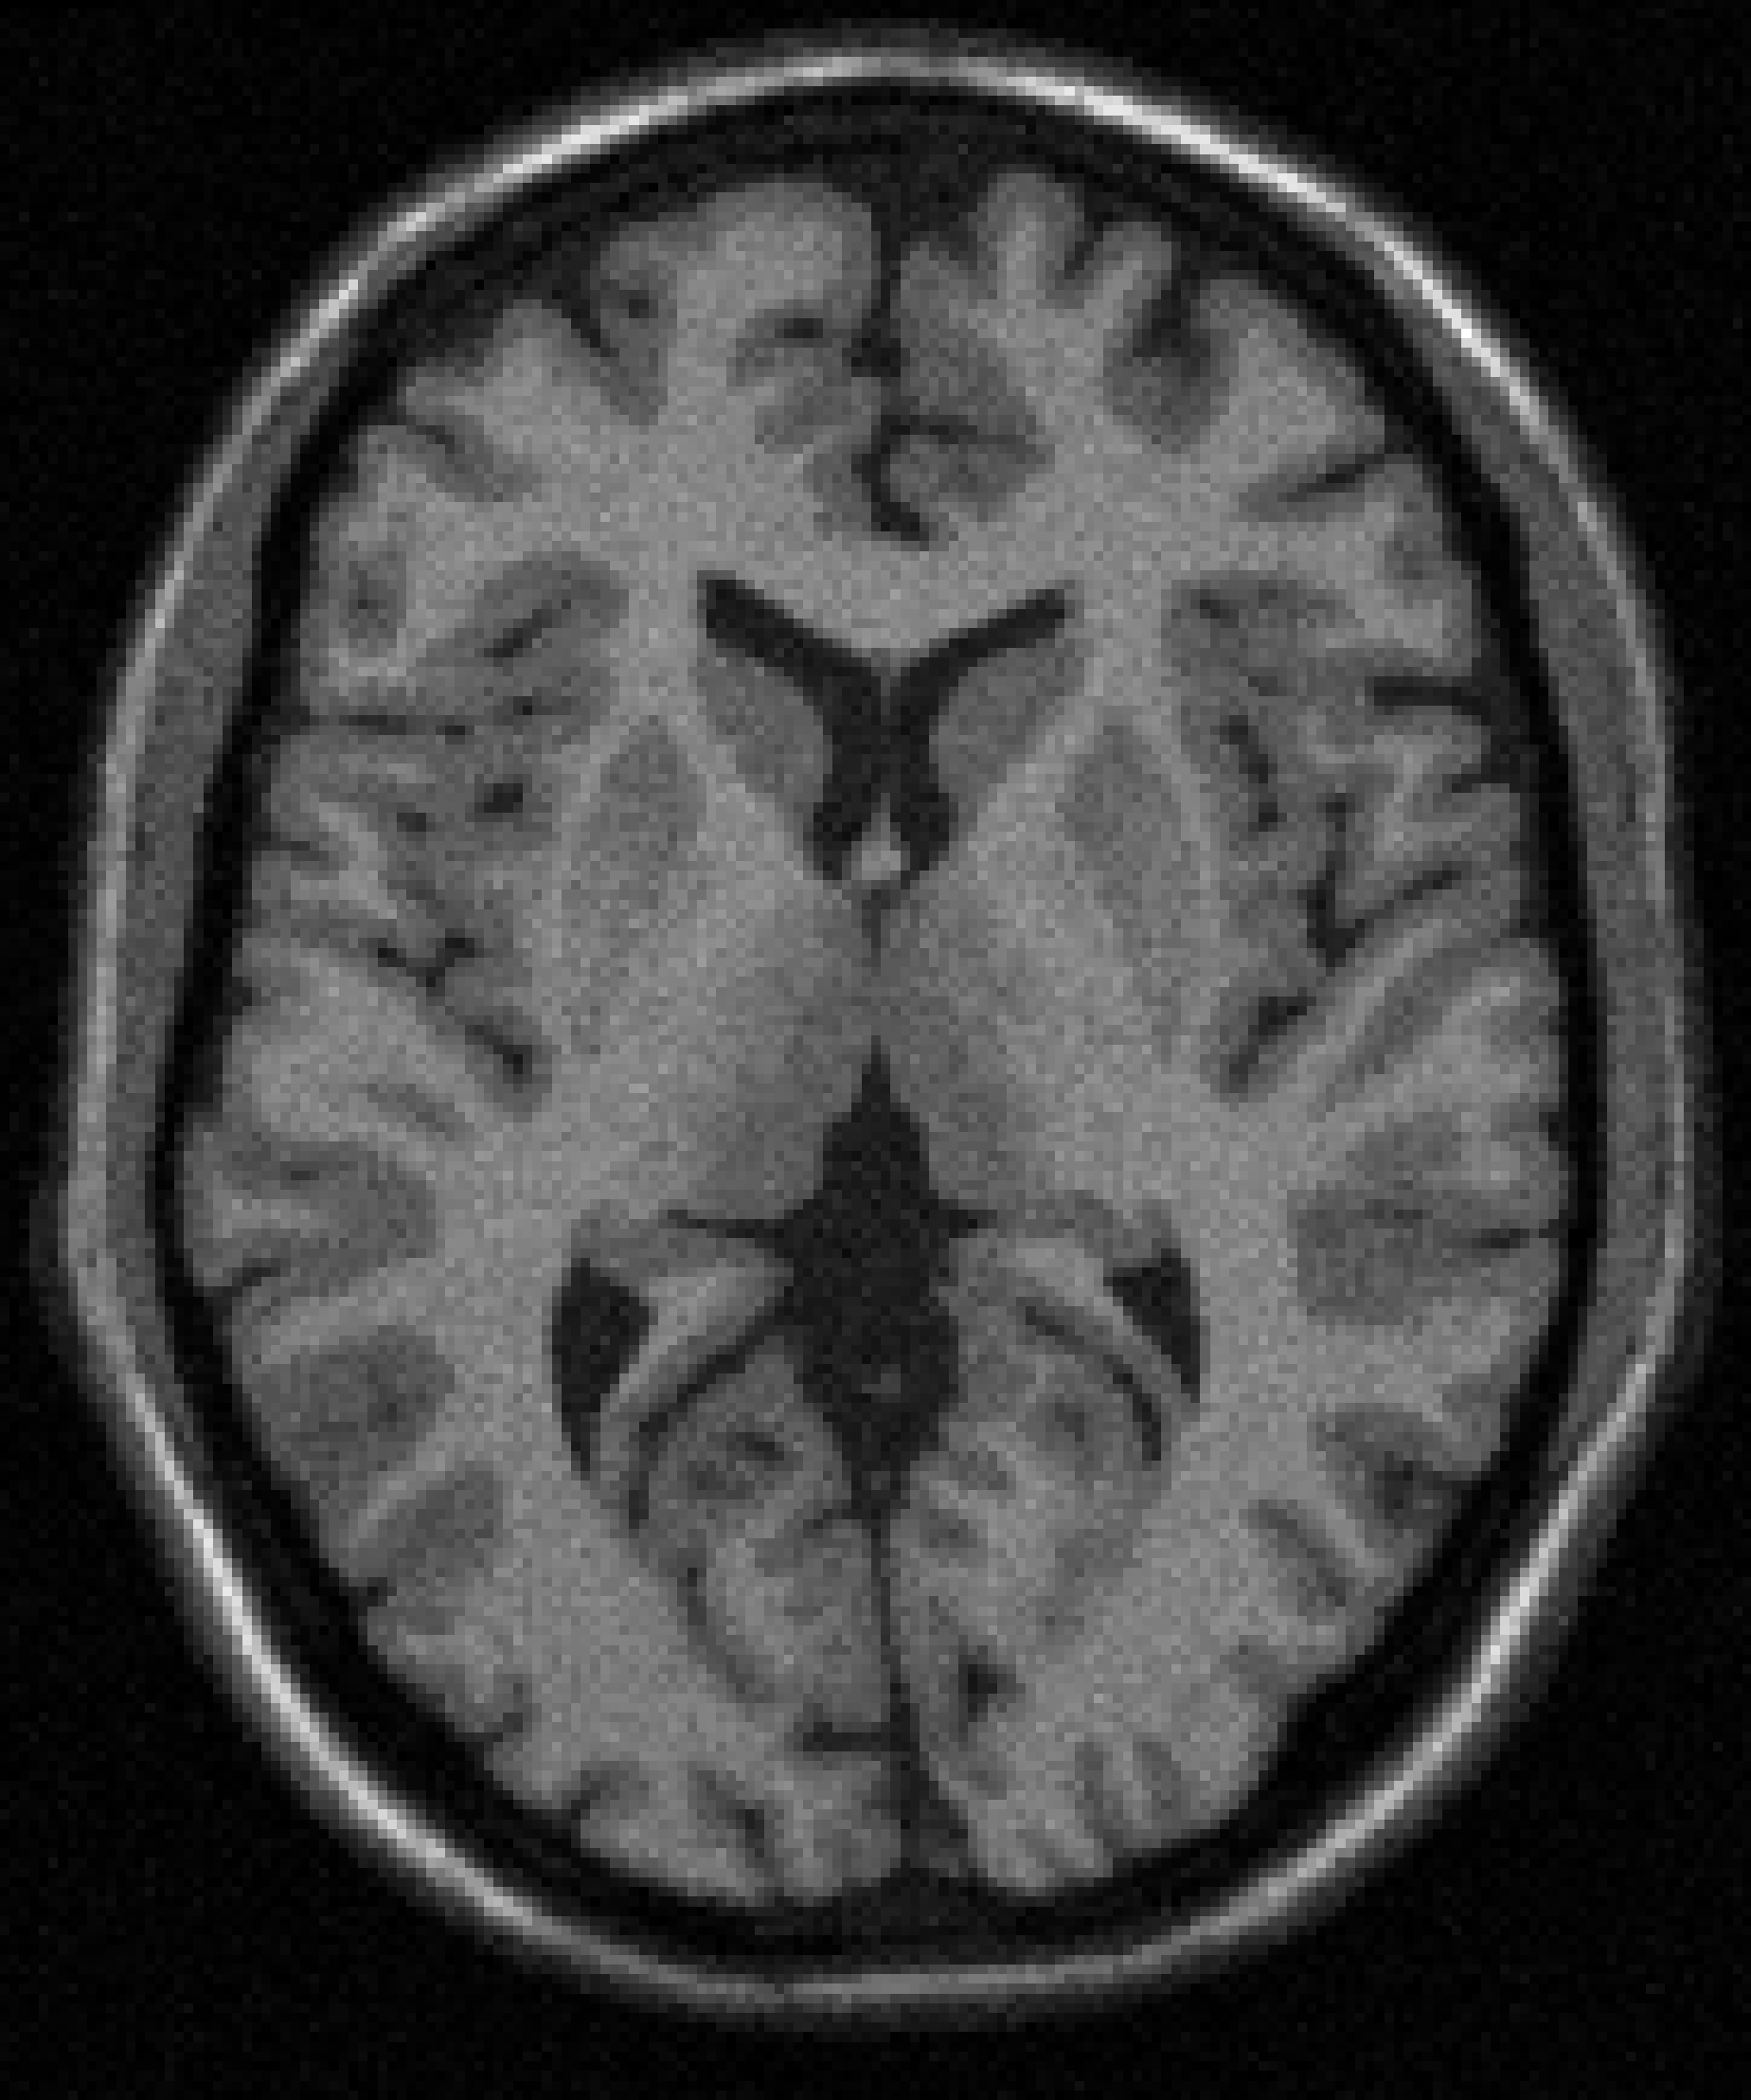
\includegraphics[width=\textwidth]{Figuras/ImageA_exp_gamma=1.25.png}
            \caption{$\gamma = 1.25$} 
         \end{subfigure}
         \begin{subfigure}[h]{0.2\textwidth}
            \centering
            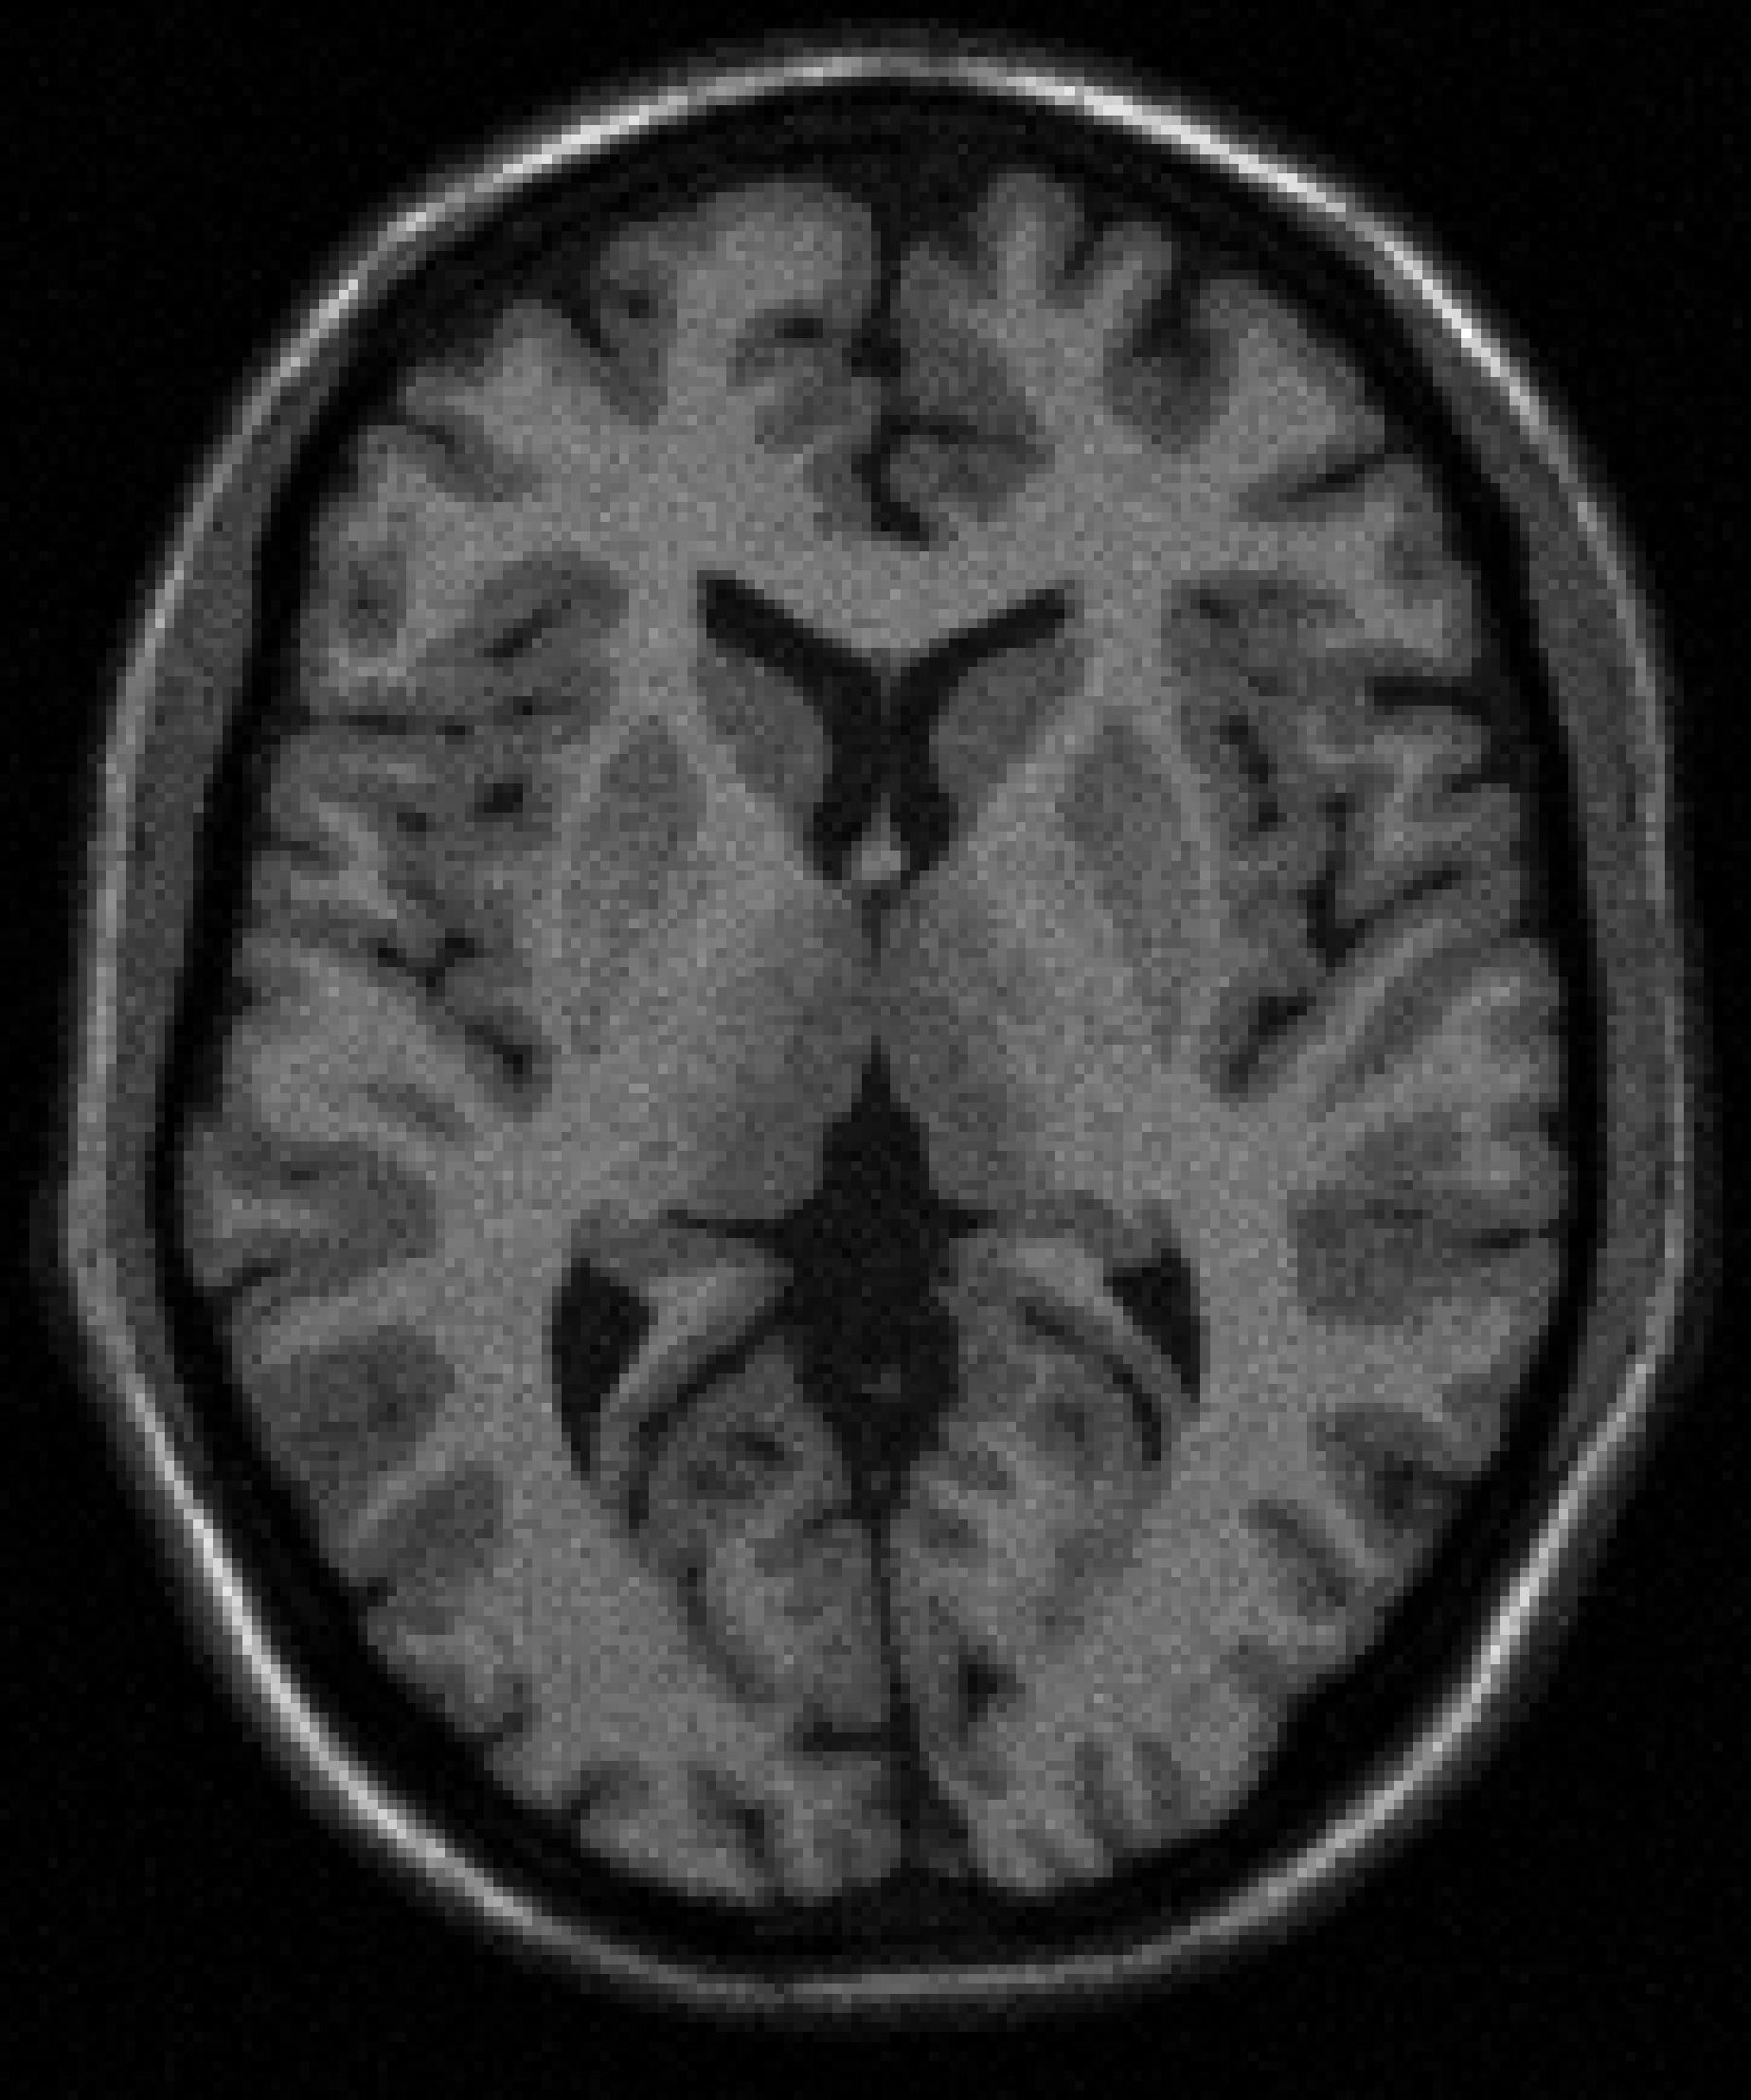
\includegraphics[width=\textwidth]{Figuras/ImageA_exp_gamma=1.5.png}
            \caption{$\gamma = 1.5$} 
         \end{subfigure}
         \begin{subfigure}[h]{0.2\textwidth}
            \centering
            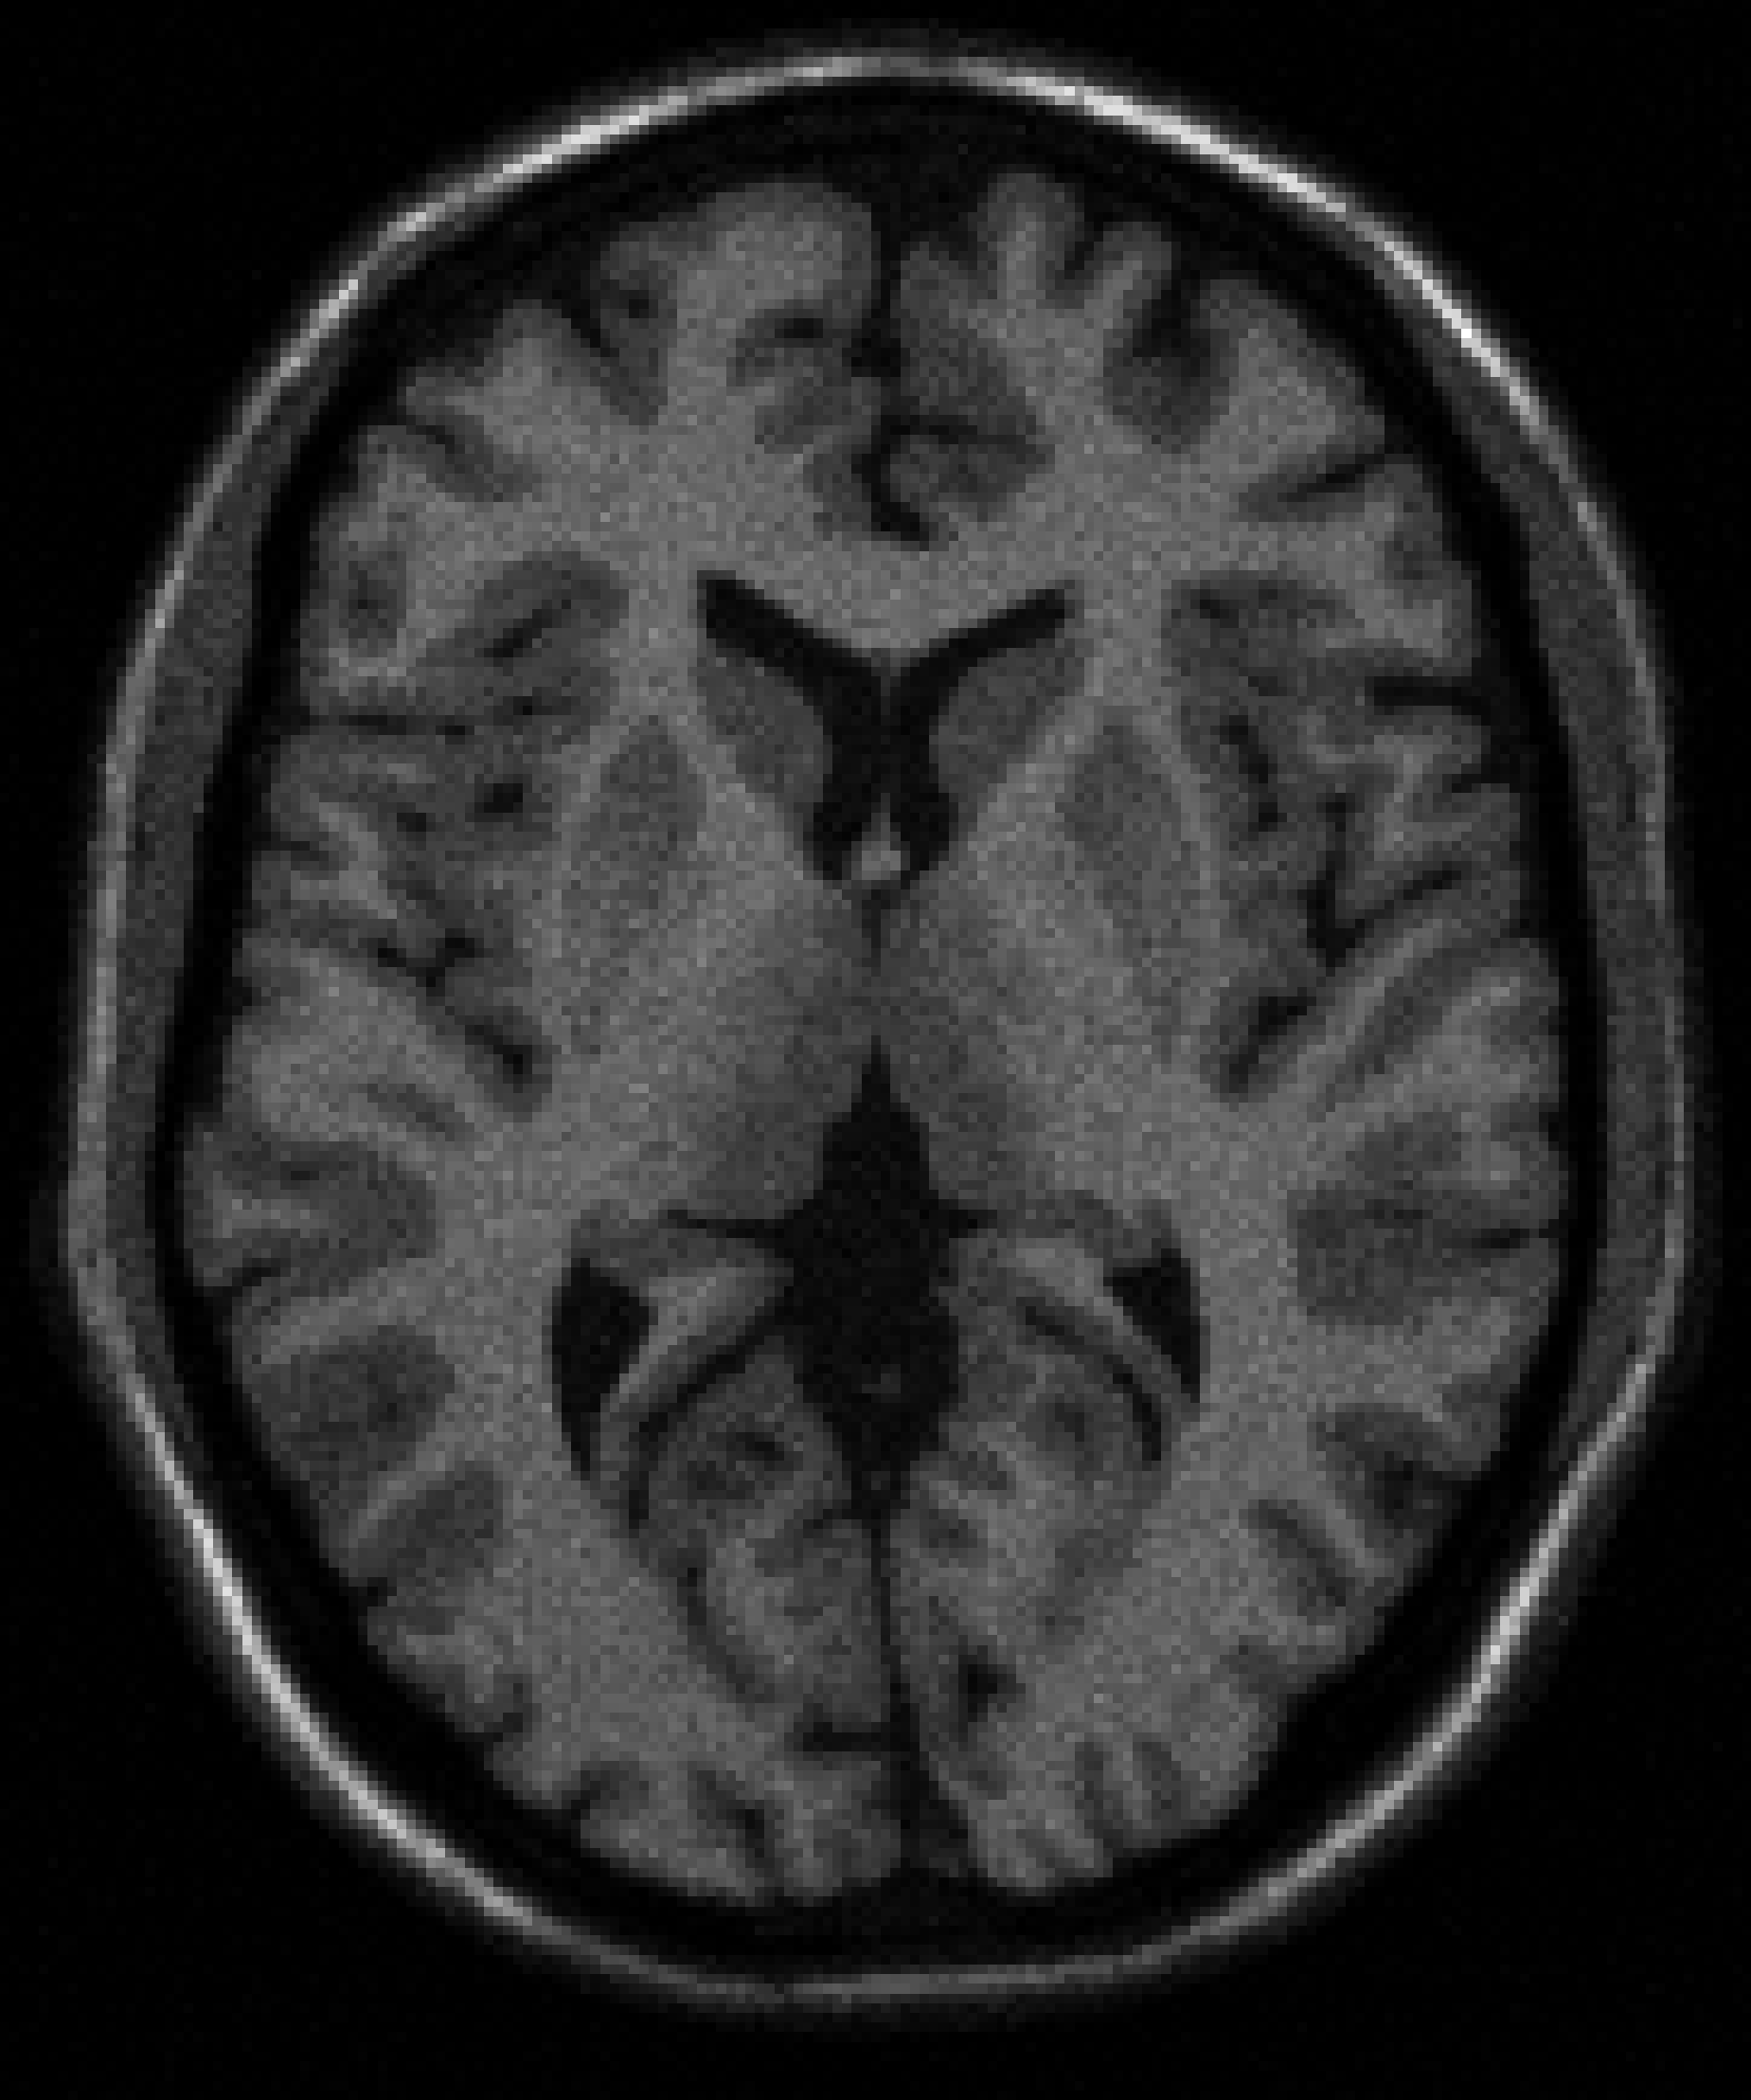
\includegraphics[width=\textwidth]{Figuras/ImageA_exp_gamma=1.75.png}
            \caption{$\gamma = 1.75$} 
         \end{subfigure}
    \caption{Transformación $\gamma$ aplicada a la imagenA original.}
    \label{fig:Exptrans}
\end{figure}

Por último, en las Figs. \ref{fig:EQ_sustraction}, \ref{fig:binary_sustraction}, \ref{fig:Exptrans0.5_sustraction} y \ref{fig:Exptrans1.75_sustraction} se muestran la resta de la imagenA original con la imagenA luego de aplicarle transformaciones de ecualización, binarización y $\gamma$ con $\gamma = 0.5,1.75$ respectivamente.

\begin{figure}[H]
    \centering
        \begin{subfigure}[h]{0.3\textwidth}
            \centering
            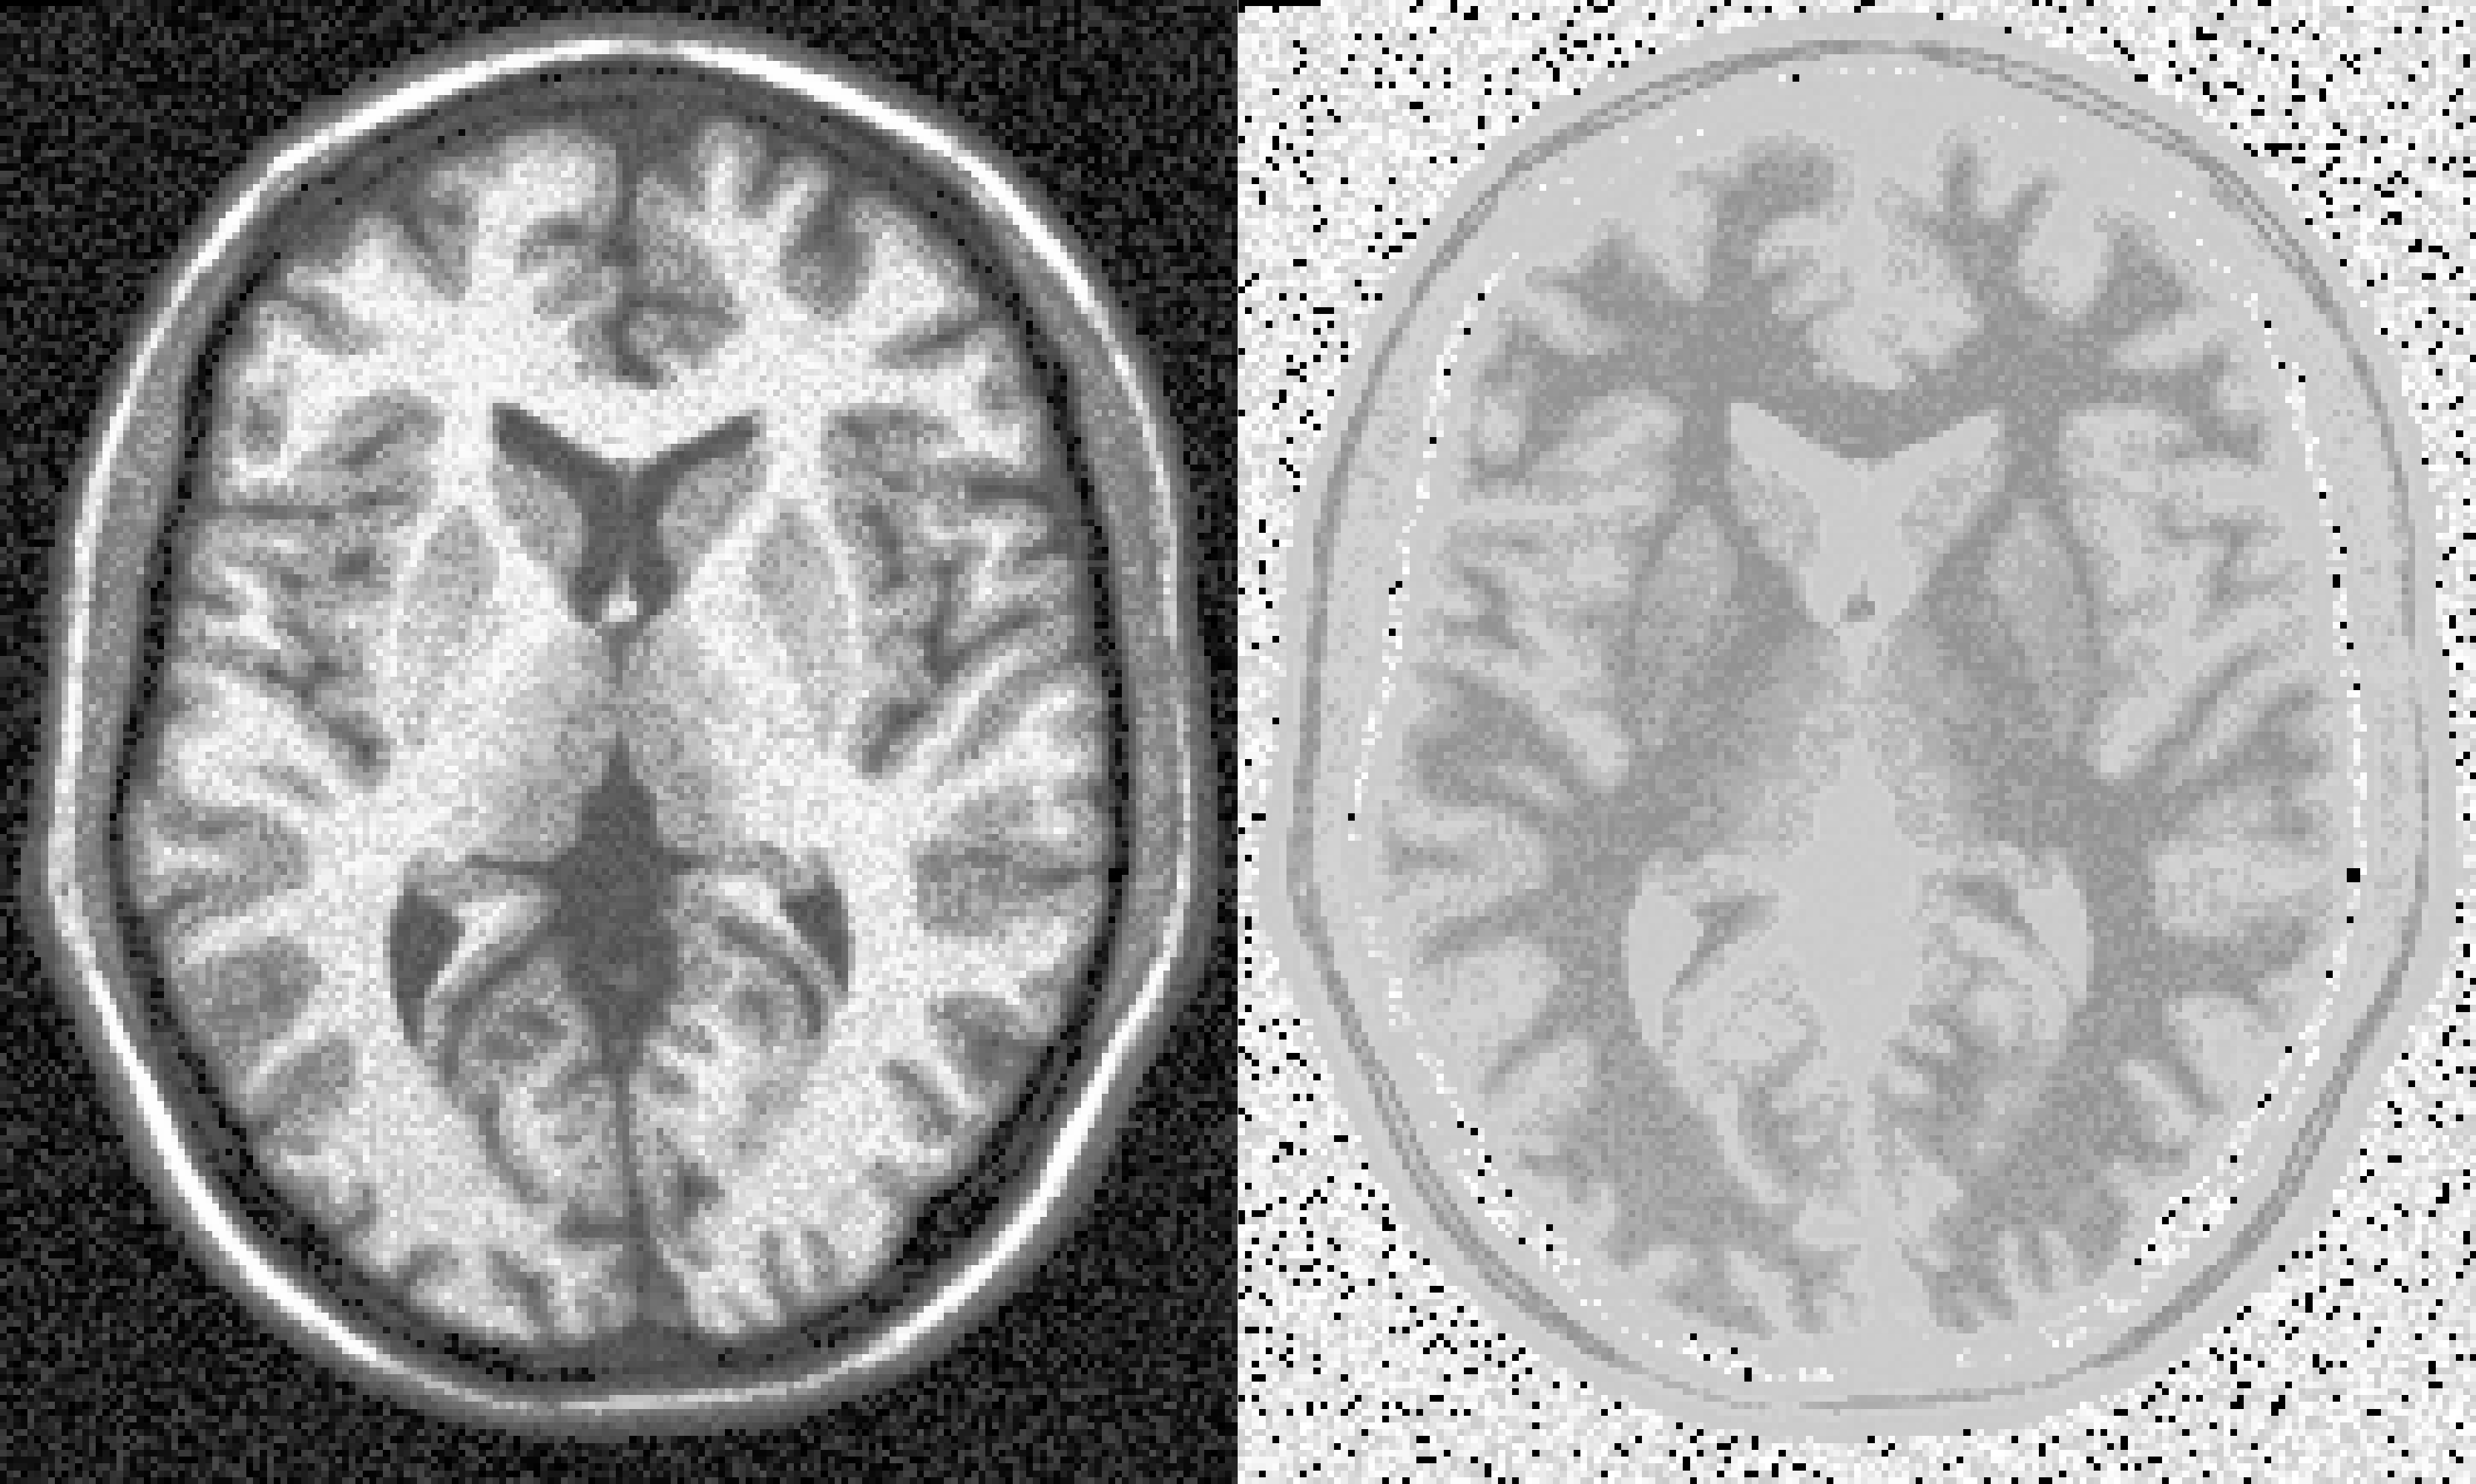
\includegraphics[width=\textwidth]{Figuras/dif_EQ.png}                
            \caption{Ecualización.}
            \label{fig:EQ_sustraction}
        \end{subfigure}
        \begin{subfigure}[h]{0.3\textwidth}
            \centering
            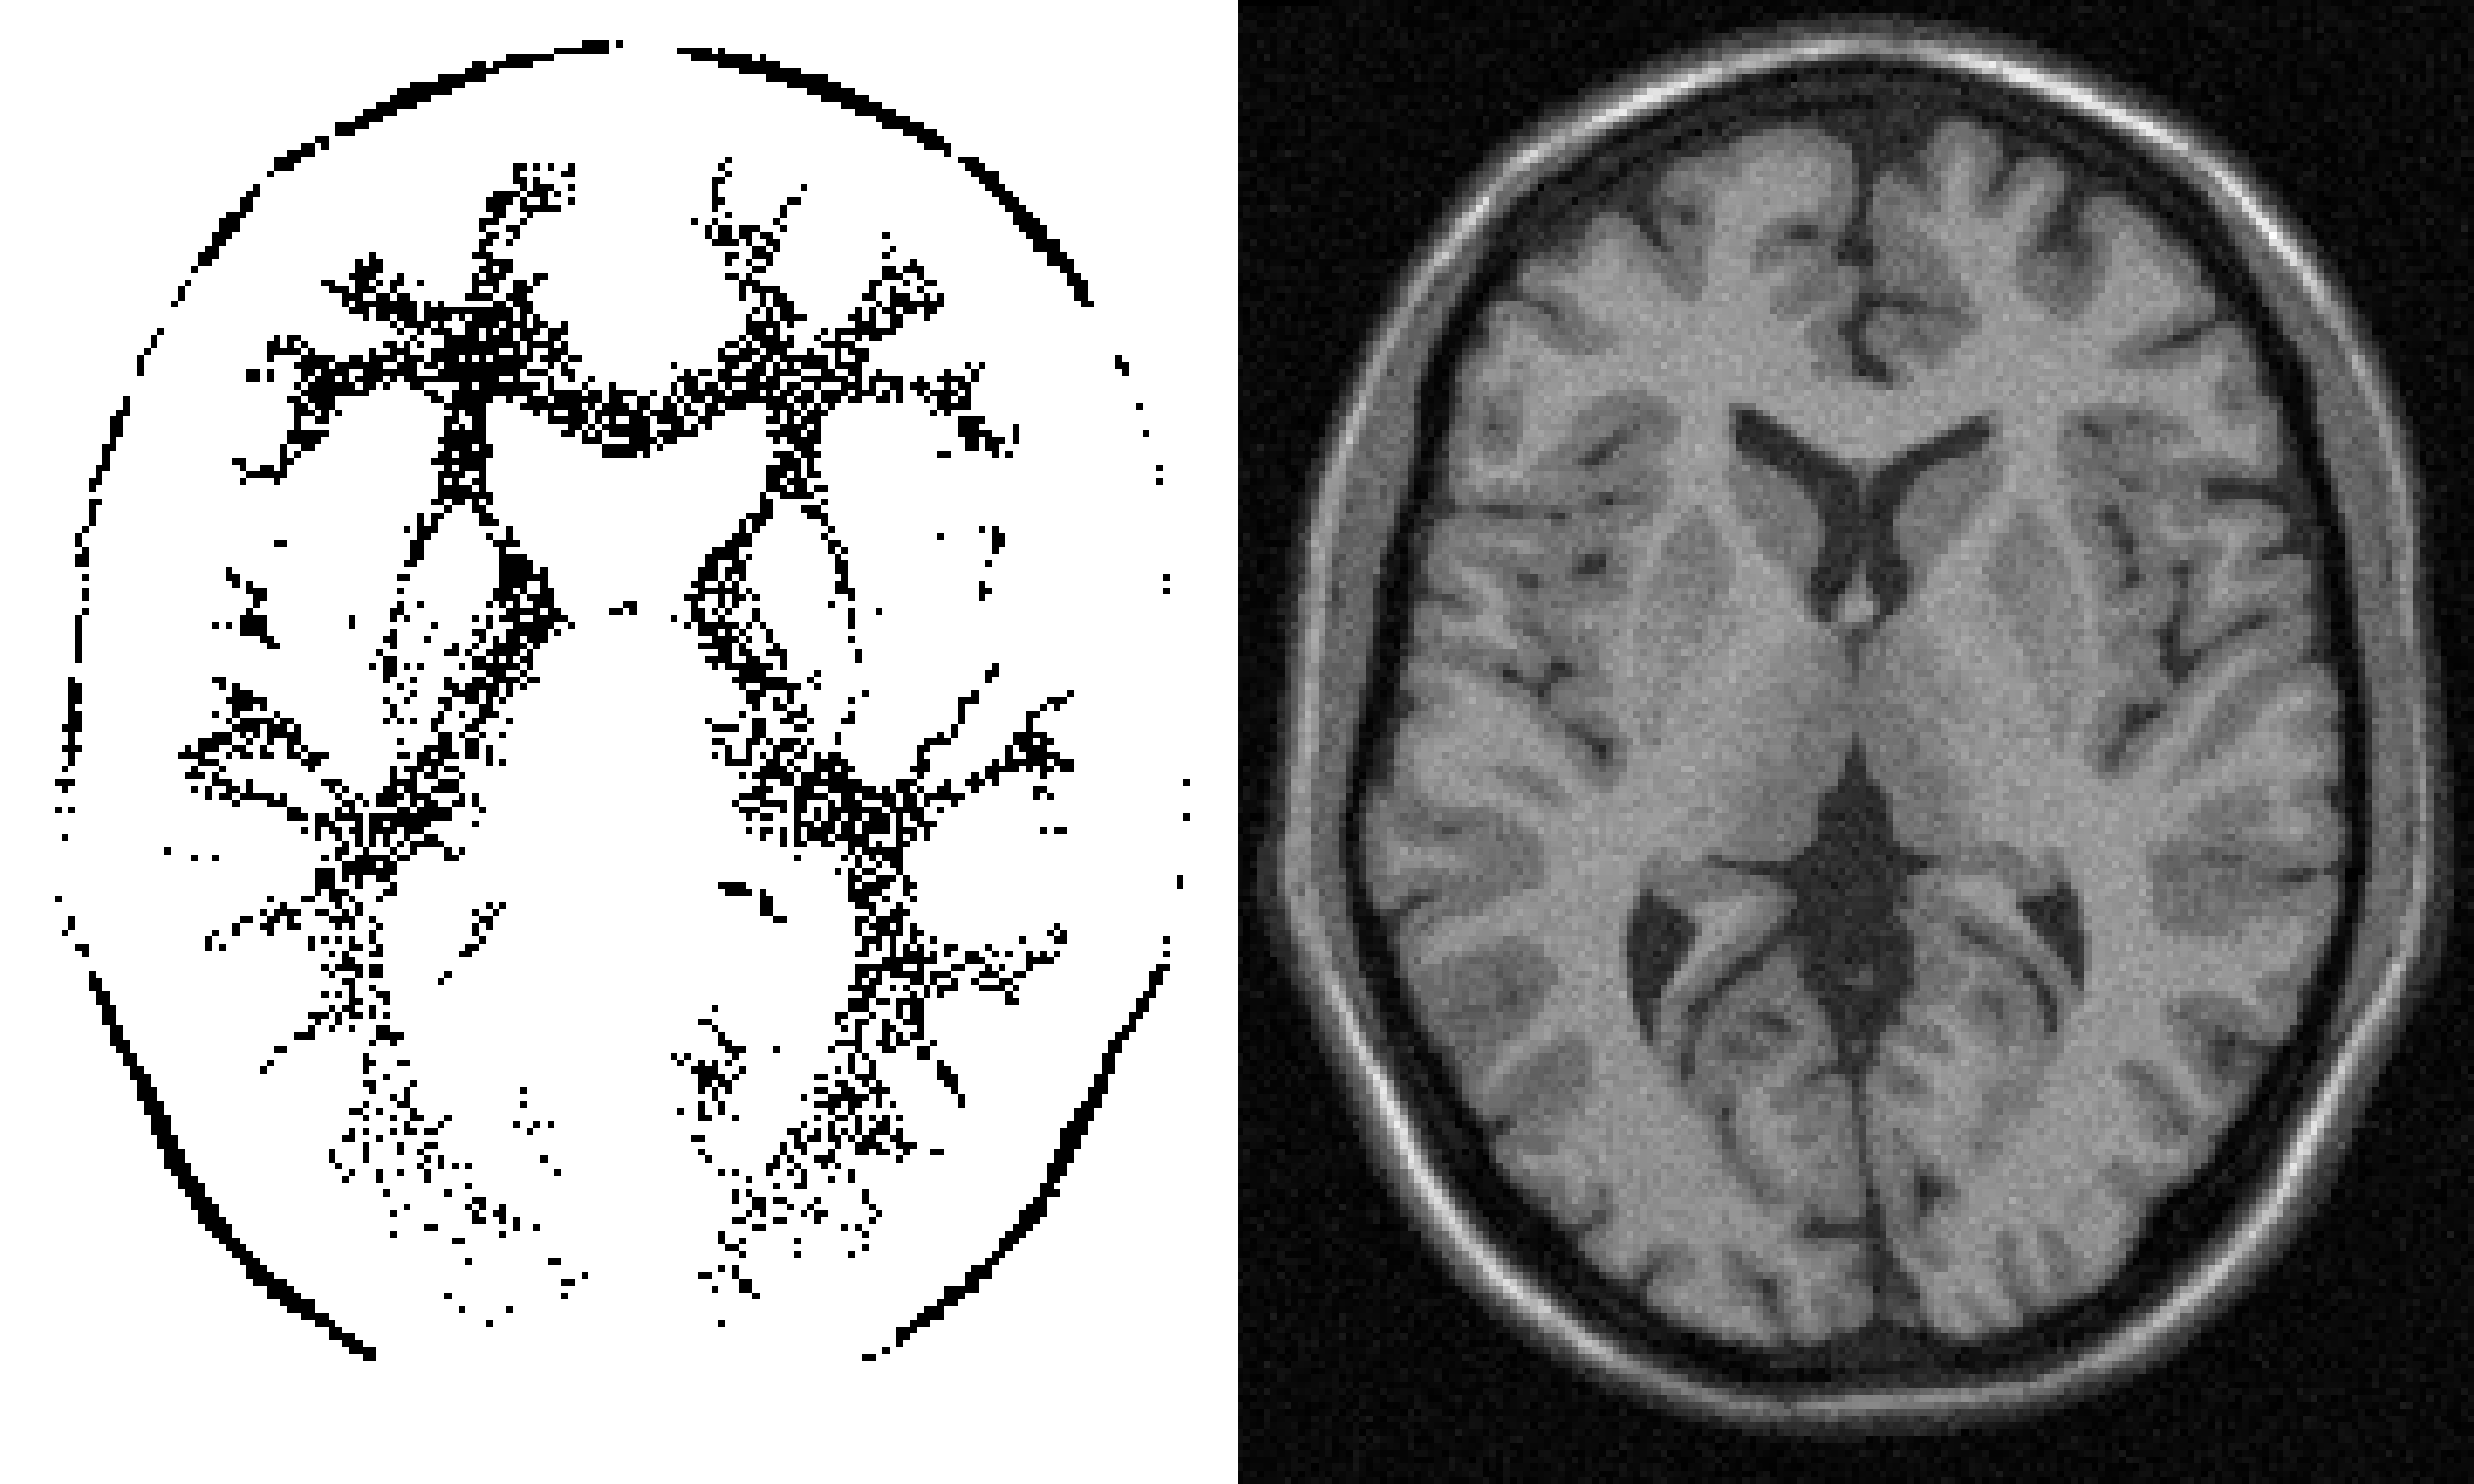
\includegraphics[width=\textwidth]{Figuras/dif_binary.png}
            \caption{Transformación binaria.} 
            \label{fig:binary_sustraction}
        \end{subfigure}
         \\
        \begin{subfigure}[h]{0.3\textwidth}
            \centering
            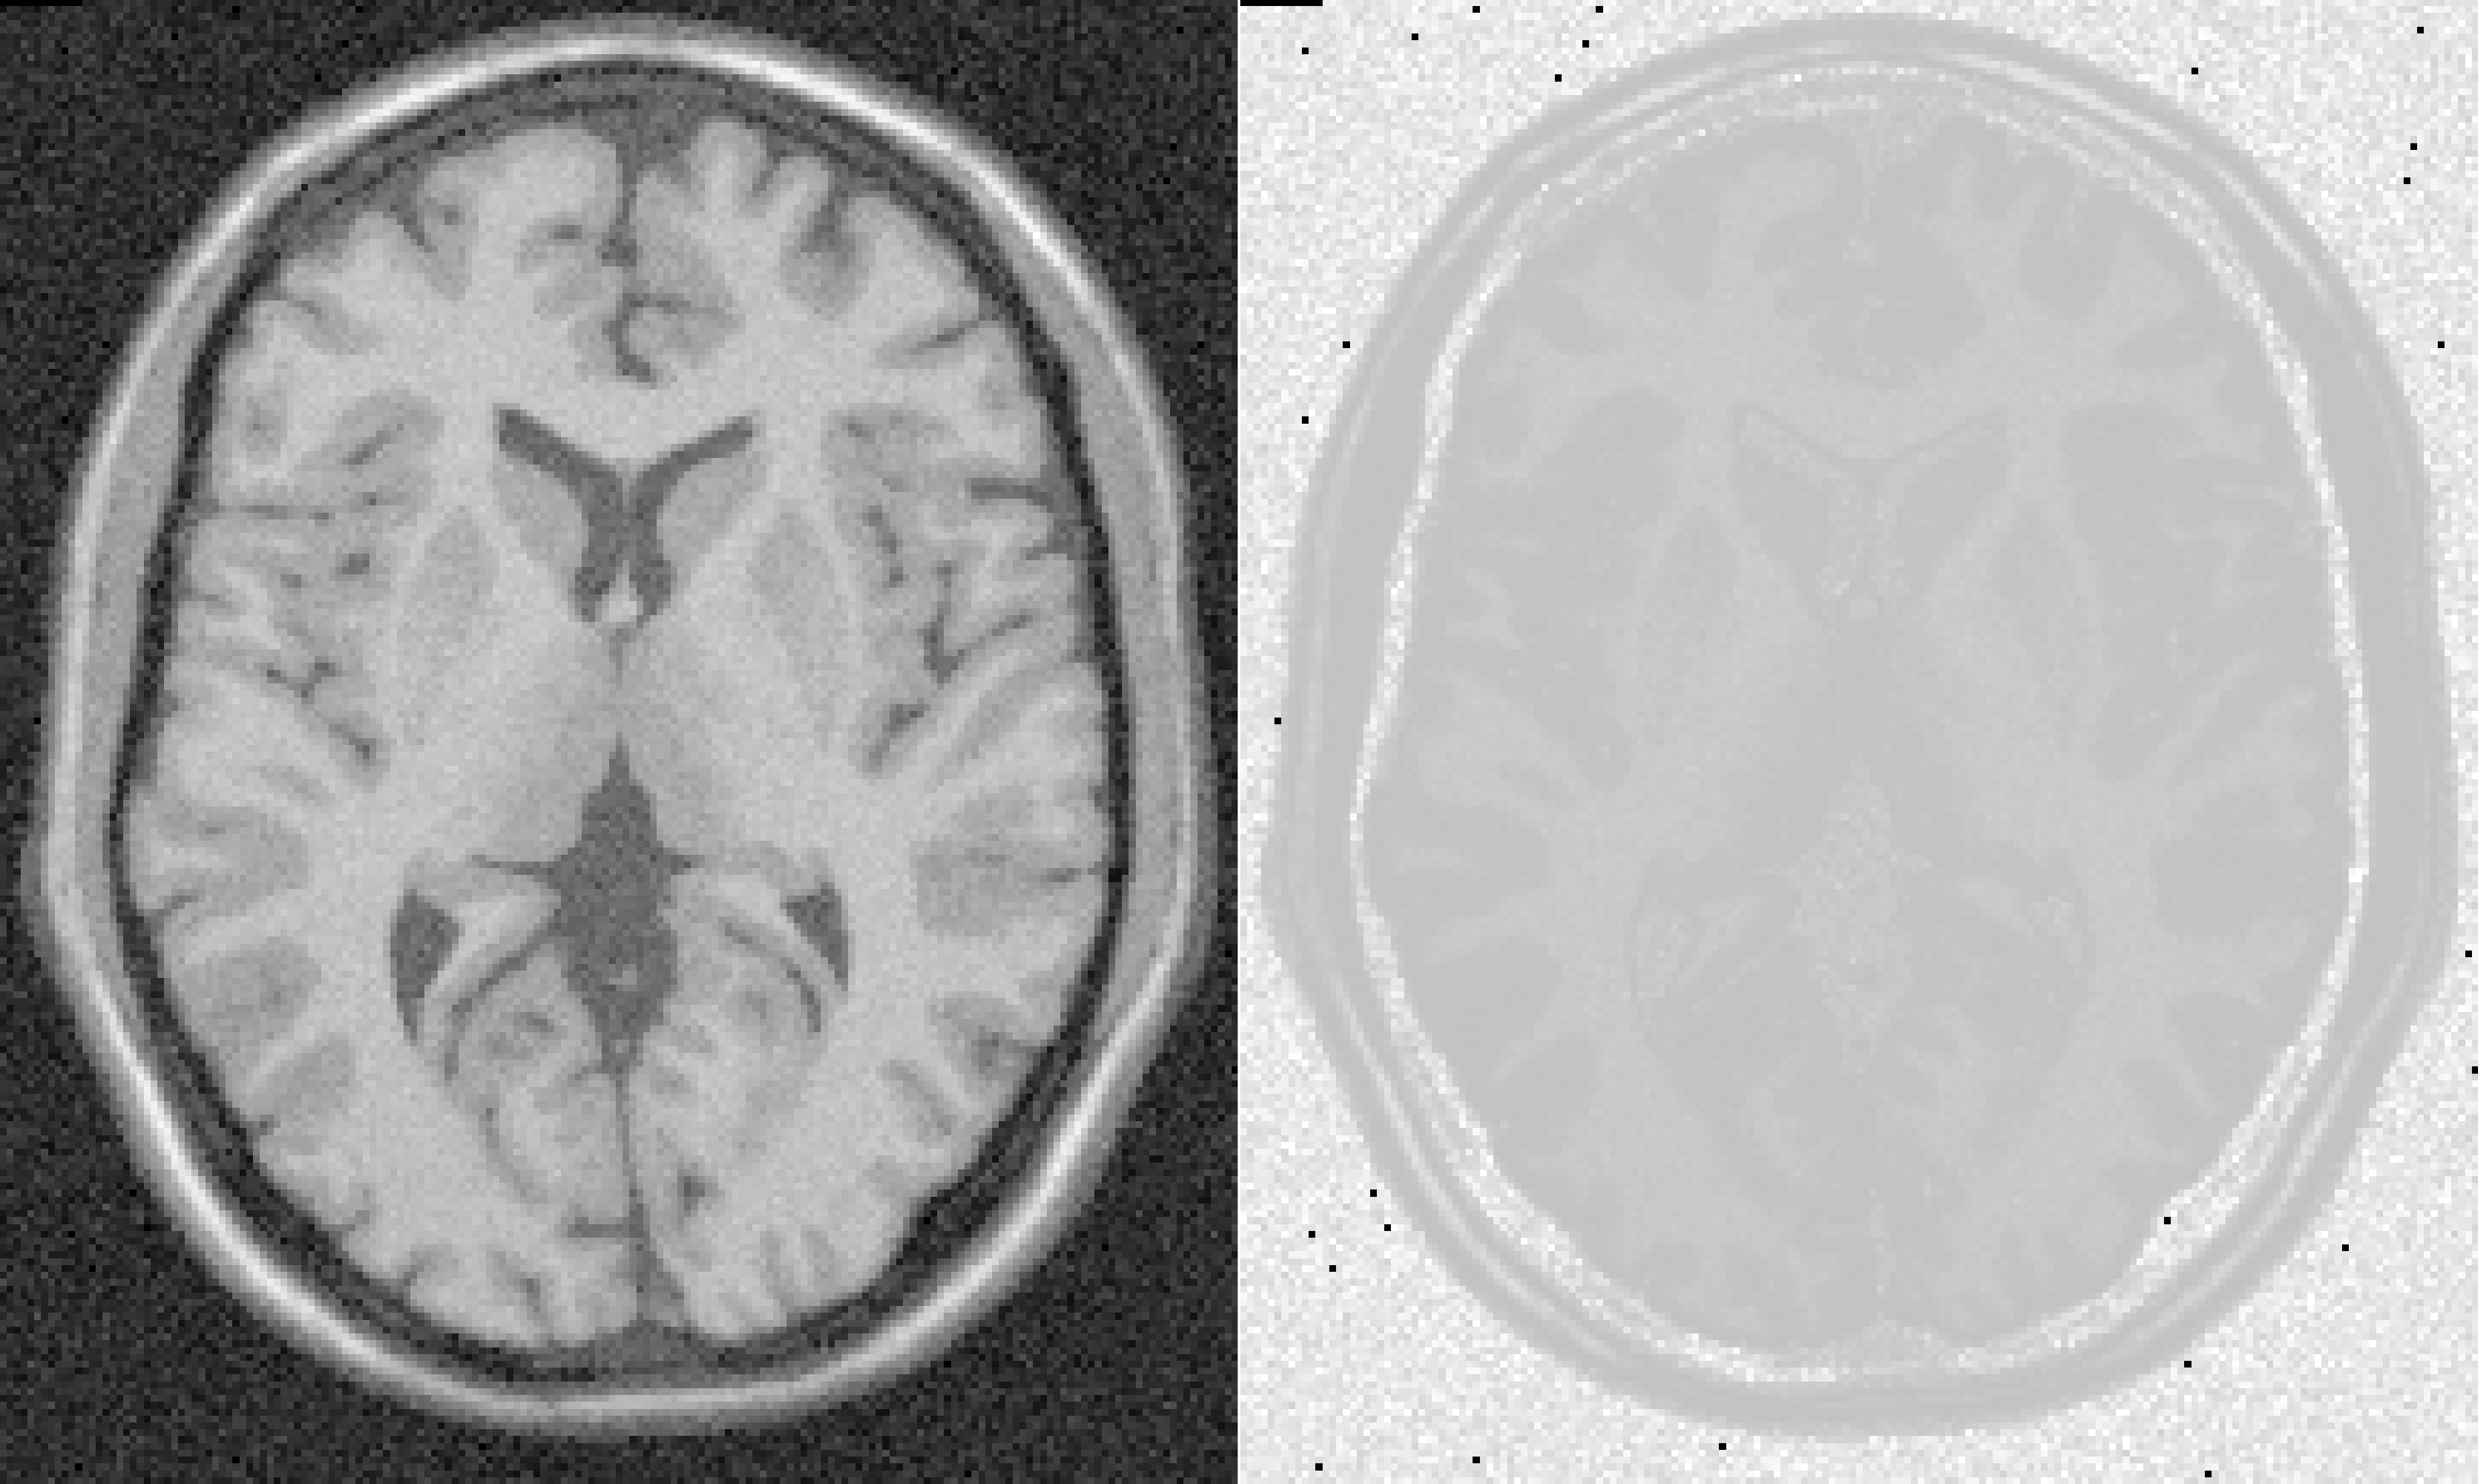
\includegraphics[width=\textwidth]{Figuras/dif_gamma=0.5.png}
            \caption{Transformación $\gamma = 0.5$.}
            \label{fig:Exptrans0.5_sustraction}
        \end{subfigure}
        \begin{subfigure}[h]{0.3\textwidth}
            \centering
            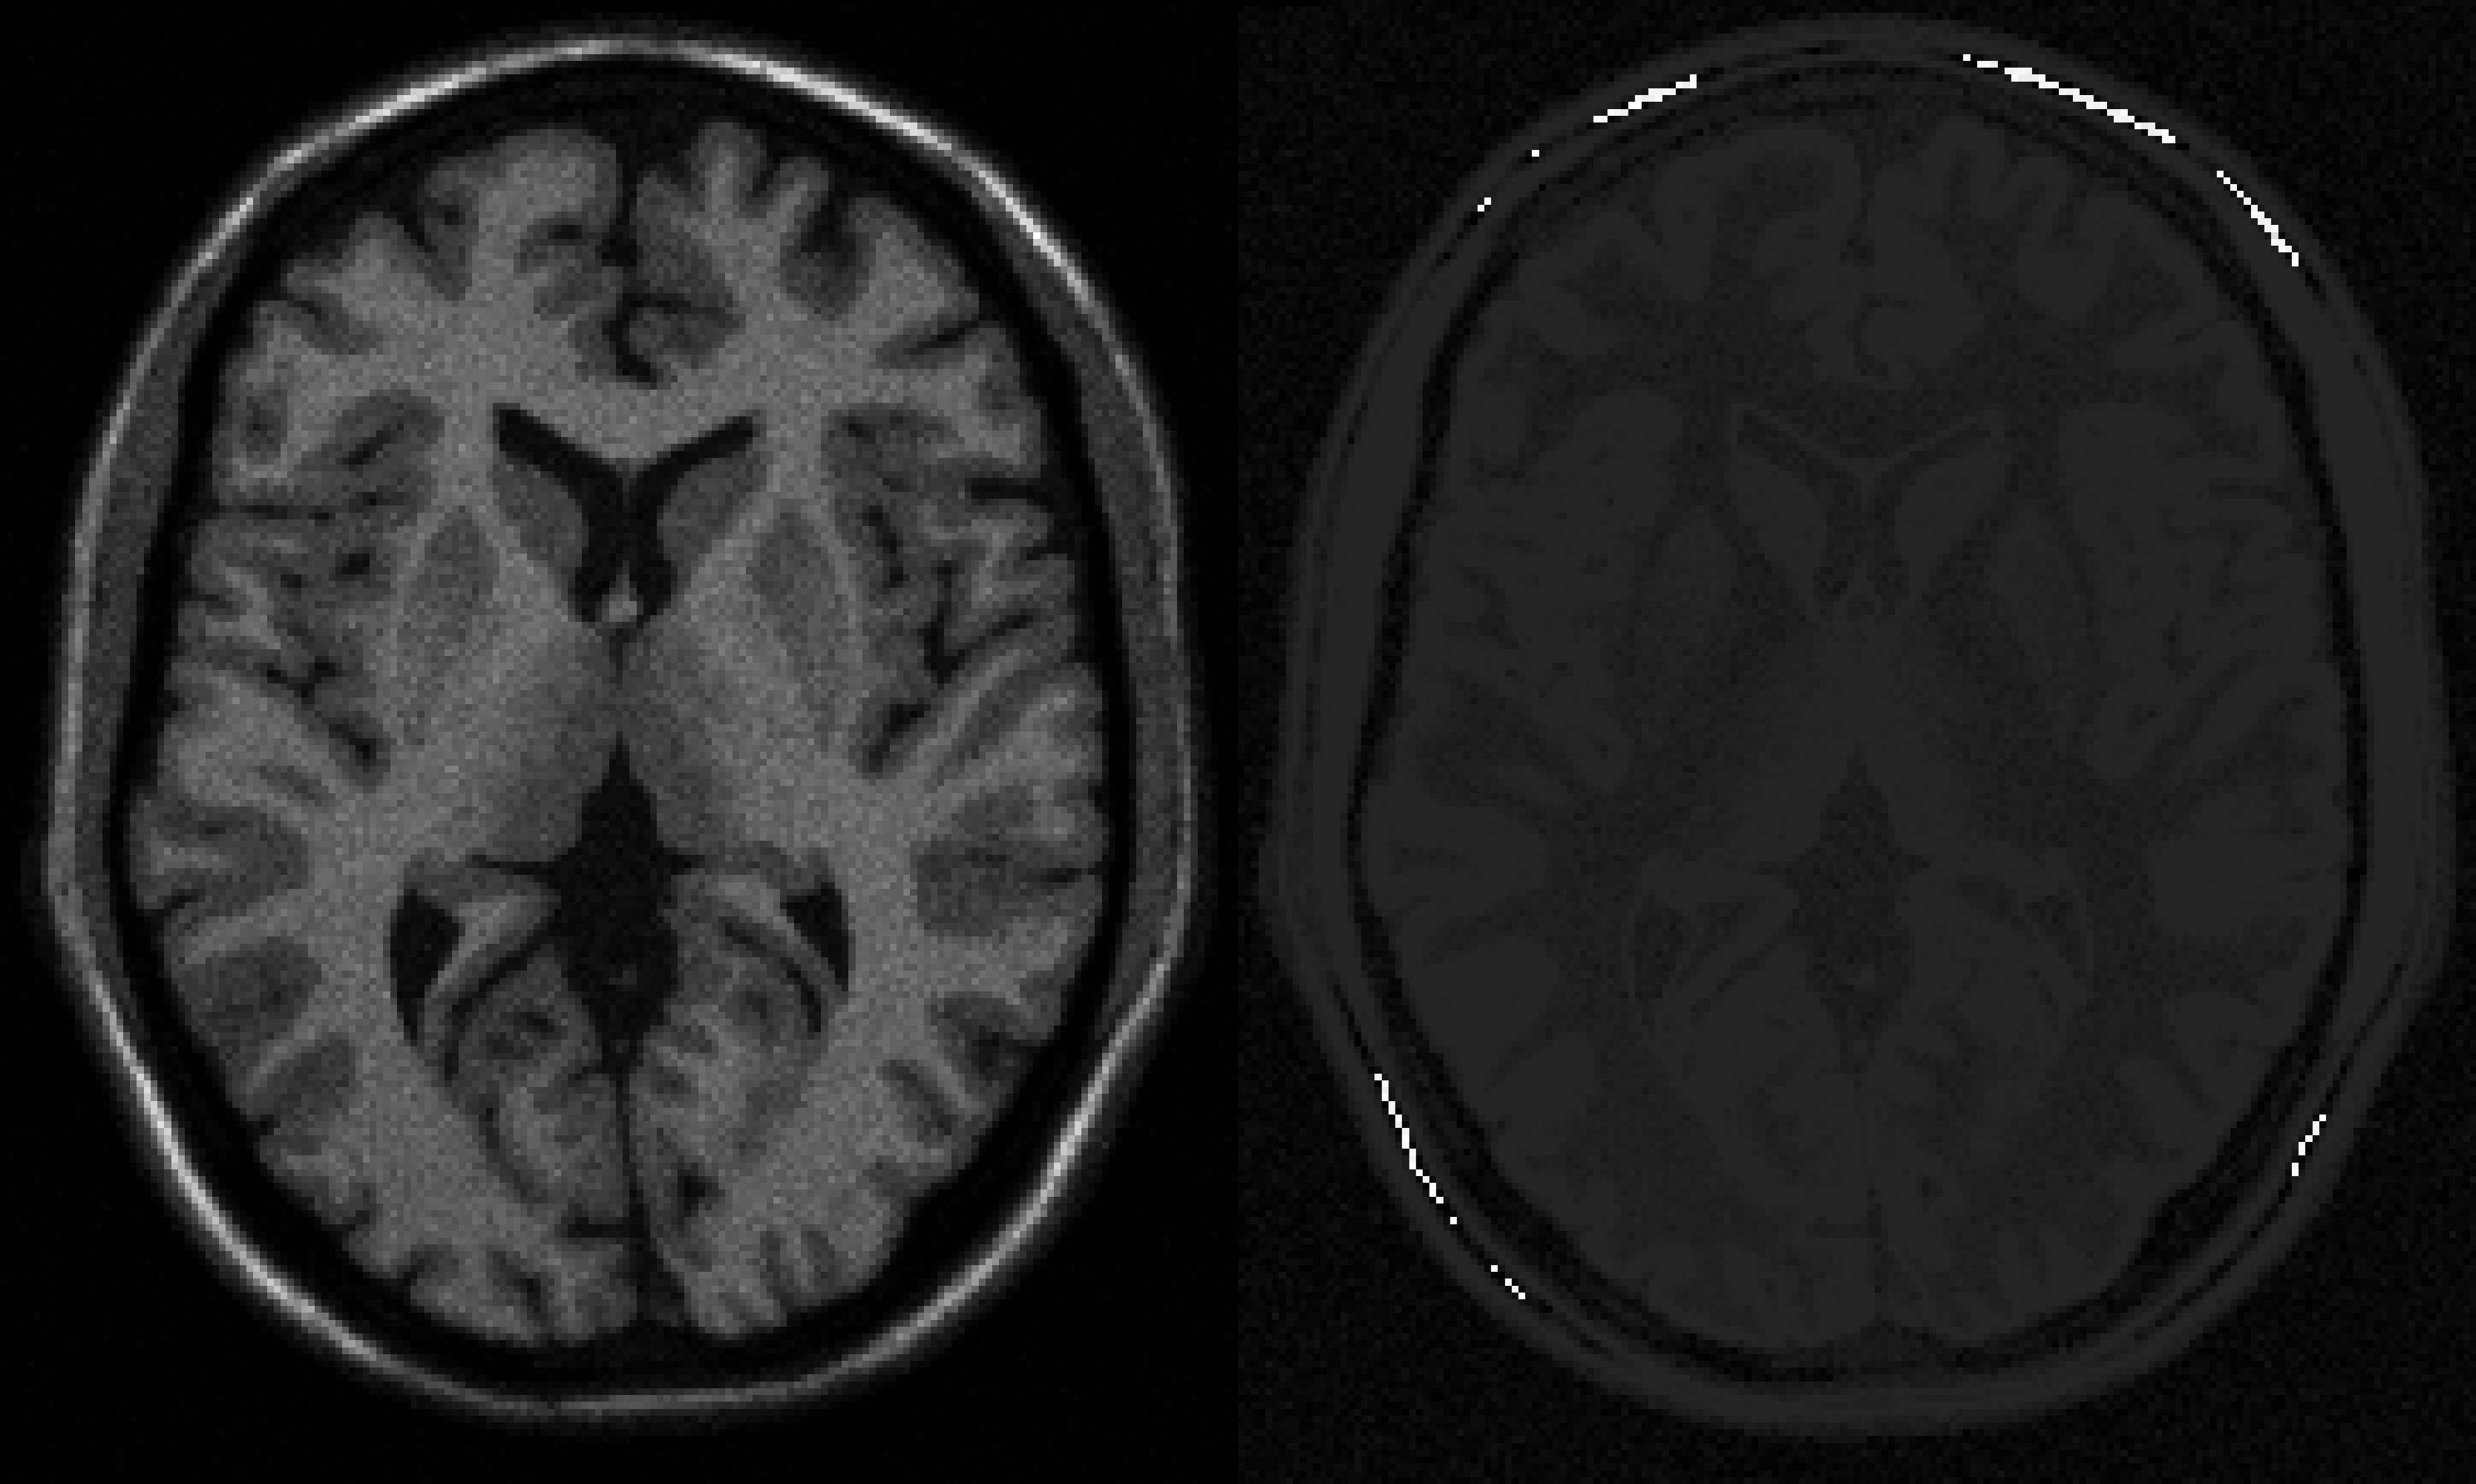
\includegraphics[width=\textwidth]{Figuras/dif_gamma=1.75.png}
            \caption{Transformación $\gamma = 1.75$.}
            \label{fig:Exptrans1.75_sustraction}
        \end{subfigure}
        \caption{Diferencia entre la la imagen A original y las transformaciones aplicadas.}
\end{figure}

\section{Interpolación \label{sec:ej3}}

\vspace{0.3cm}

Se tomó la $\verb|ImagenC.pgm|$ de tamaño $128\times128$ pixels$^2$ y se interpoló utilizando el método de vecinos más cercanos y bilineal implementados en $\verb|ImagenA.pgm|$ para obtener imágenes de $32\times32$, $64\times64$, $256\times256$ y $1024\times1024$ pixels$^2$. La implementación de ambas técnicas se realizó en python. Los resultados se muestran en la Fig. \ref{fig:Interpolate}. Se observa que la interpolación bilineal es más suave en la transición de la escala de grises que la interpolación por vecinos más cercanos.

\begin{figure}[H]
    \centering
        \begin{subfigure}[h]{0.24\textwidth}
            \centering
            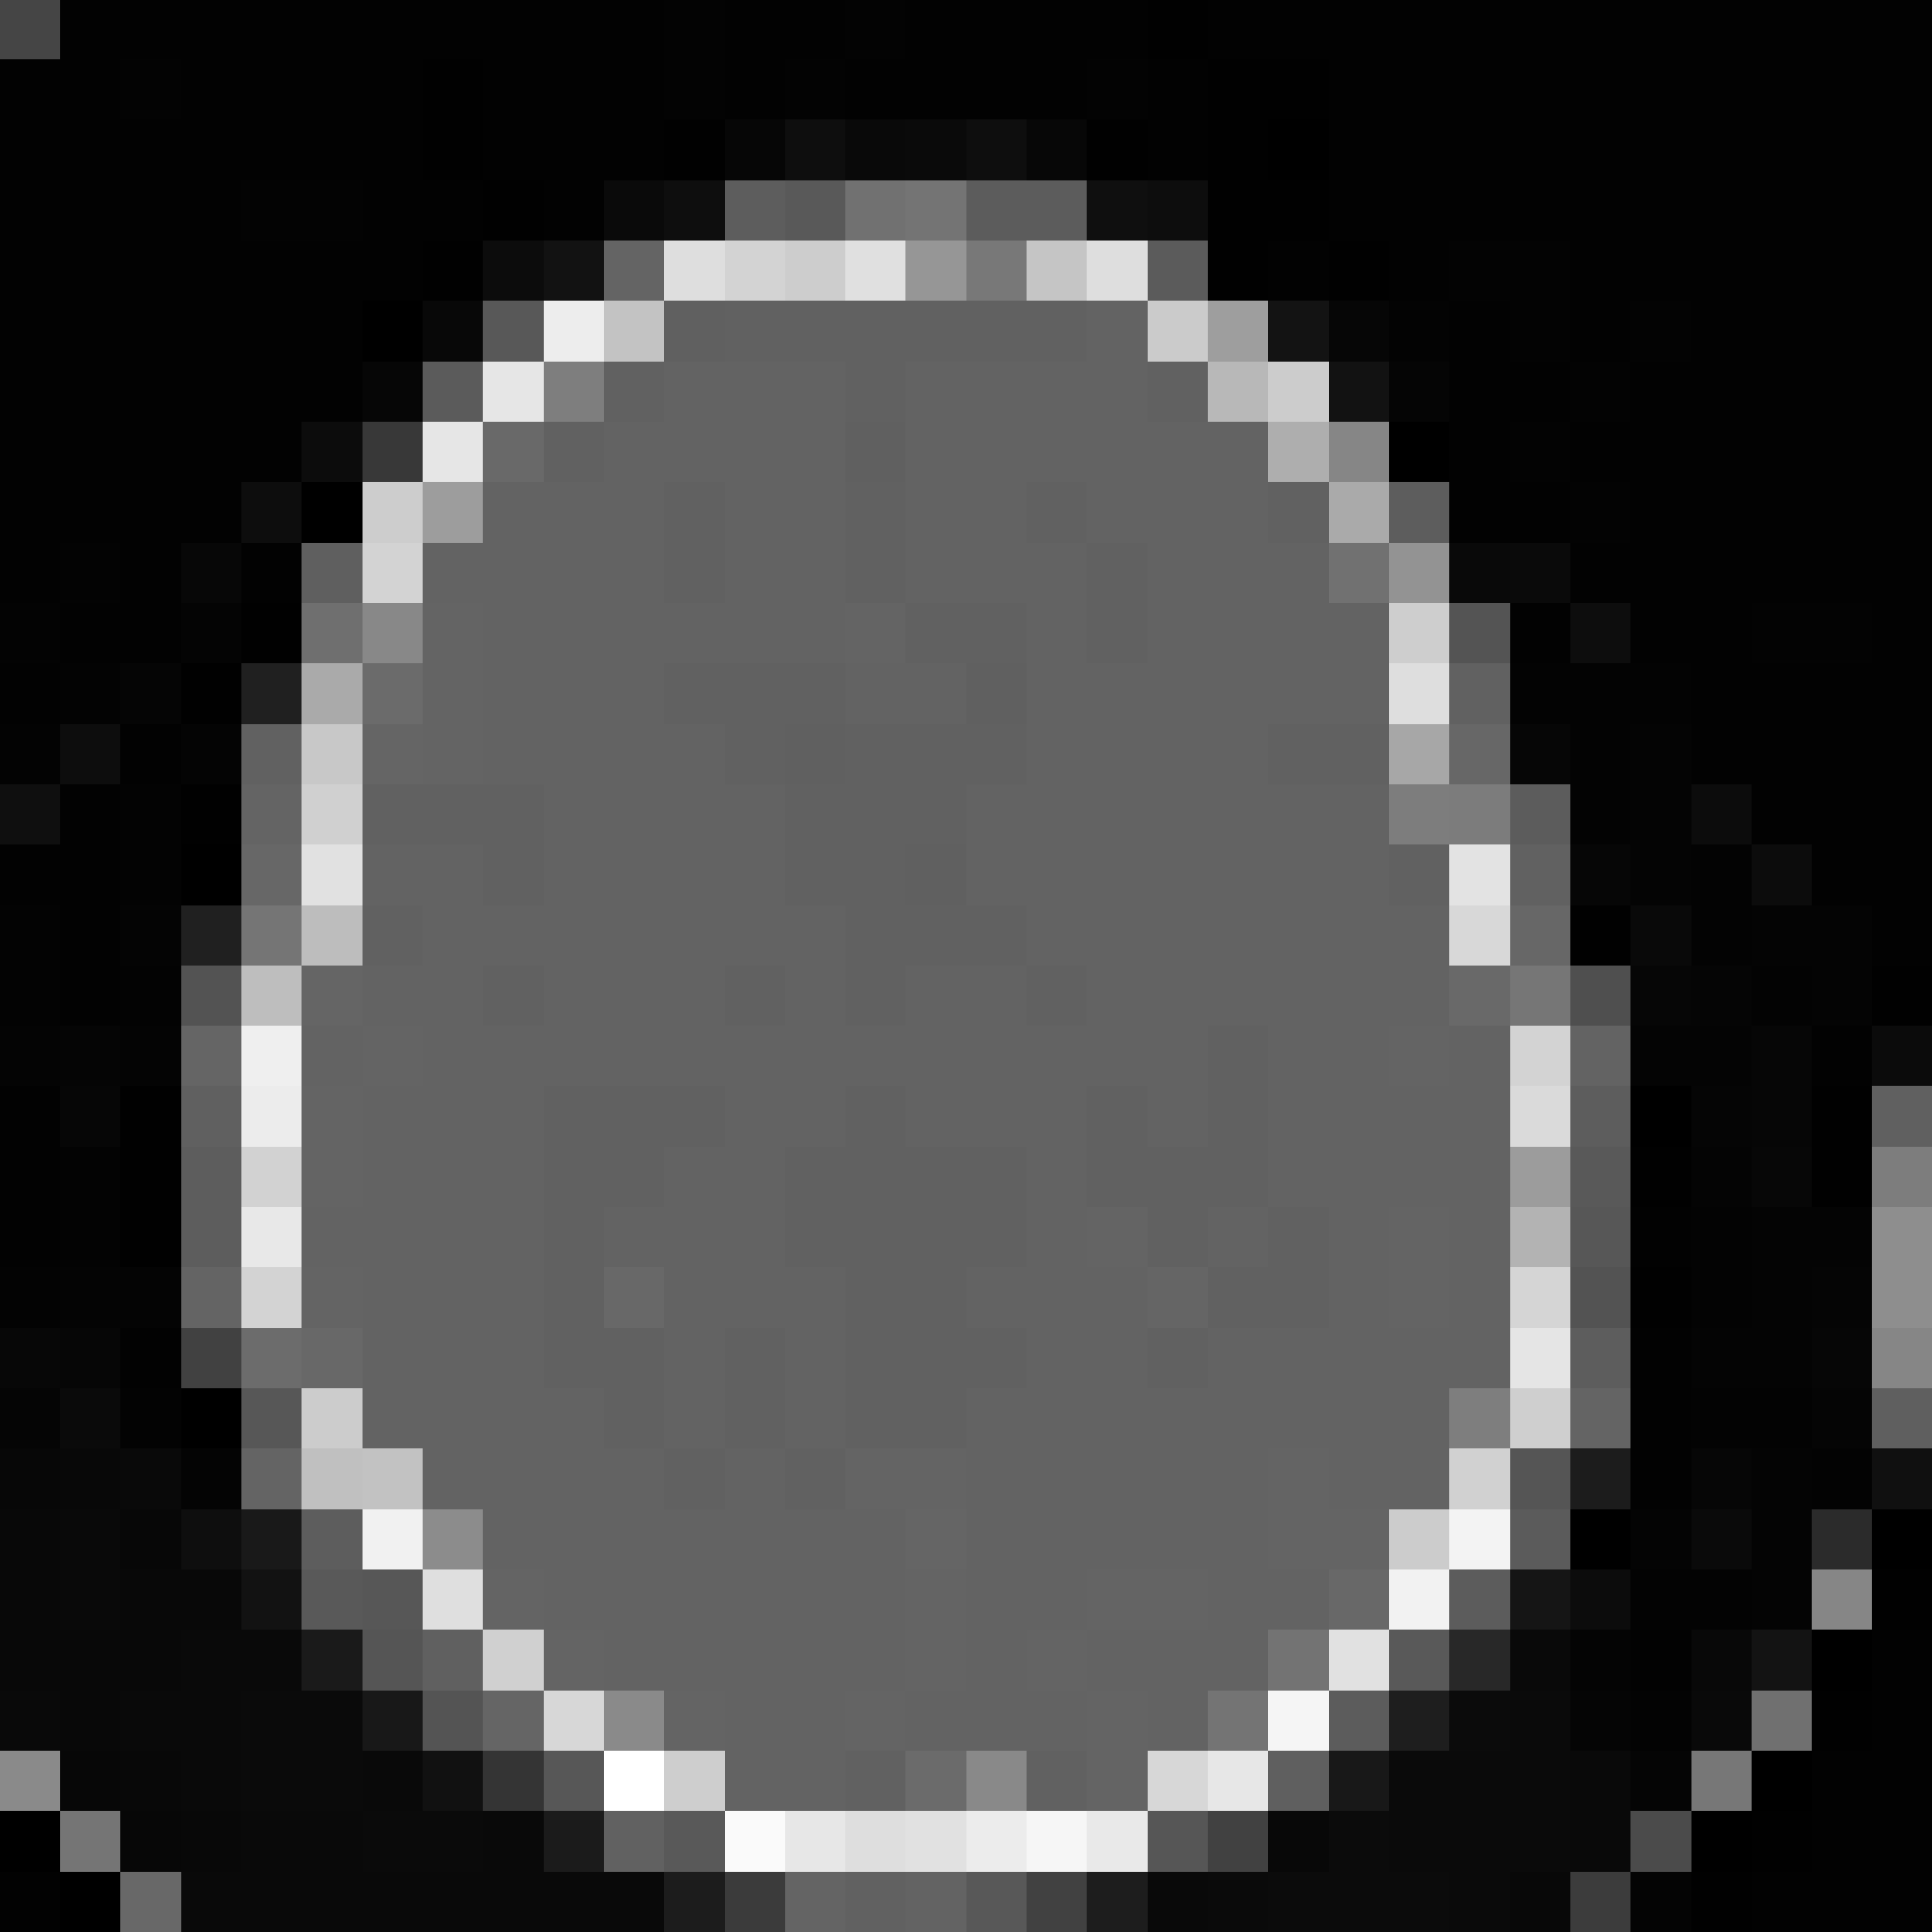
\includegraphics[width=\textwidth]{Figuras/Interpolate_nn_f=0.25.png} 
        \end{subfigure}
        \begin{subfigure}[h]{0.24\textwidth}
            \centering
            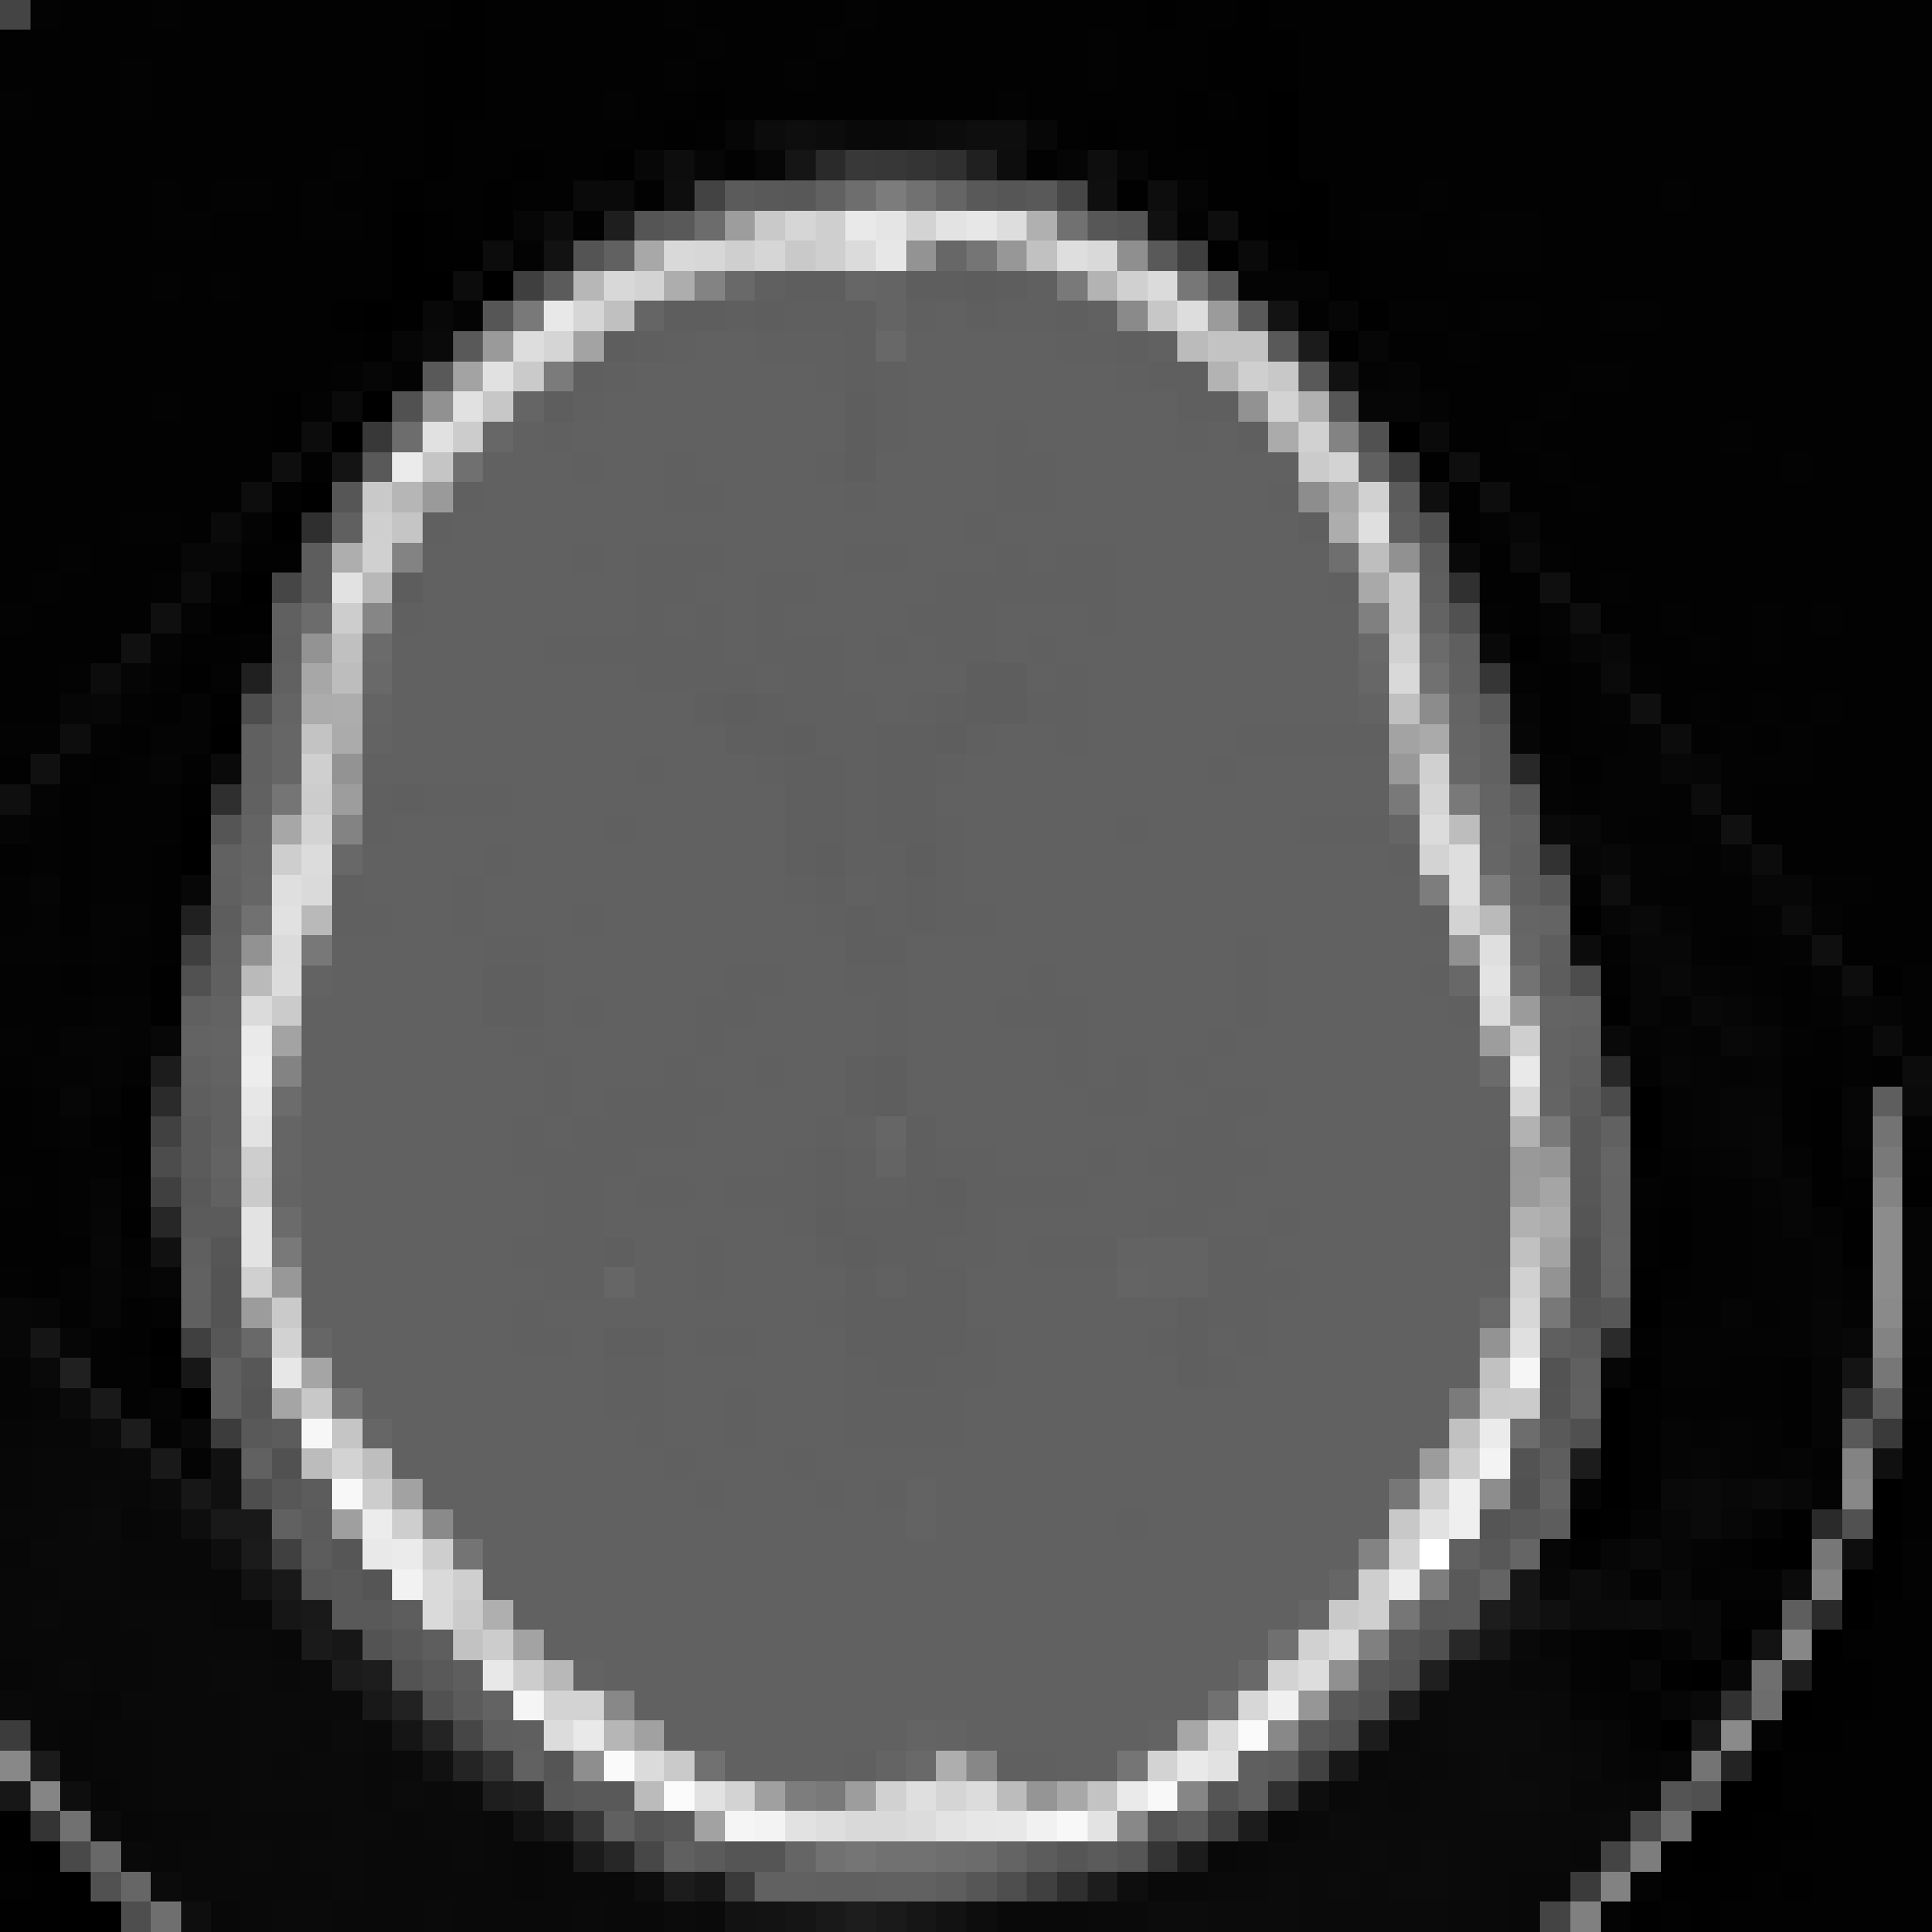
\includegraphics[width=\textwidth]{Figuras/Interpolate_nn_f=0.5.png}
        \end{subfigure}
        \begin{subfigure}[h]{0.24\textwidth}
            \centering
            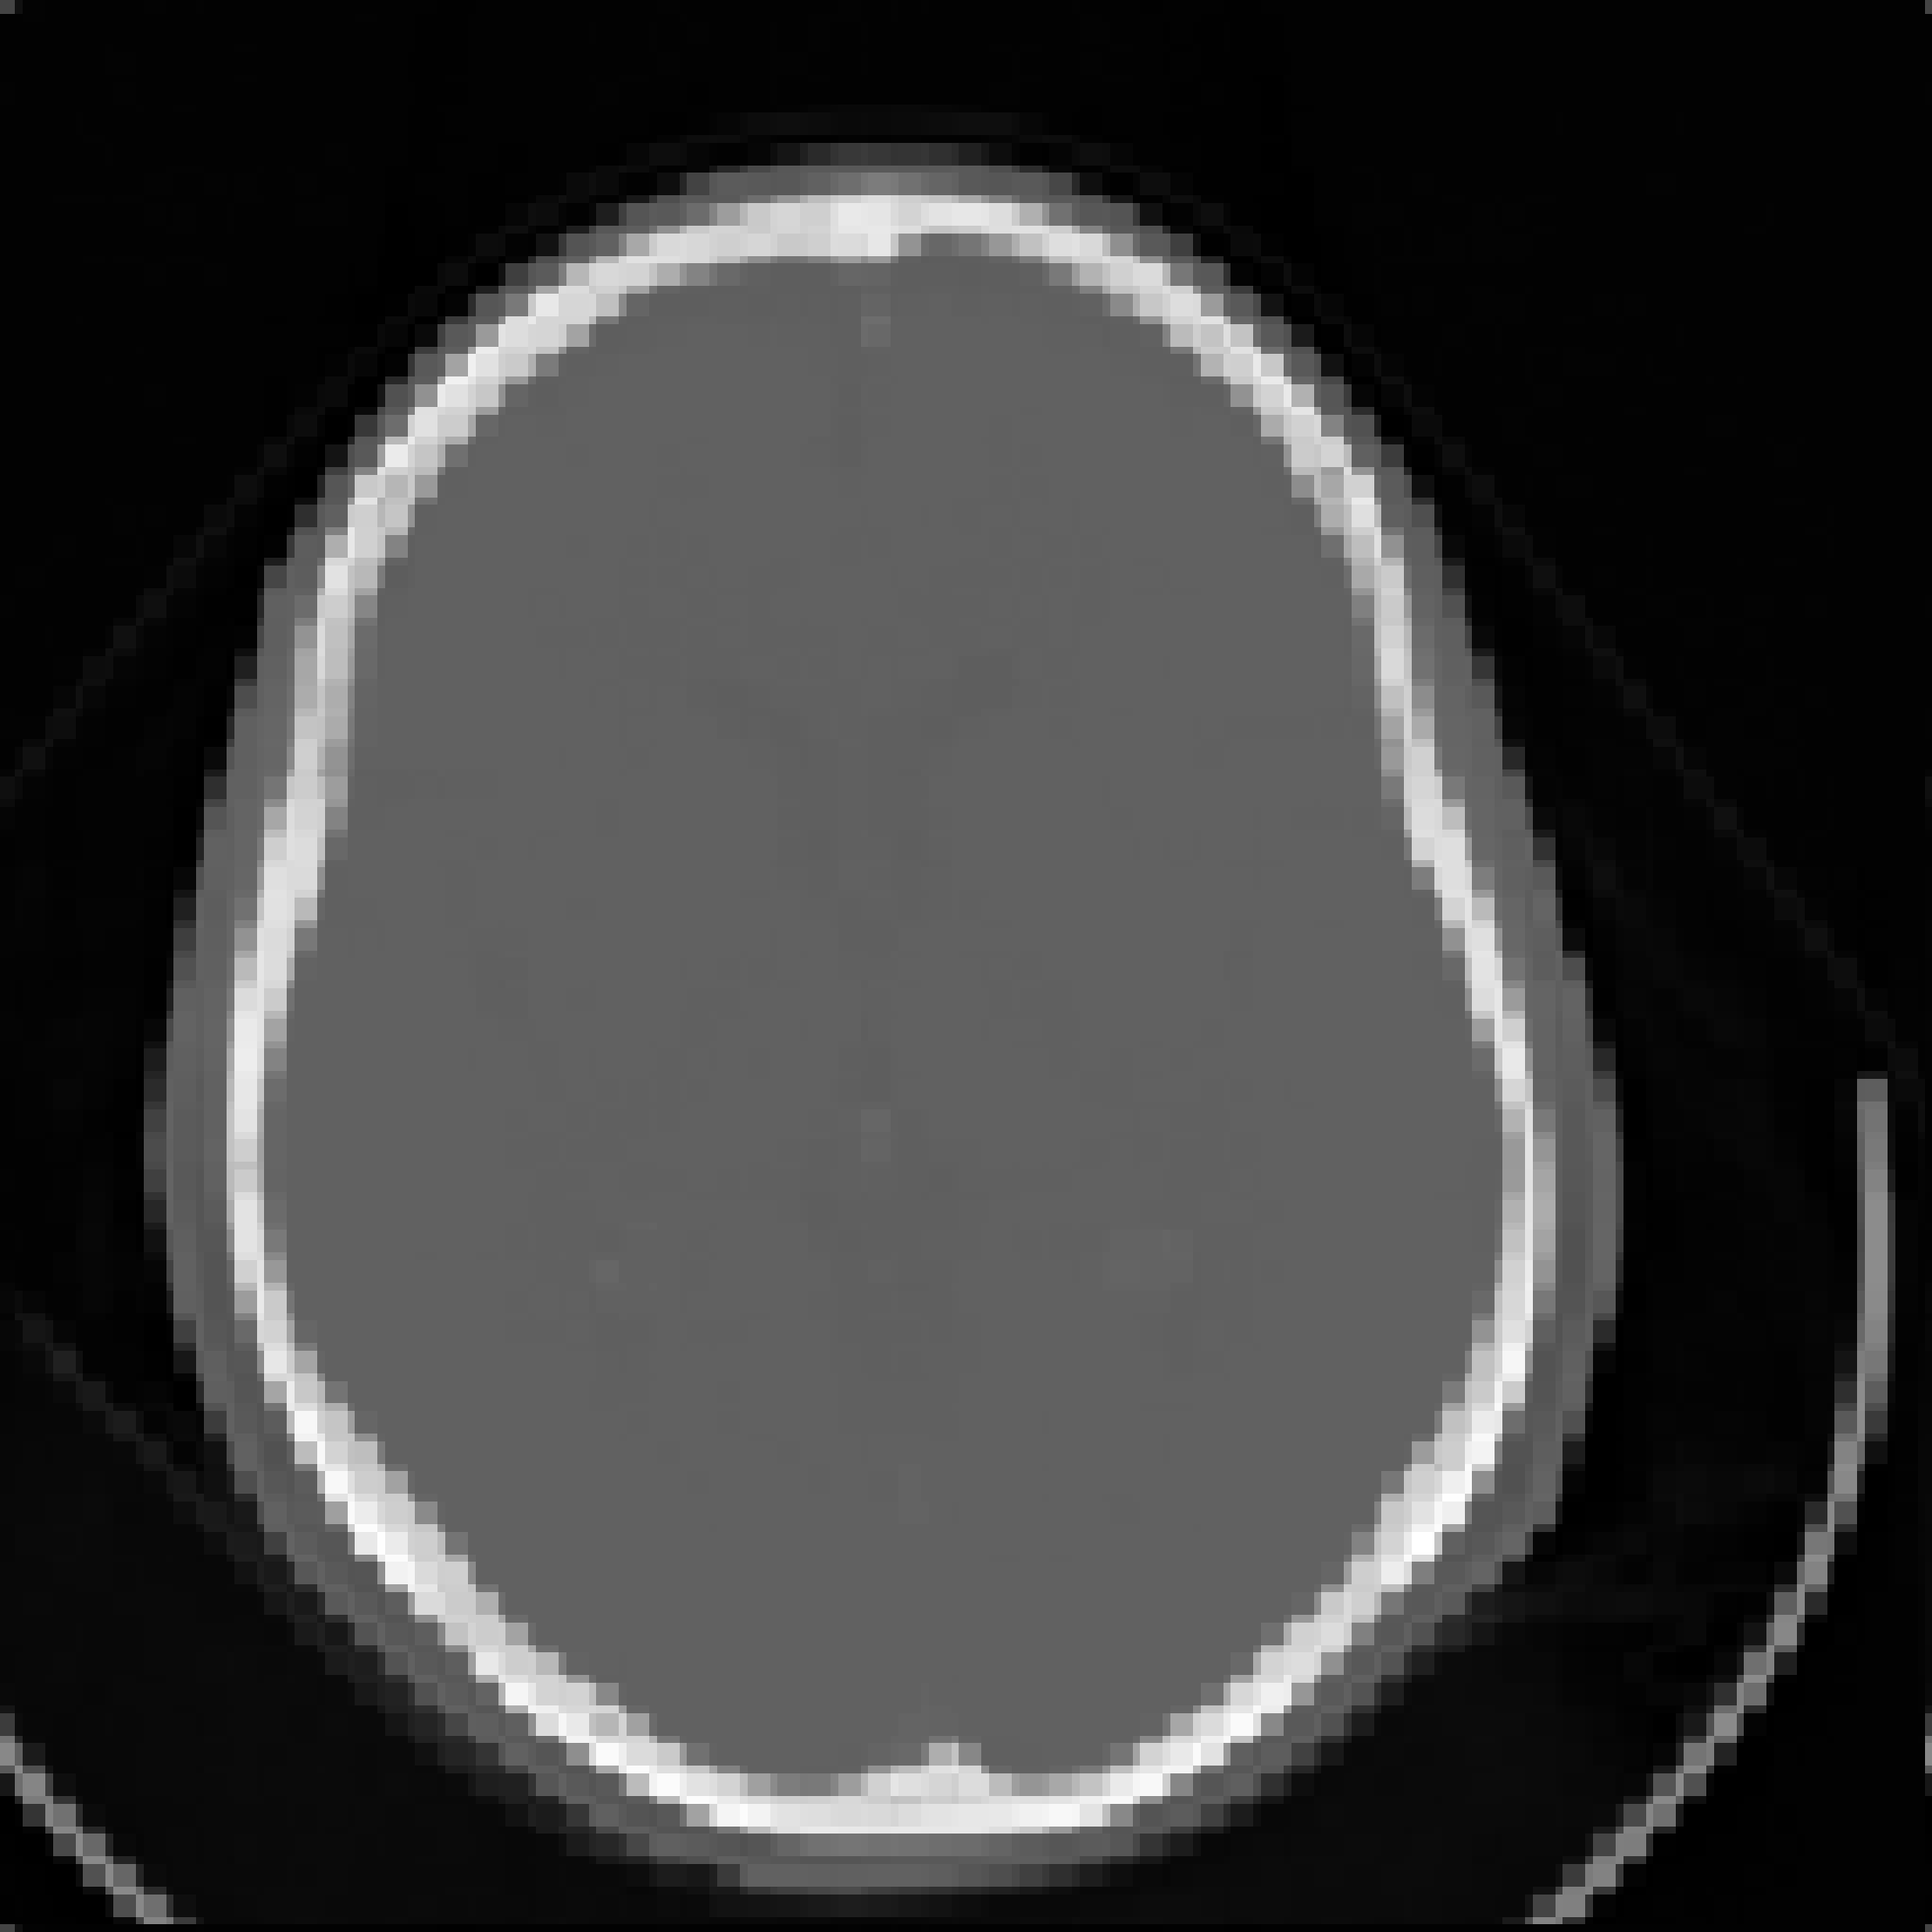
\includegraphics[width=\textwidth]{Figuras/Interpolate_nn_f=2.png}
        \end{subfigure}
        \begin{subfigure}[h]{0.24\textwidth}
            \centering
            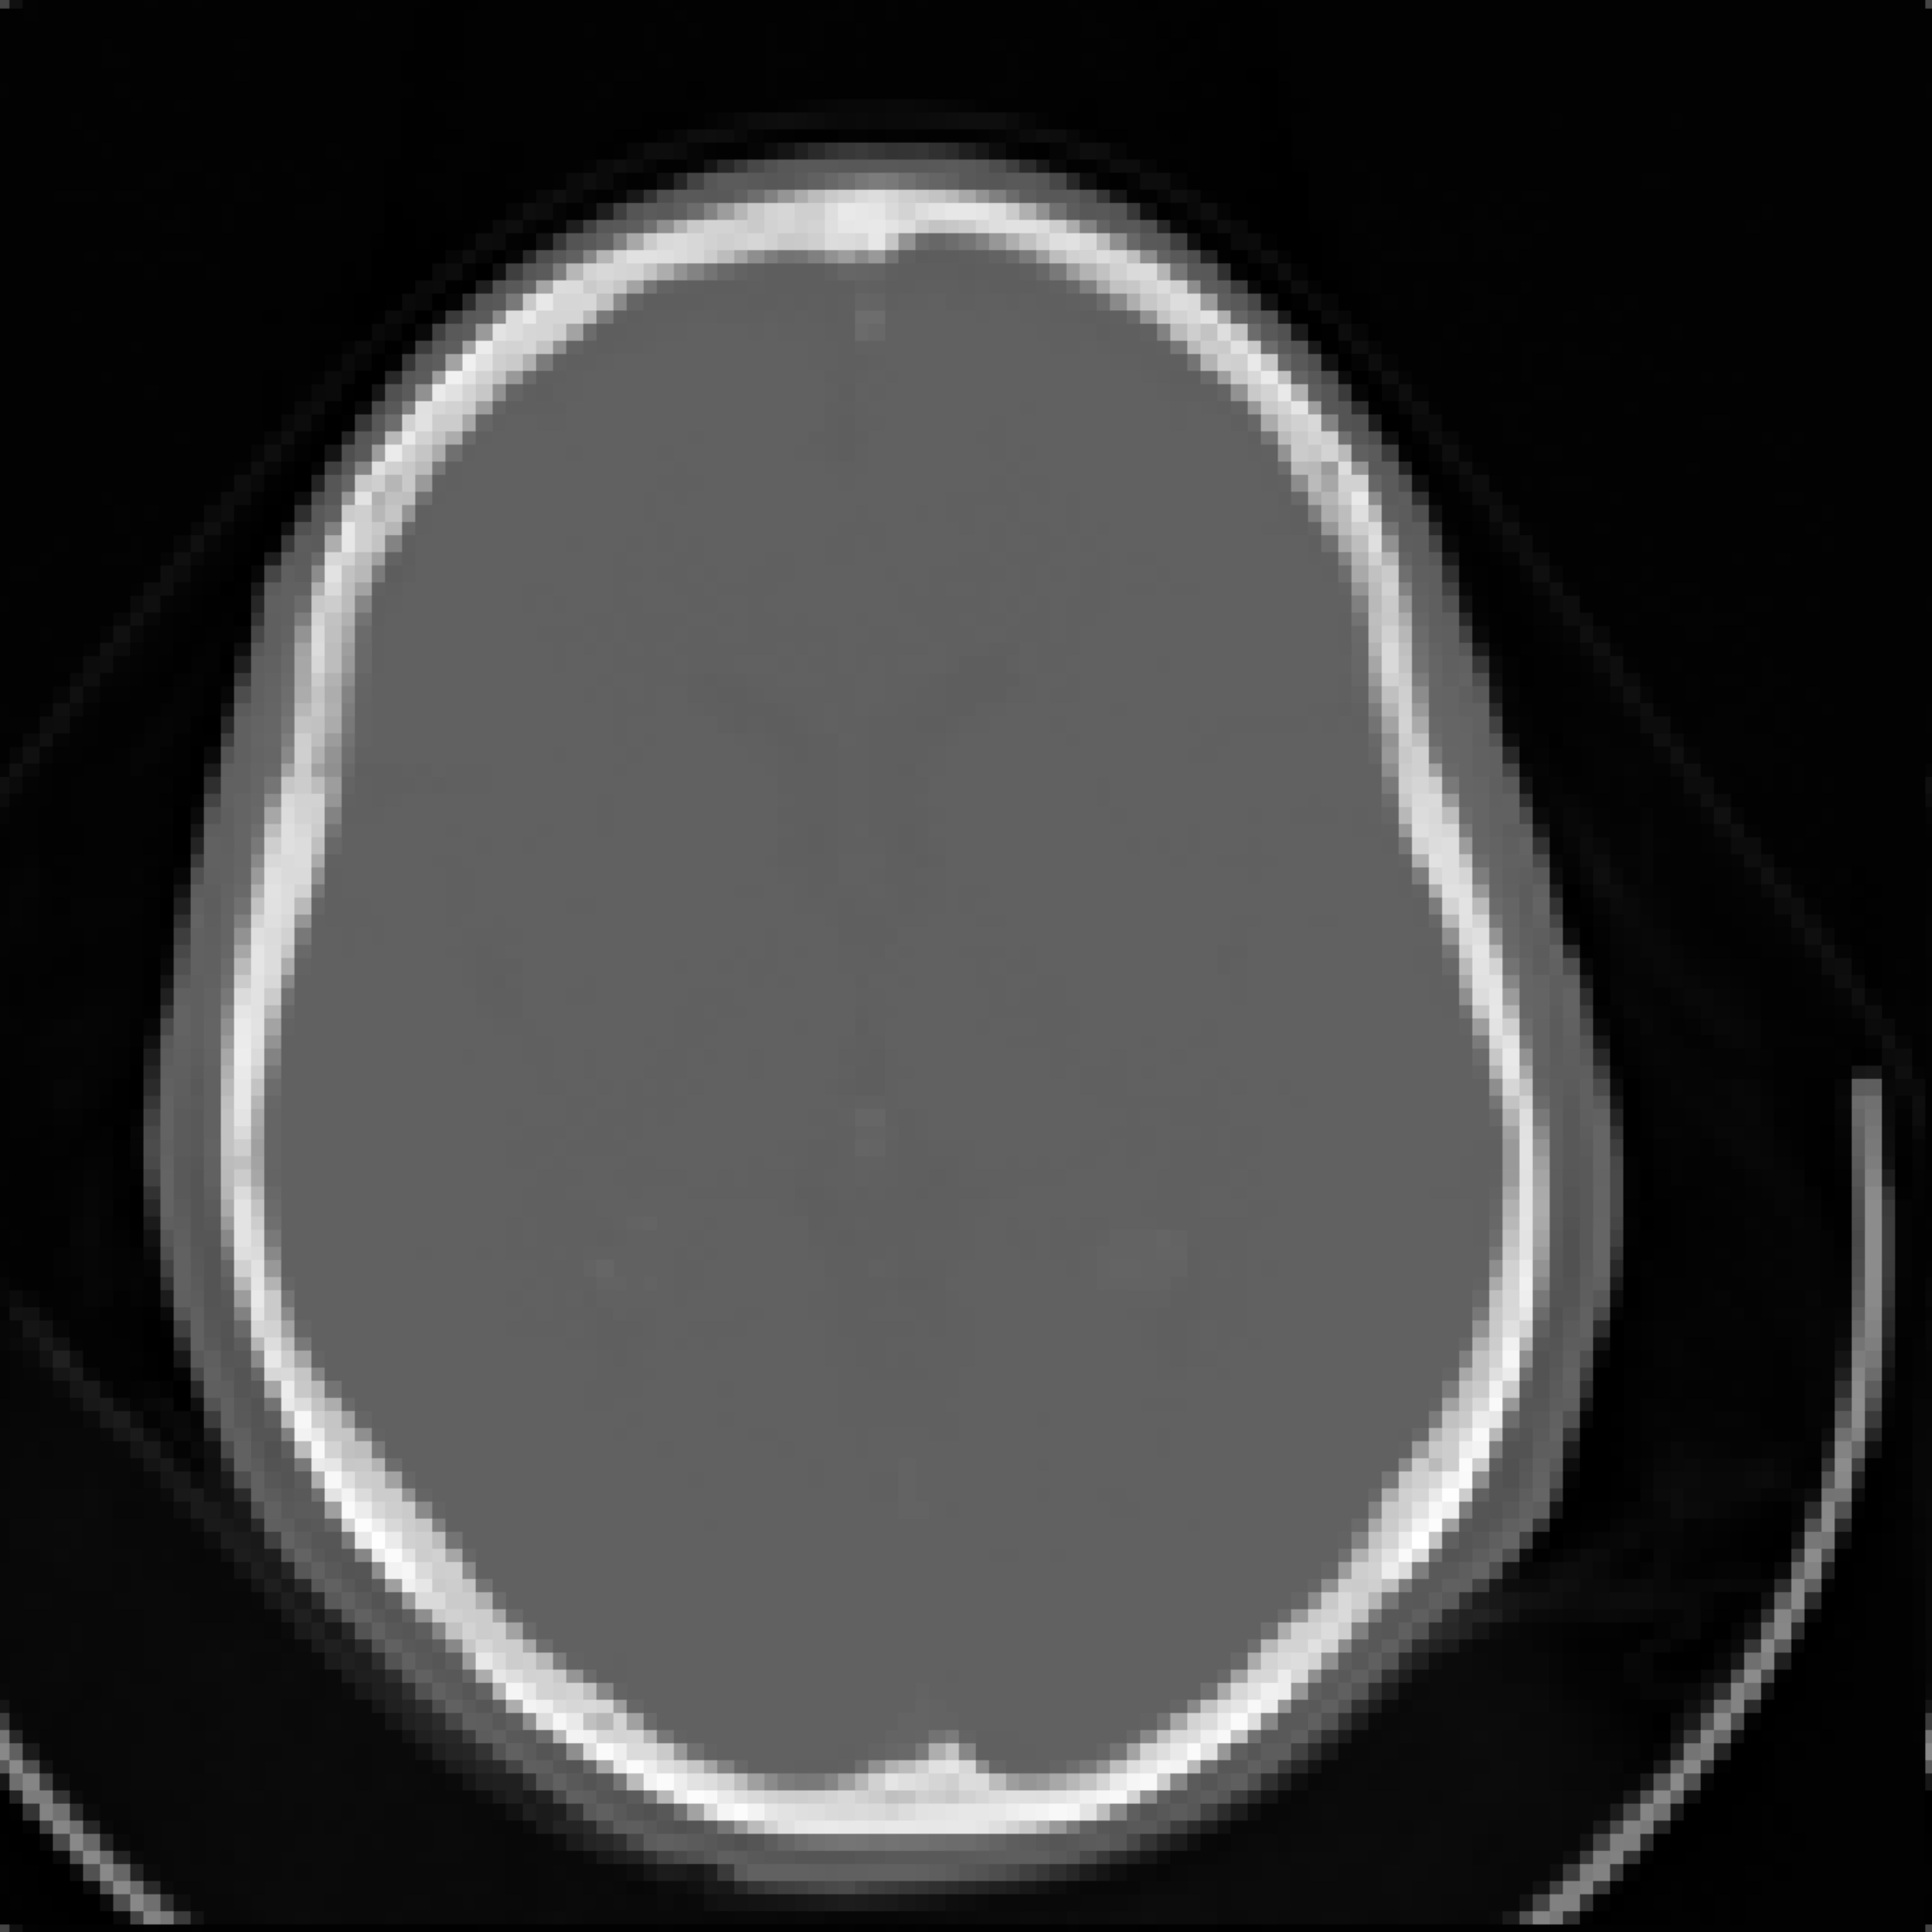
\includegraphics[width=\textwidth]{Figuras/Interpolate_nn_f=8.png}
        \end{subfigure}
         \begin{subfigure}[h]{0.24\textwidth}
            \centering
            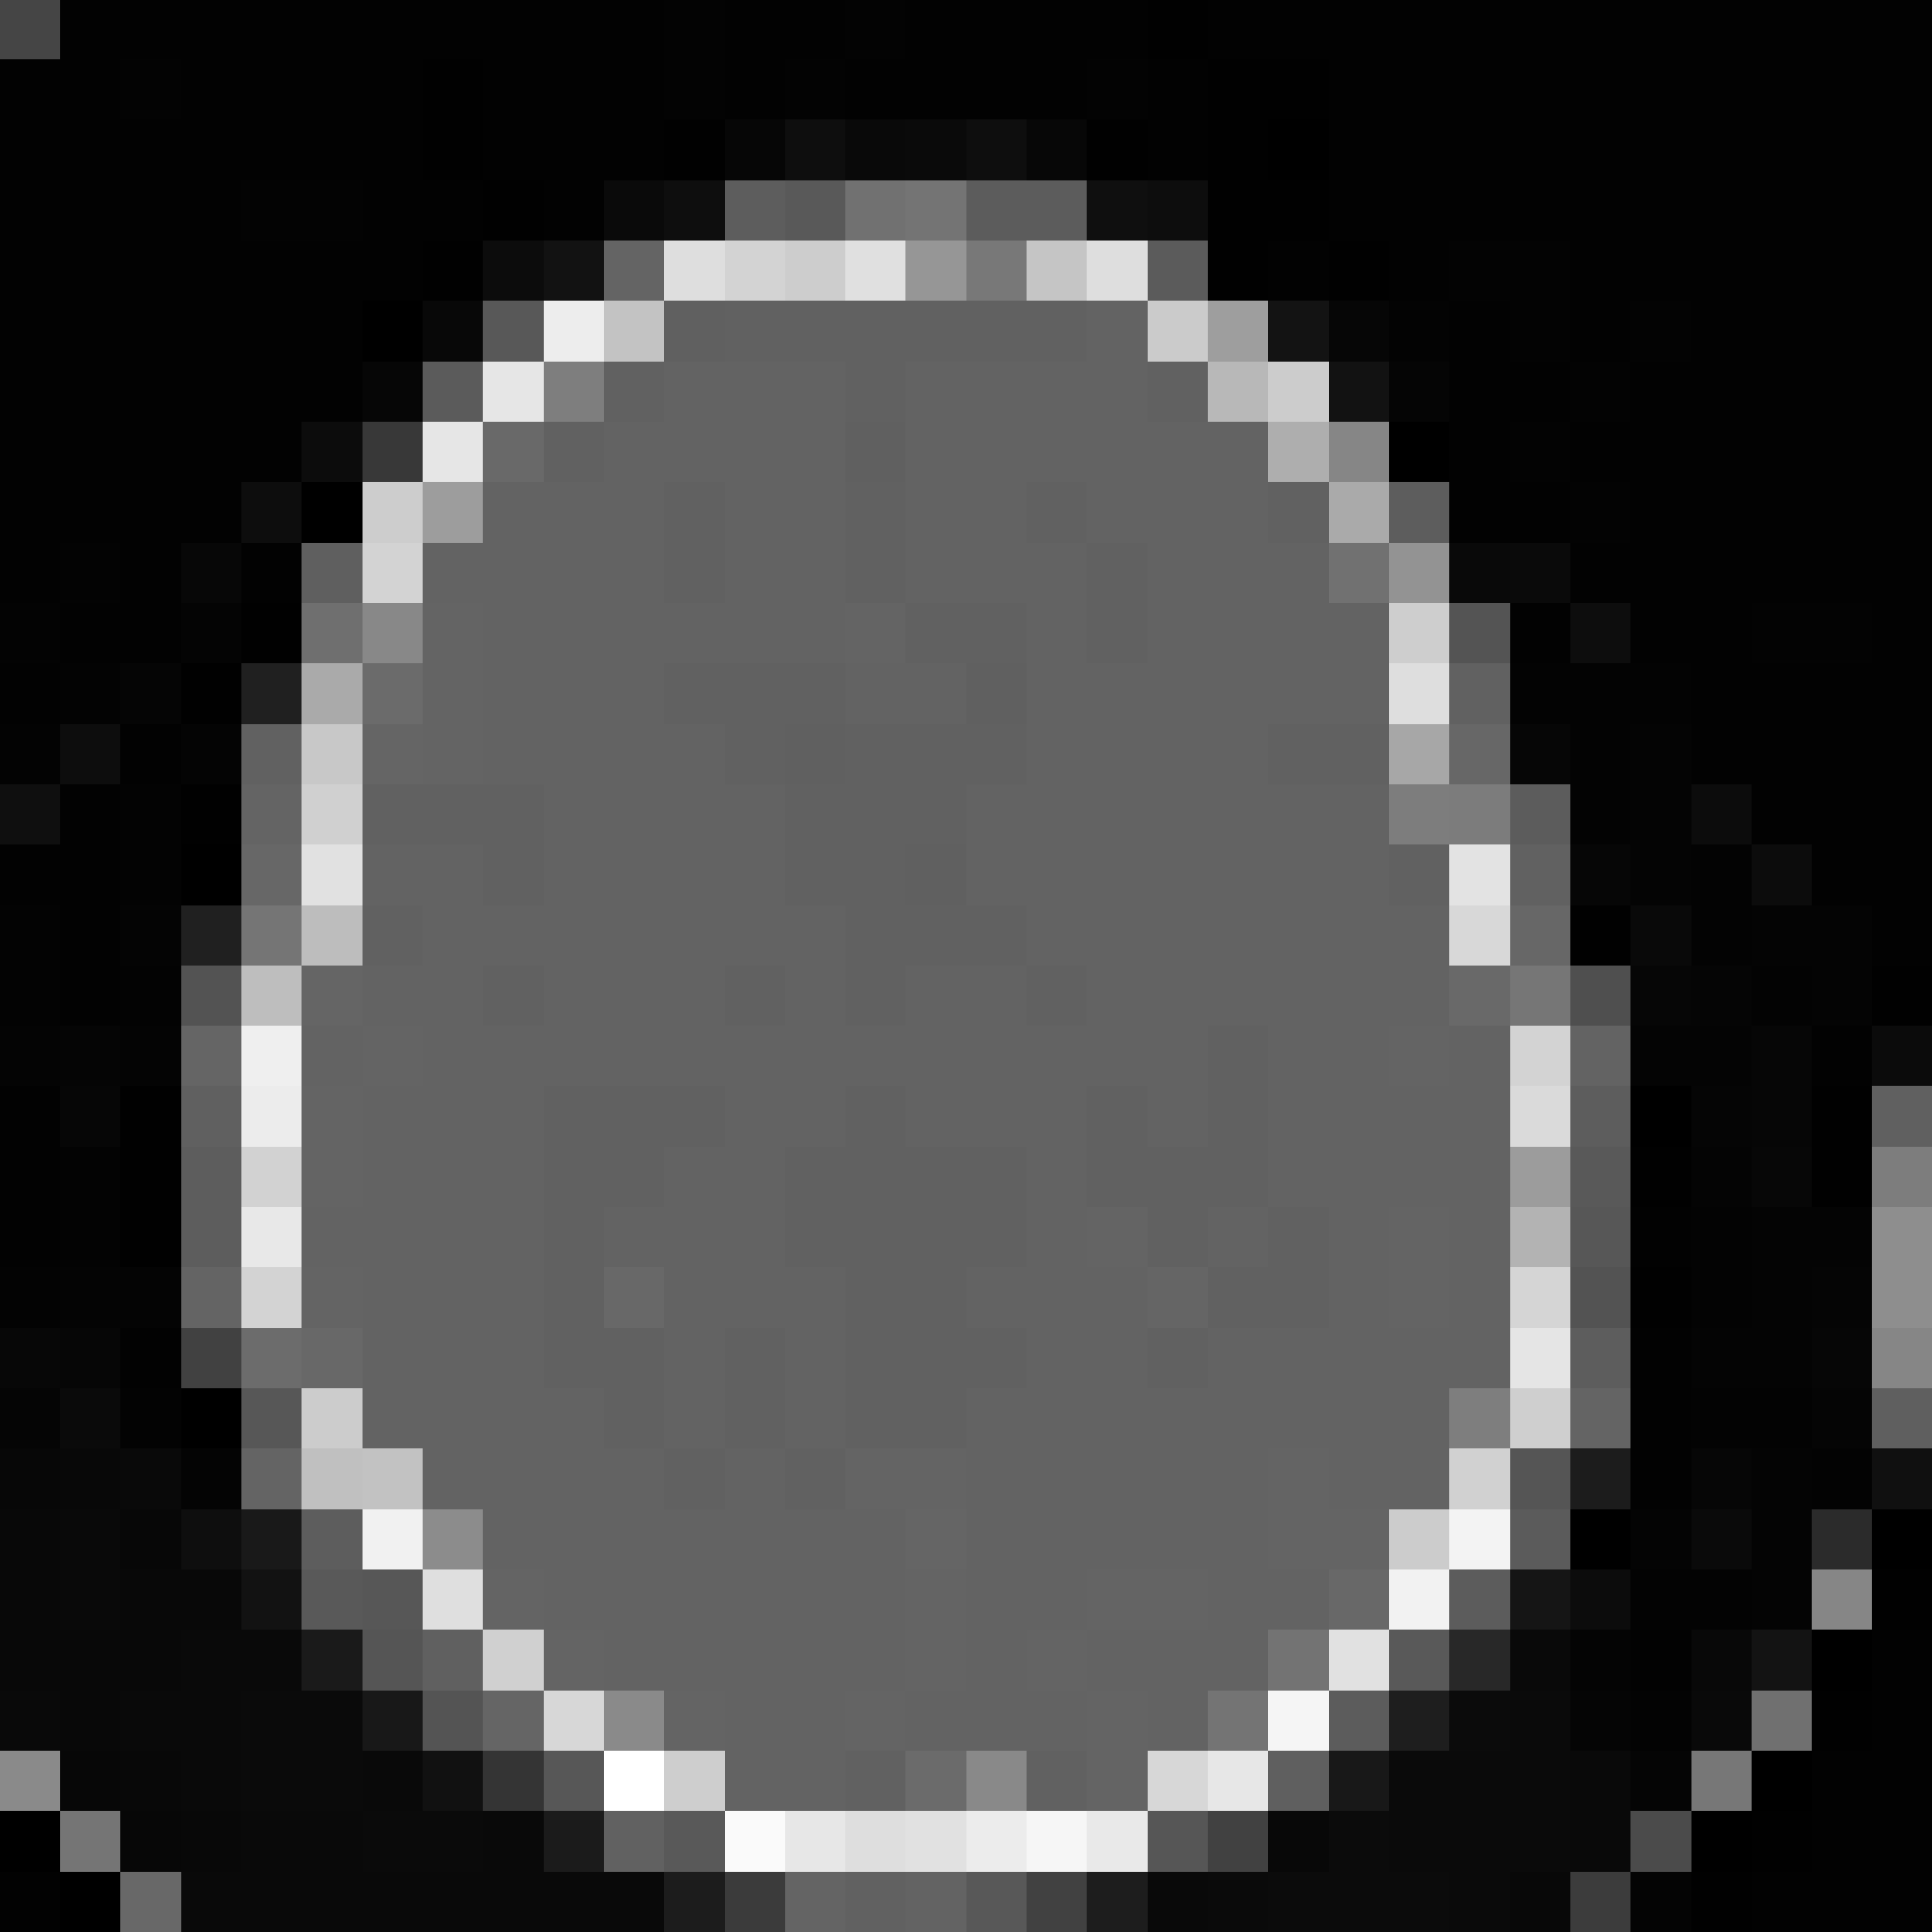
\includegraphics[width=\textwidth]{Figuras/Interpolate_bilinear_f=0.25.png}
            \caption{$32\times32$} 
         \end{subfigure}
         \begin{subfigure}[h]{0.24\textwidth}
            \centering
            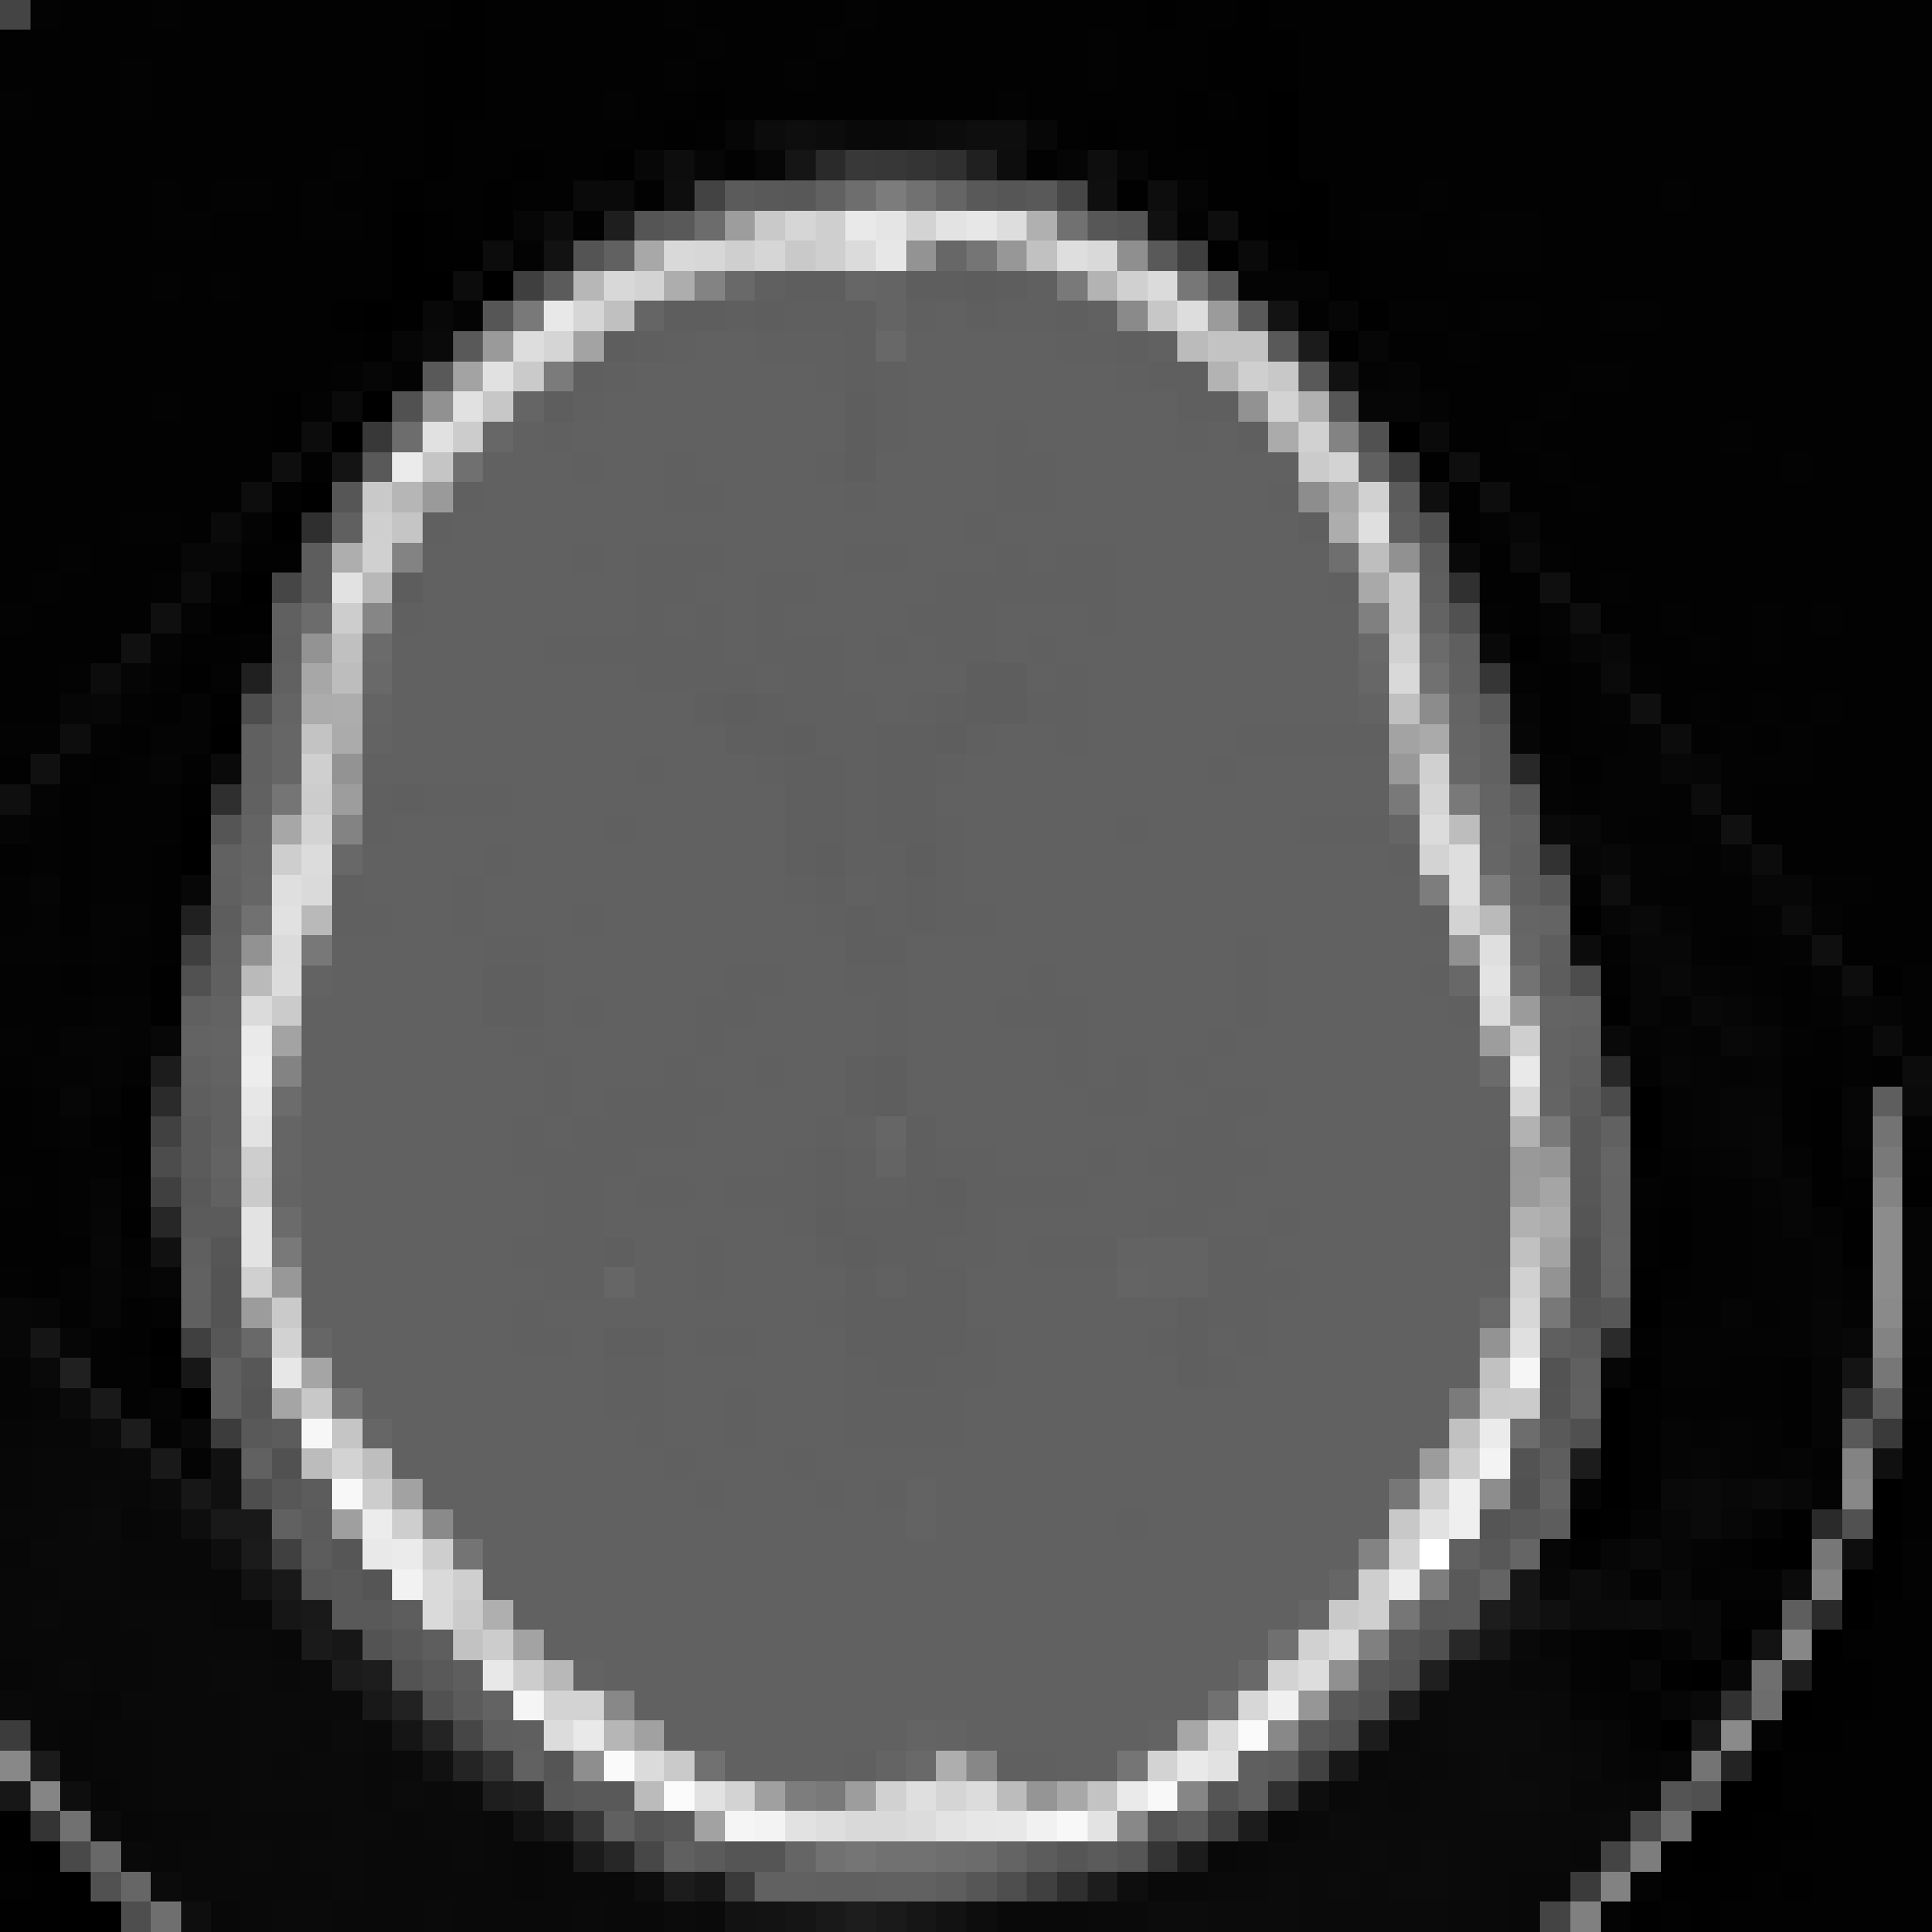
\includegraphics[width=\textwidth]{Figuras/Interpolate_bilinear_f=0.5.png}
            \caption{$64\times64$} 
         \end{subfigure}
         \begin{subfigure}[h]{0.24\textwidth}
            \centering
            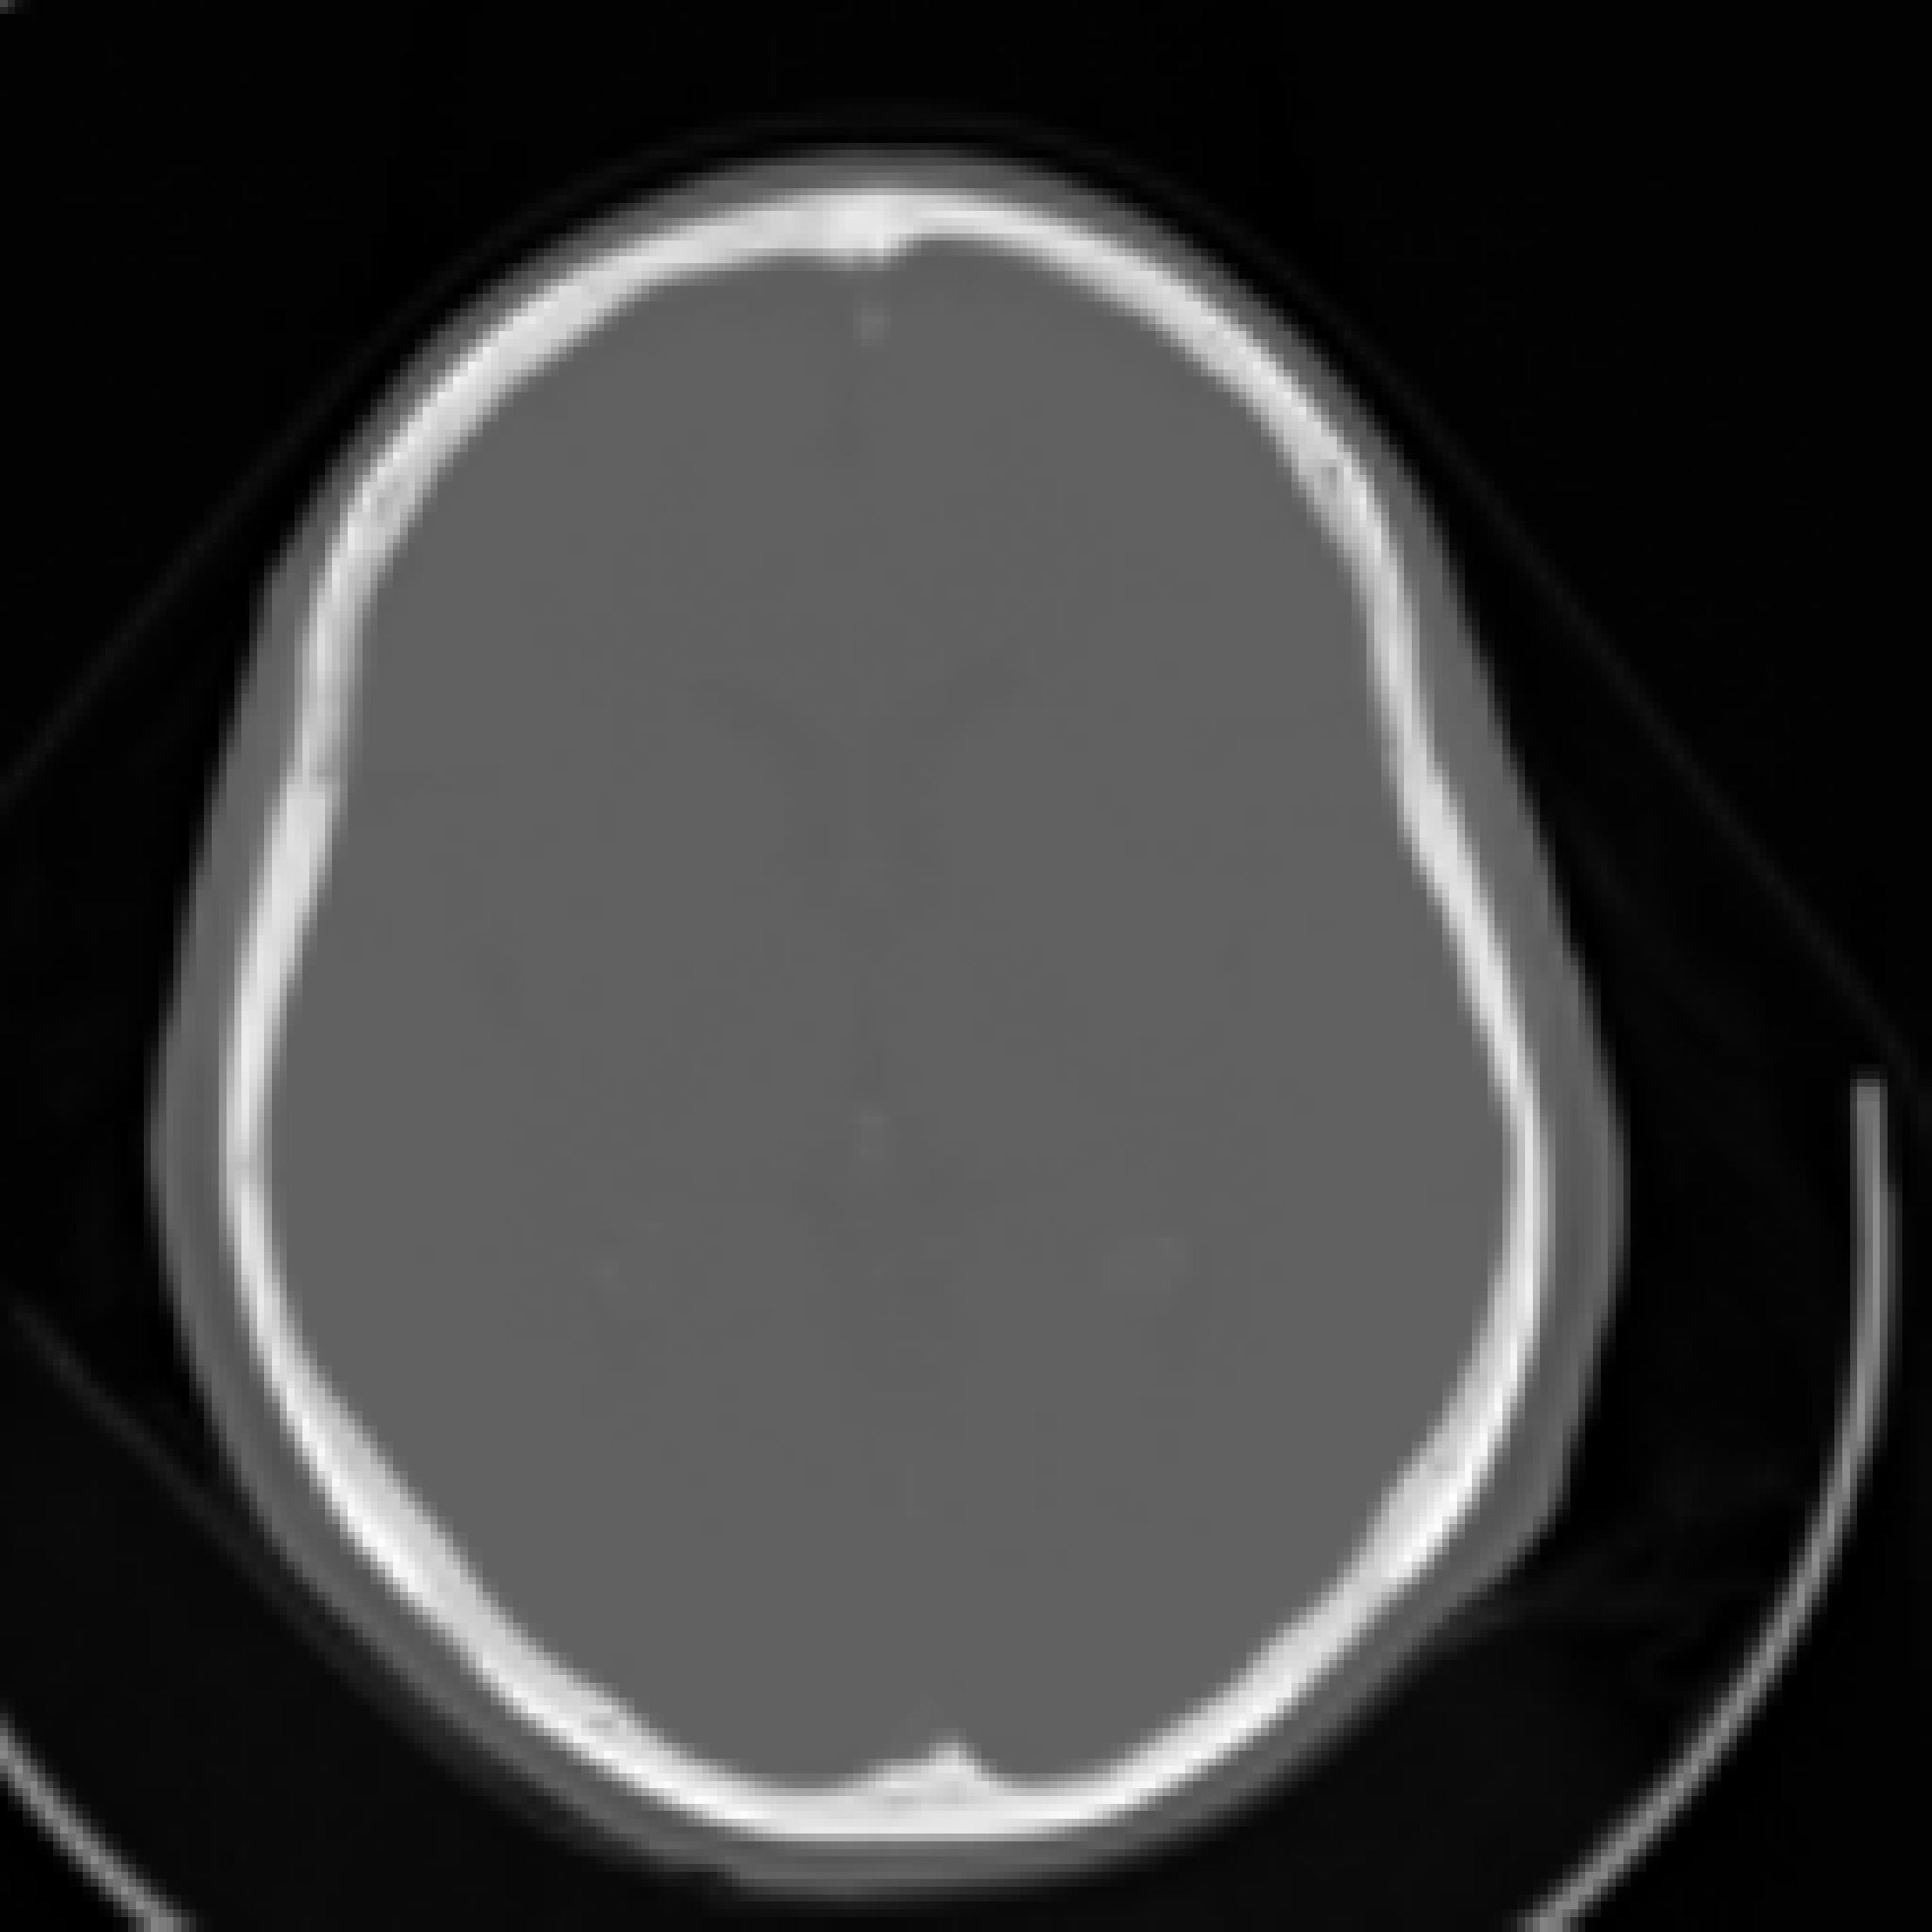
\includegraphics[width=\textwidth]{Figuras/Interpolate_bilinear_f=2.png}
            \caption{$256\times256$} 
         \end{subfigure}
         \begin{subfigure}[h]{0.24\textwidth}
            \centering
            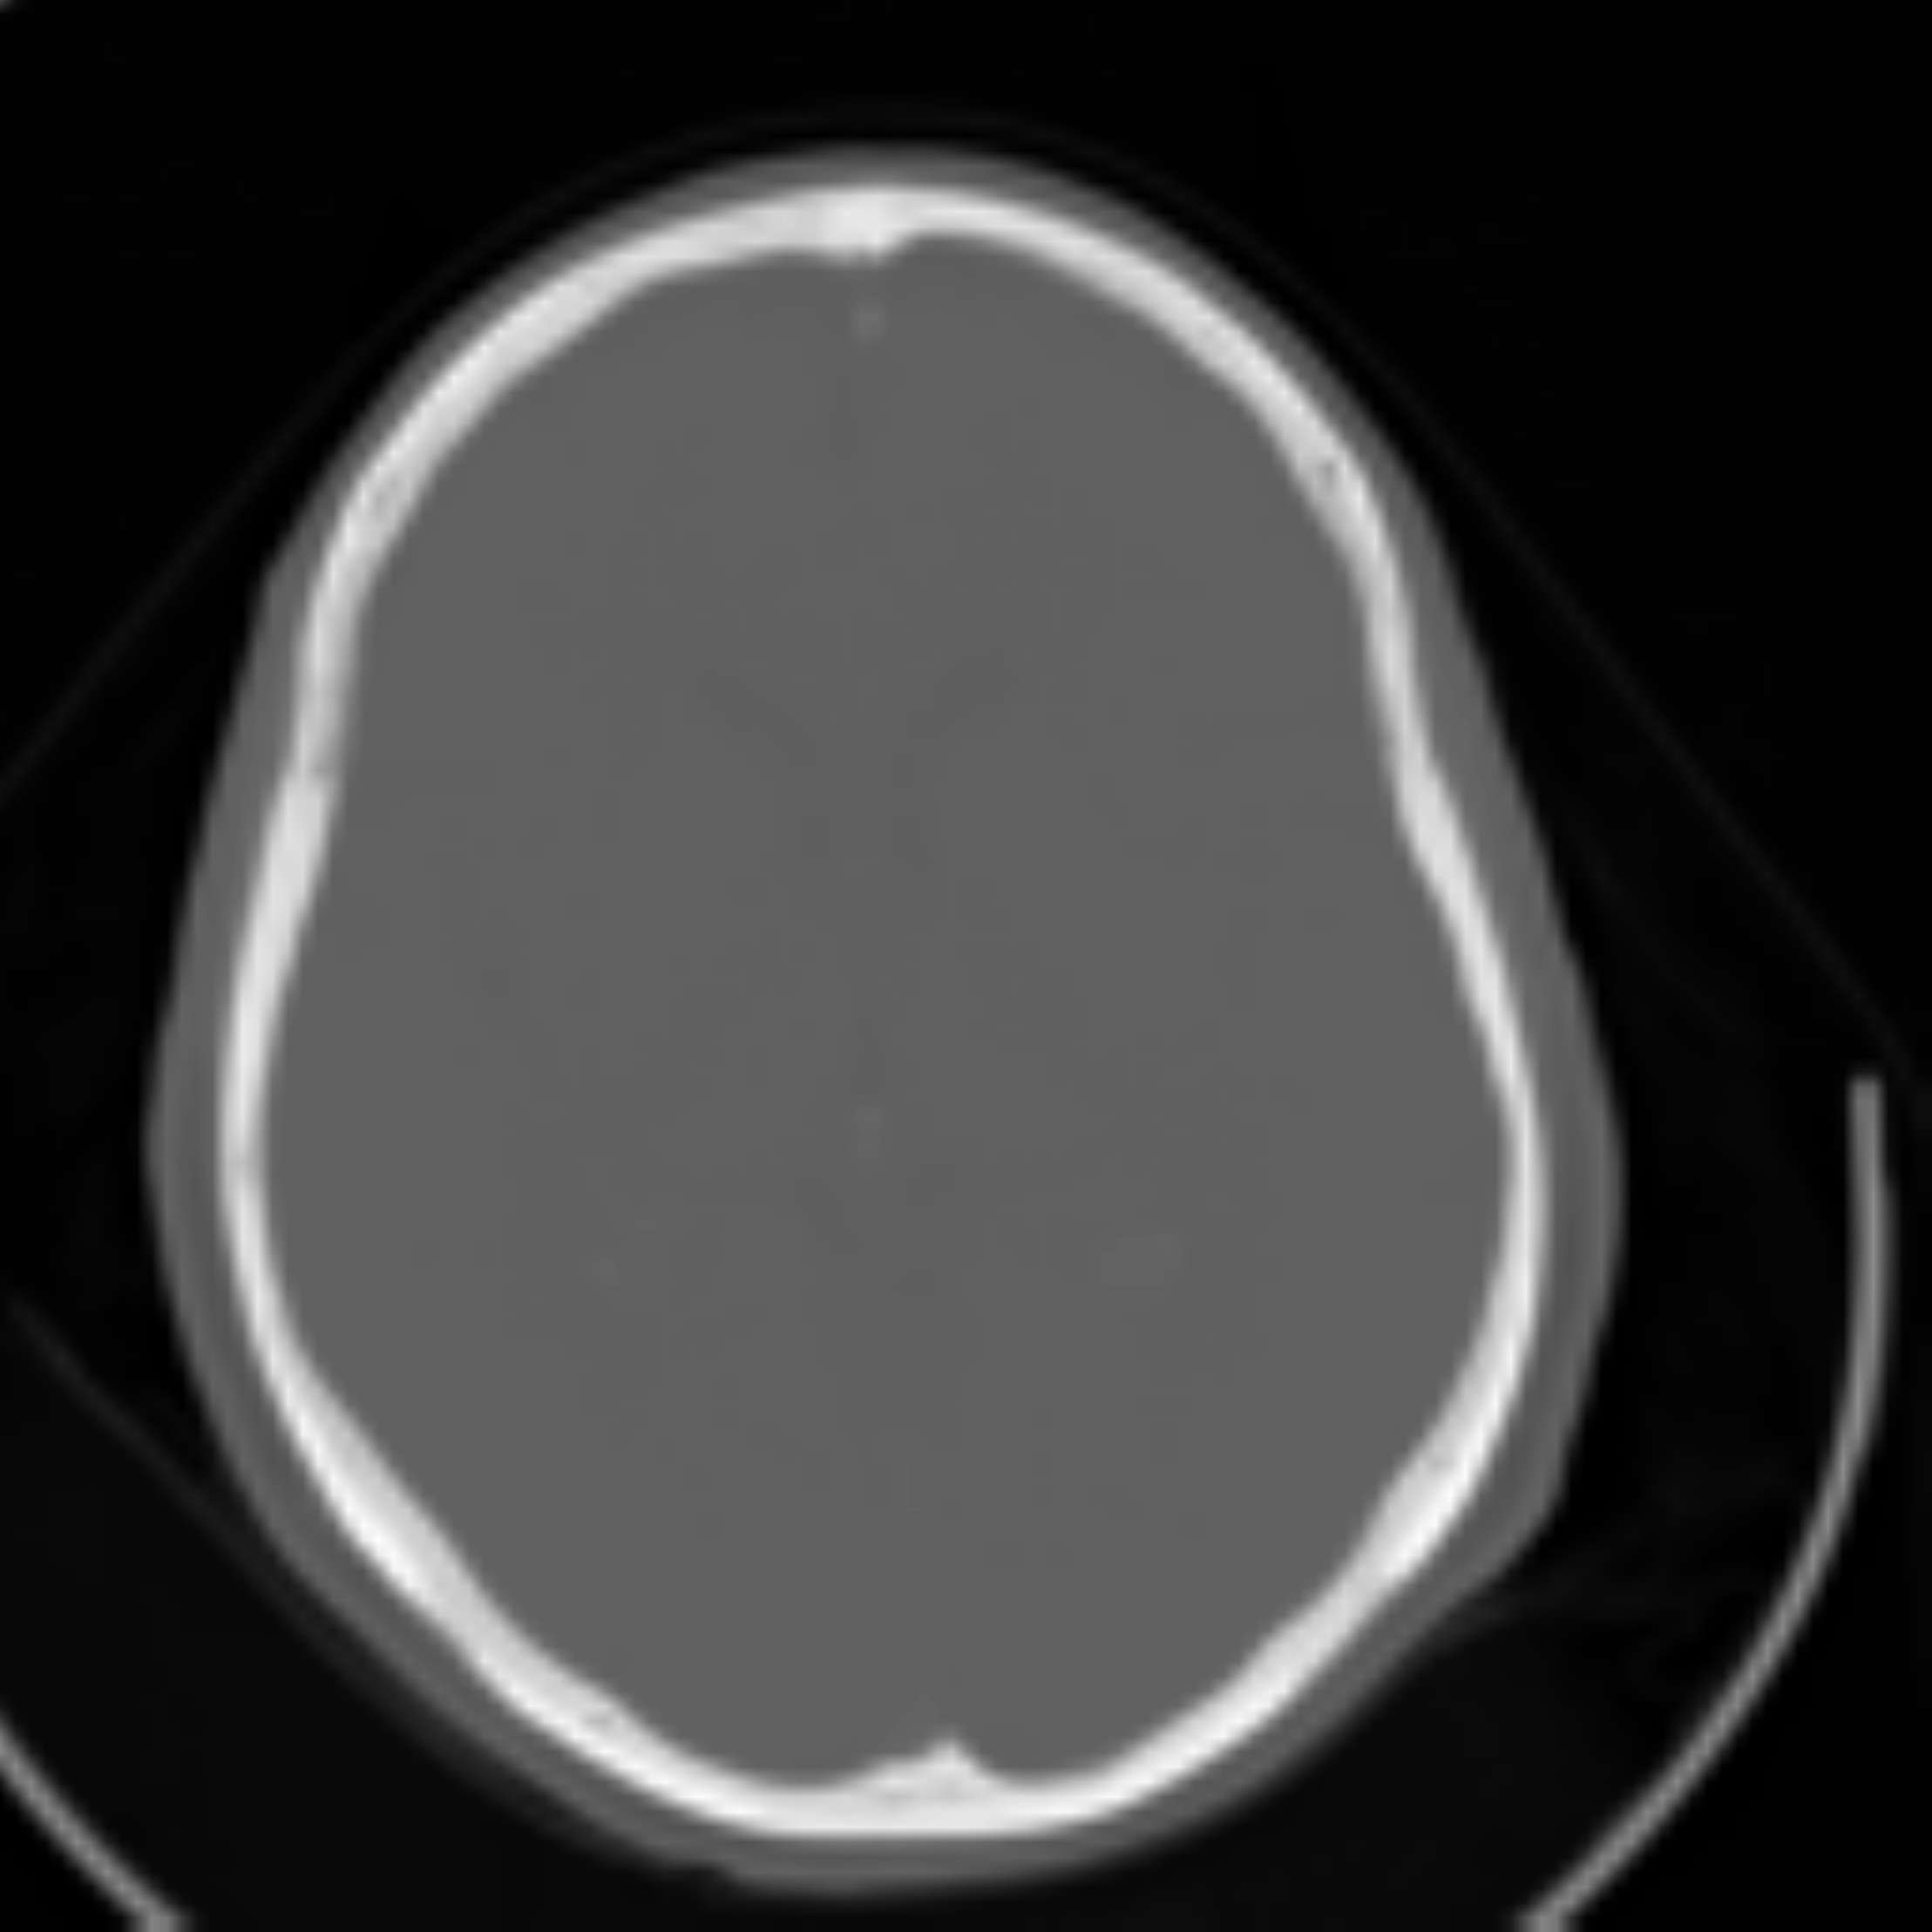
\includegraphics[width=\textwidth]{Figuras/Interpolate_bilinear_f=8.png}
            \caption{$1024\times1024$} 
         \end{subfigure}
    \caption{Distintos reescaleos de la imagen C con interpolación por los métodos de vecinos más cercanos (arriba) y bilineal (abajo).}
    \label{fig:Interpolate}
\end{figure}

\section{Filtros en el dominio espacial\label{sec:ej4}}

\vspace{0.3cm}

Se aplicaron filtros promedios pasabajos a las imágenes A y C con kernels de $3\times3$, $5\times5$ y $7\times7$ como se muestra en la Fig. \ref{fig:Pasabajo} utilizando $\verb|ImageJ|$. Estos filtros se definen a partir de kernels de la forma 
\begin{equation}
    h = \frac{1}{n^2} 
    \begin{bmatrix}
    1 & \cdots & 1 \\
    \vdots & \ddots & \vdots \\
    1 & \cdots & 1 \\
    \end{bmatrix}
\end{equation}
donde $n$ es la dimensión de la matriz. 

Se observa que a medida que se aumenta la dimensión del kernel, la imagen se vuelve cada vez más borrosa, es decir, el suavizado es mayor.

\begin{figure}[H]
    \centering
         \begin{subfigure}[h]{0.24\linewidth}
            \centering
            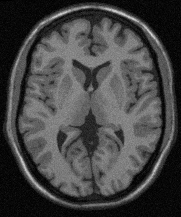
\includegraphics[width=\textwidth]{Figuras/ImagenA.png}
            \caption{Imagen A original} 
         \end{subfigure}
         \begin{subfigure}[h]{0.24\linewidth}
            \centering
            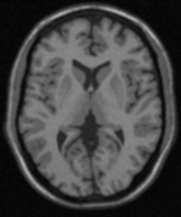
\includegraphics[width=\textwidth]{Figuras/ImagenA3x3.png}
            \caption{\centering Filtro \centering $3\times3$} 
         \end{subfigure}
         \begin{subfigure}[h]{0.24\linewidth}
            \centering
            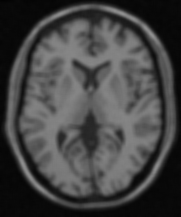
\includegraphics[width=\textwidth]{Figuras/ImagenA5x5.png}
            \caption{\centering Filtro $5\times5$} 
         \end{subfigure}
         \begin{subfigure}[h]{0.24\linewidth}
            \centering
            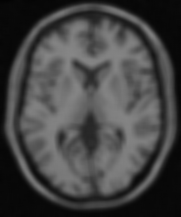
\includegraphics[width=\textwidth]{Figuras/ImagenA7x7.png}
            \caption{\centering Filtro $7\times7$} 
         \end{subfigure}
         \begin{subfigure}[h]{0.24\linewidth}
            \centering
            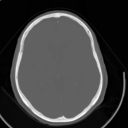
\includegraphics[width=\textwidth]{Figuras/ImagenC.png}
            \caption{Imagen C original} 
         \end{subfigure}
         \begin{subfigure}[h]{0.24\linewidth}
            \centering
            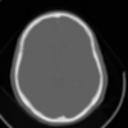
\includegraphics[width=\textwidth]{Figuras/ImagenC3x3.png}
            \caption{\centering Filtro $3\times3$} 
         \end{subfigure}
         \begin{subfigure}[h]{0.24\linewidth}
            \centering
            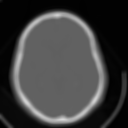
\includegraphics[width=\textwidth]{Figuras/ImagenC5x5.png}
            \caption{\centering Filtro $5\times5$} 
         \end{subfigure}
         \begin{subfigure}[h]{0.24\linewidth}
            \centering
            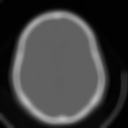
\includegraphics[width=\textwidth]{Figuras/ImagenC7x7.png}
            \caption{\centering Filtro $7\times7$} 
         \end{subfigure}
    \caption{Filtros promedios pasabajos aplicados a la imagen A (arriba) y a la imagen C (abajo) para distintas dimensiones de kernels.}
    \label{fig:Pasabajo}
\end{figure}


\section{Filtros en el dominio de frecuencias\label{sec:ej5}}

\vspace{0.3cm}

Dada una figura con componentes periodicas en su textura como la que se muestra en la Fig. \ref{fig:supermana}, es posible eliminar dichas componentes a partir de un procesamiento en el espacio de frecuencias de dicha imagen. Para esto se calcula la transformada de Fourier rápida (FFT por sus siglas en inglés) de la imagen con $\verb|ImageJ|$ y luego de reconocer las componentes periodicas, que en el espacio de frecuencias se manifiestan como puntos de alta intensidad, se procede a eliminarlas. Una vez eliminadas estas componentes se antitransforma la imagen (inverse FFT) y se recupera la imagen original con las componentes periodicas eliminadas. En la Fig. \ref{fig:superman} se muestra la imagen original (a) y la imagen procesada (b), mientras que en la Fig. \ref{fig:supermanfft} se muestra el espacio de frecuencias con la transformada de Fourier de la imagen original (a) y la transformada de Fourier con las componentes periodicas eliminadas (b). 

\begin{figure}[H]
    \centering
         \begin{subfigure}[h]{0.49\textwidth}
            \centering
            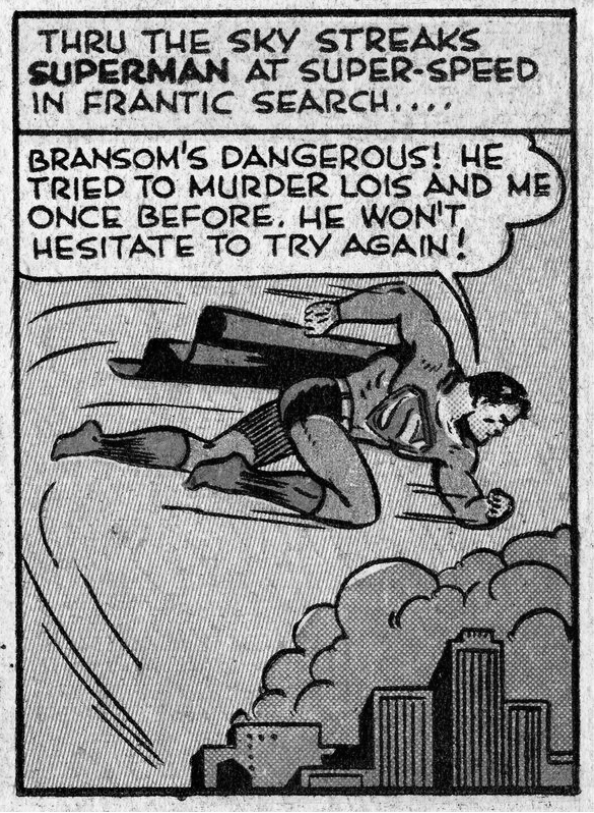
\includegraphics[width=0.75\textwidth]{Figuras/superman.png}
            \caption{Imagen original.} \label{fig:supermana}
         \end{subfigure}
         \begin{subfigure}[h]{0.49\textwidth}
            \centering
            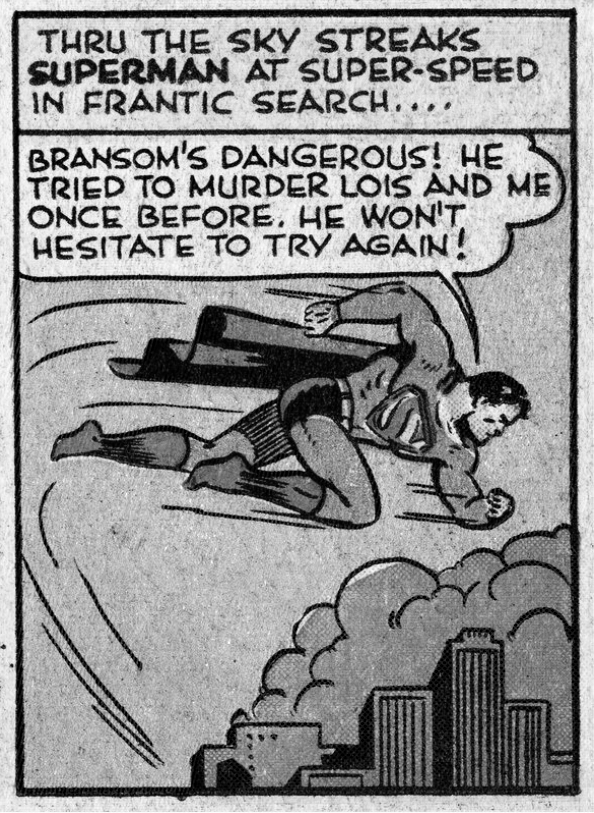
\includegraphics[width=0.75\textwidth]{Figuras/Inverse FFT of superman_process.png}
            \caption{Imagen procesada.}
         \end{subfigure}
    \caption{Comparación imagen original de Superman (a) con la imagen procesada (b) en el espacio de frecuencias sin las componentes periódicas en la textura.}
    \label{fig:superman}
\end{figure}


\begin{figure}[H]
    \centering
         \begin{subfigure}[h]{0.49\textwidth}
            \centering
            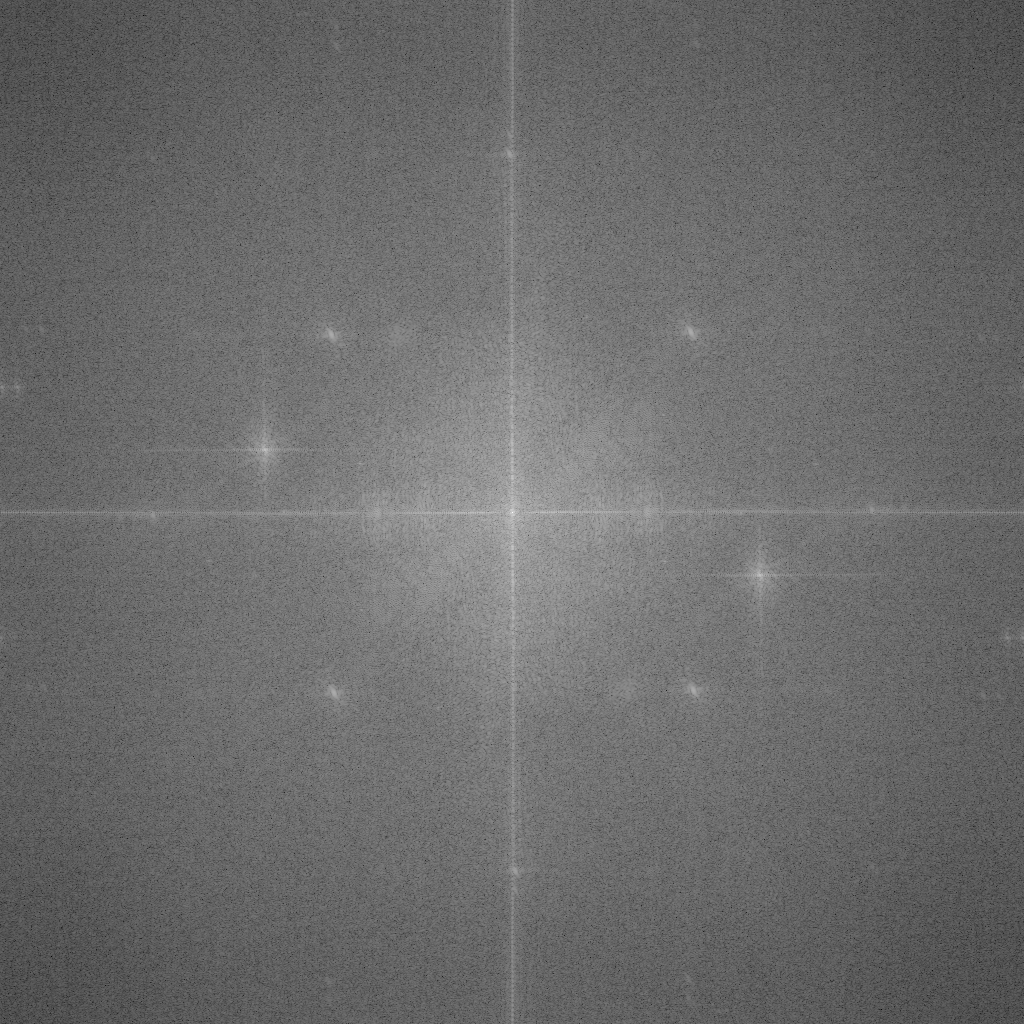
\includegraphics[width=0.75\textwidth]{Figuras/FFT of superman.png}
            \caption{FFT de Superman.} 
         \end{subfigure}
         \begin{subfigure}[h]{0.49\textwidth}
            \centering
            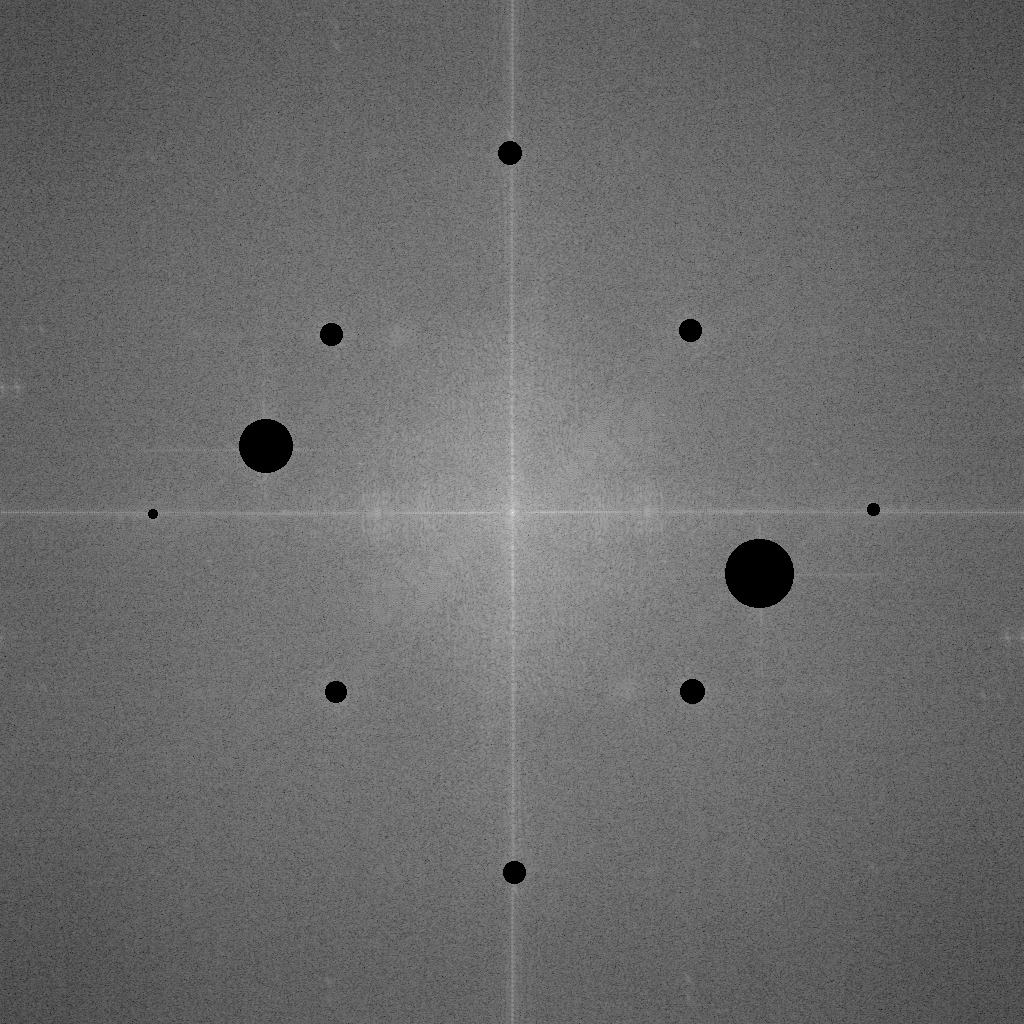
\includegraphics[width=0.75\textwidth]{Figuras/FFT of superman_process.png}
            \caption{FFT de superman procesada.}
         \end{subfigure}
    \caption{Transformada de Fourier rápida de Superman (a). Transformada de Fourier rápida sin las componentes periódicas. En el espacio de frecuencias las componentes periodicas se manifiestan como puntos de alta intensidad.}
    \label{fig:supermanfft}
\end{figure}

\section{Filtros Unsharp y Highboost\label{sec:ej6}}

\vspace{0.3cm}

Los filtros Unsharp y Highboost son filtros que se utilizan para resaltar los bordes de una imagen. Se definen de la siguiente manera: Sea $f(x,y)$ la imagen original con ruido, $\tilde{f}(x,y)$ la imagen original luego de aplicarle un filtro pasabajos y $g(x,y)$ la imagen resultante, entonces los filtros se definen como
\begin{itemize}
    \item Unsharp: $g(x,y) = f(x,y) - \tilde{f}(x,y)$
    \item Highboost: $g(x,y) = A~f(x,y) - \tilde{f}(x,y)$
\end{itemize}
donde $A$ es la intensidad del filtro High-boost y para $A=1$ el filtro High-boost es equivalente al filtro Unsharp. 

Se tomó la $\verb|imagenA.pgm|$ y se le agregó ruido gaussiano con desvio estándar $\sigma = 5$. Luego, se aplicaron los filtros Unsharp y Highboost utilizando un filtro pasa bajo promedio con un kernel de $7\times7$. Los resultados se muestran en la Fig. \ref{fig:highunsharp}. Se observa que ambos filtros resaltan los bordes de la imagen y amplifican el ruido, lo cual es esperable para este tipo de filtro que escencialmente se comportan como pasa altos. Se puede ver que el filtro Highboost con $A=2$ resalta los bordes, conservando mejor la imagen original. 

\begin{figure}[H]
   \centering
        \begin{subfigure}[h]{0.2\textwidth}
           \centering
           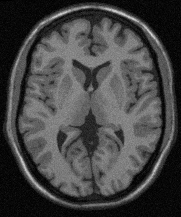
\includegraphics[width=\textwidth]{Figuras/ImagenA.png}
           \caption{Imagen A Original.} 
        \end{subfigure}
        \begin{subfigure}[h]{0.2\textwidth}
           \centering
           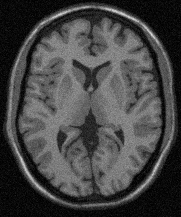
\includegraphics[width=\textwidth]{Figuras/ImagenA_noise=5.png}
           \caption{Imagen A con ruido.} 
        \end{subfigure}
        \begin{subfigure}[h]{0.2\textwidth}
           \centering
           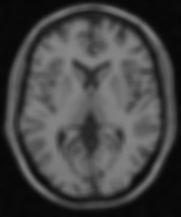
\includegraphics[width=\textwidth]{Figuras/ImagenA_noise=5_filter_7x7.png}
           \caption{Imagen A con ruido filtrada.} 
        \end{subfigure}
        \\
        \begin{subfigure}[h]{0.2\textwidth}
           \centering
           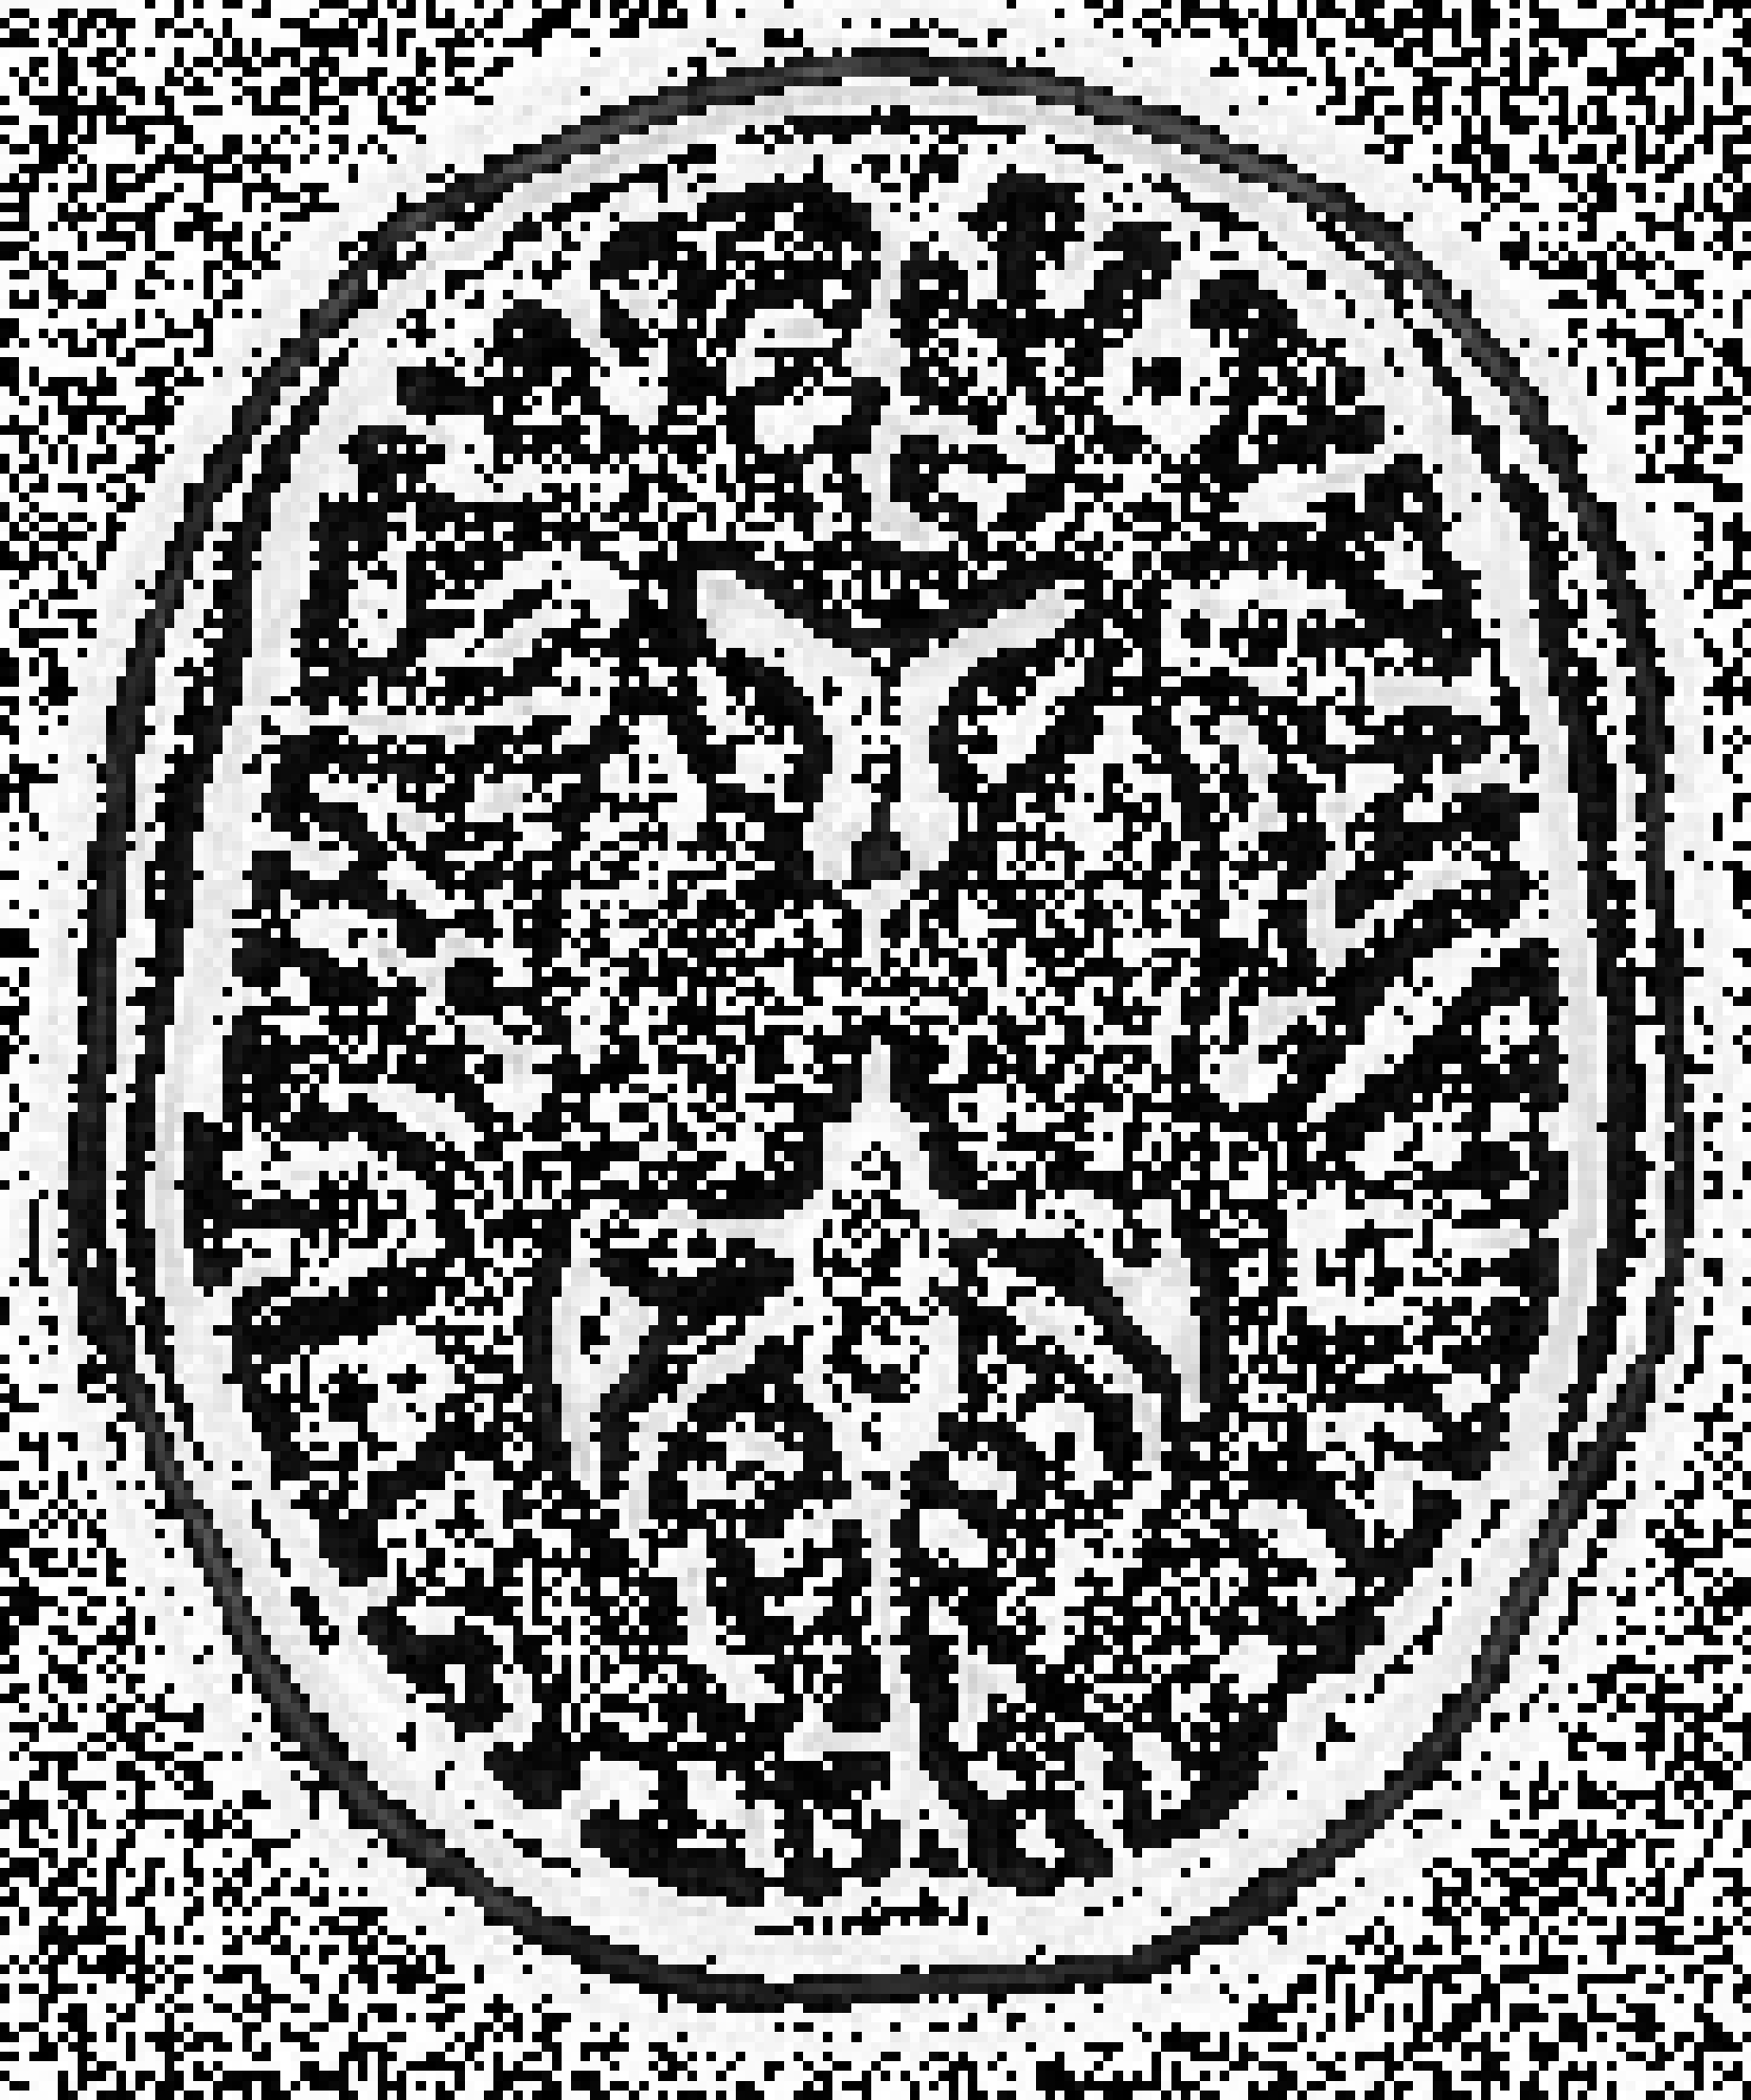
\includegraphics[width=\textwidth]{Figuras/unsharp.png}
           \caption{Filtro Unsharp.\\
           $~$} 
        \end{subfigure}
        \begin{subfigure}[h]{0.2\textwidth}
           \centering
           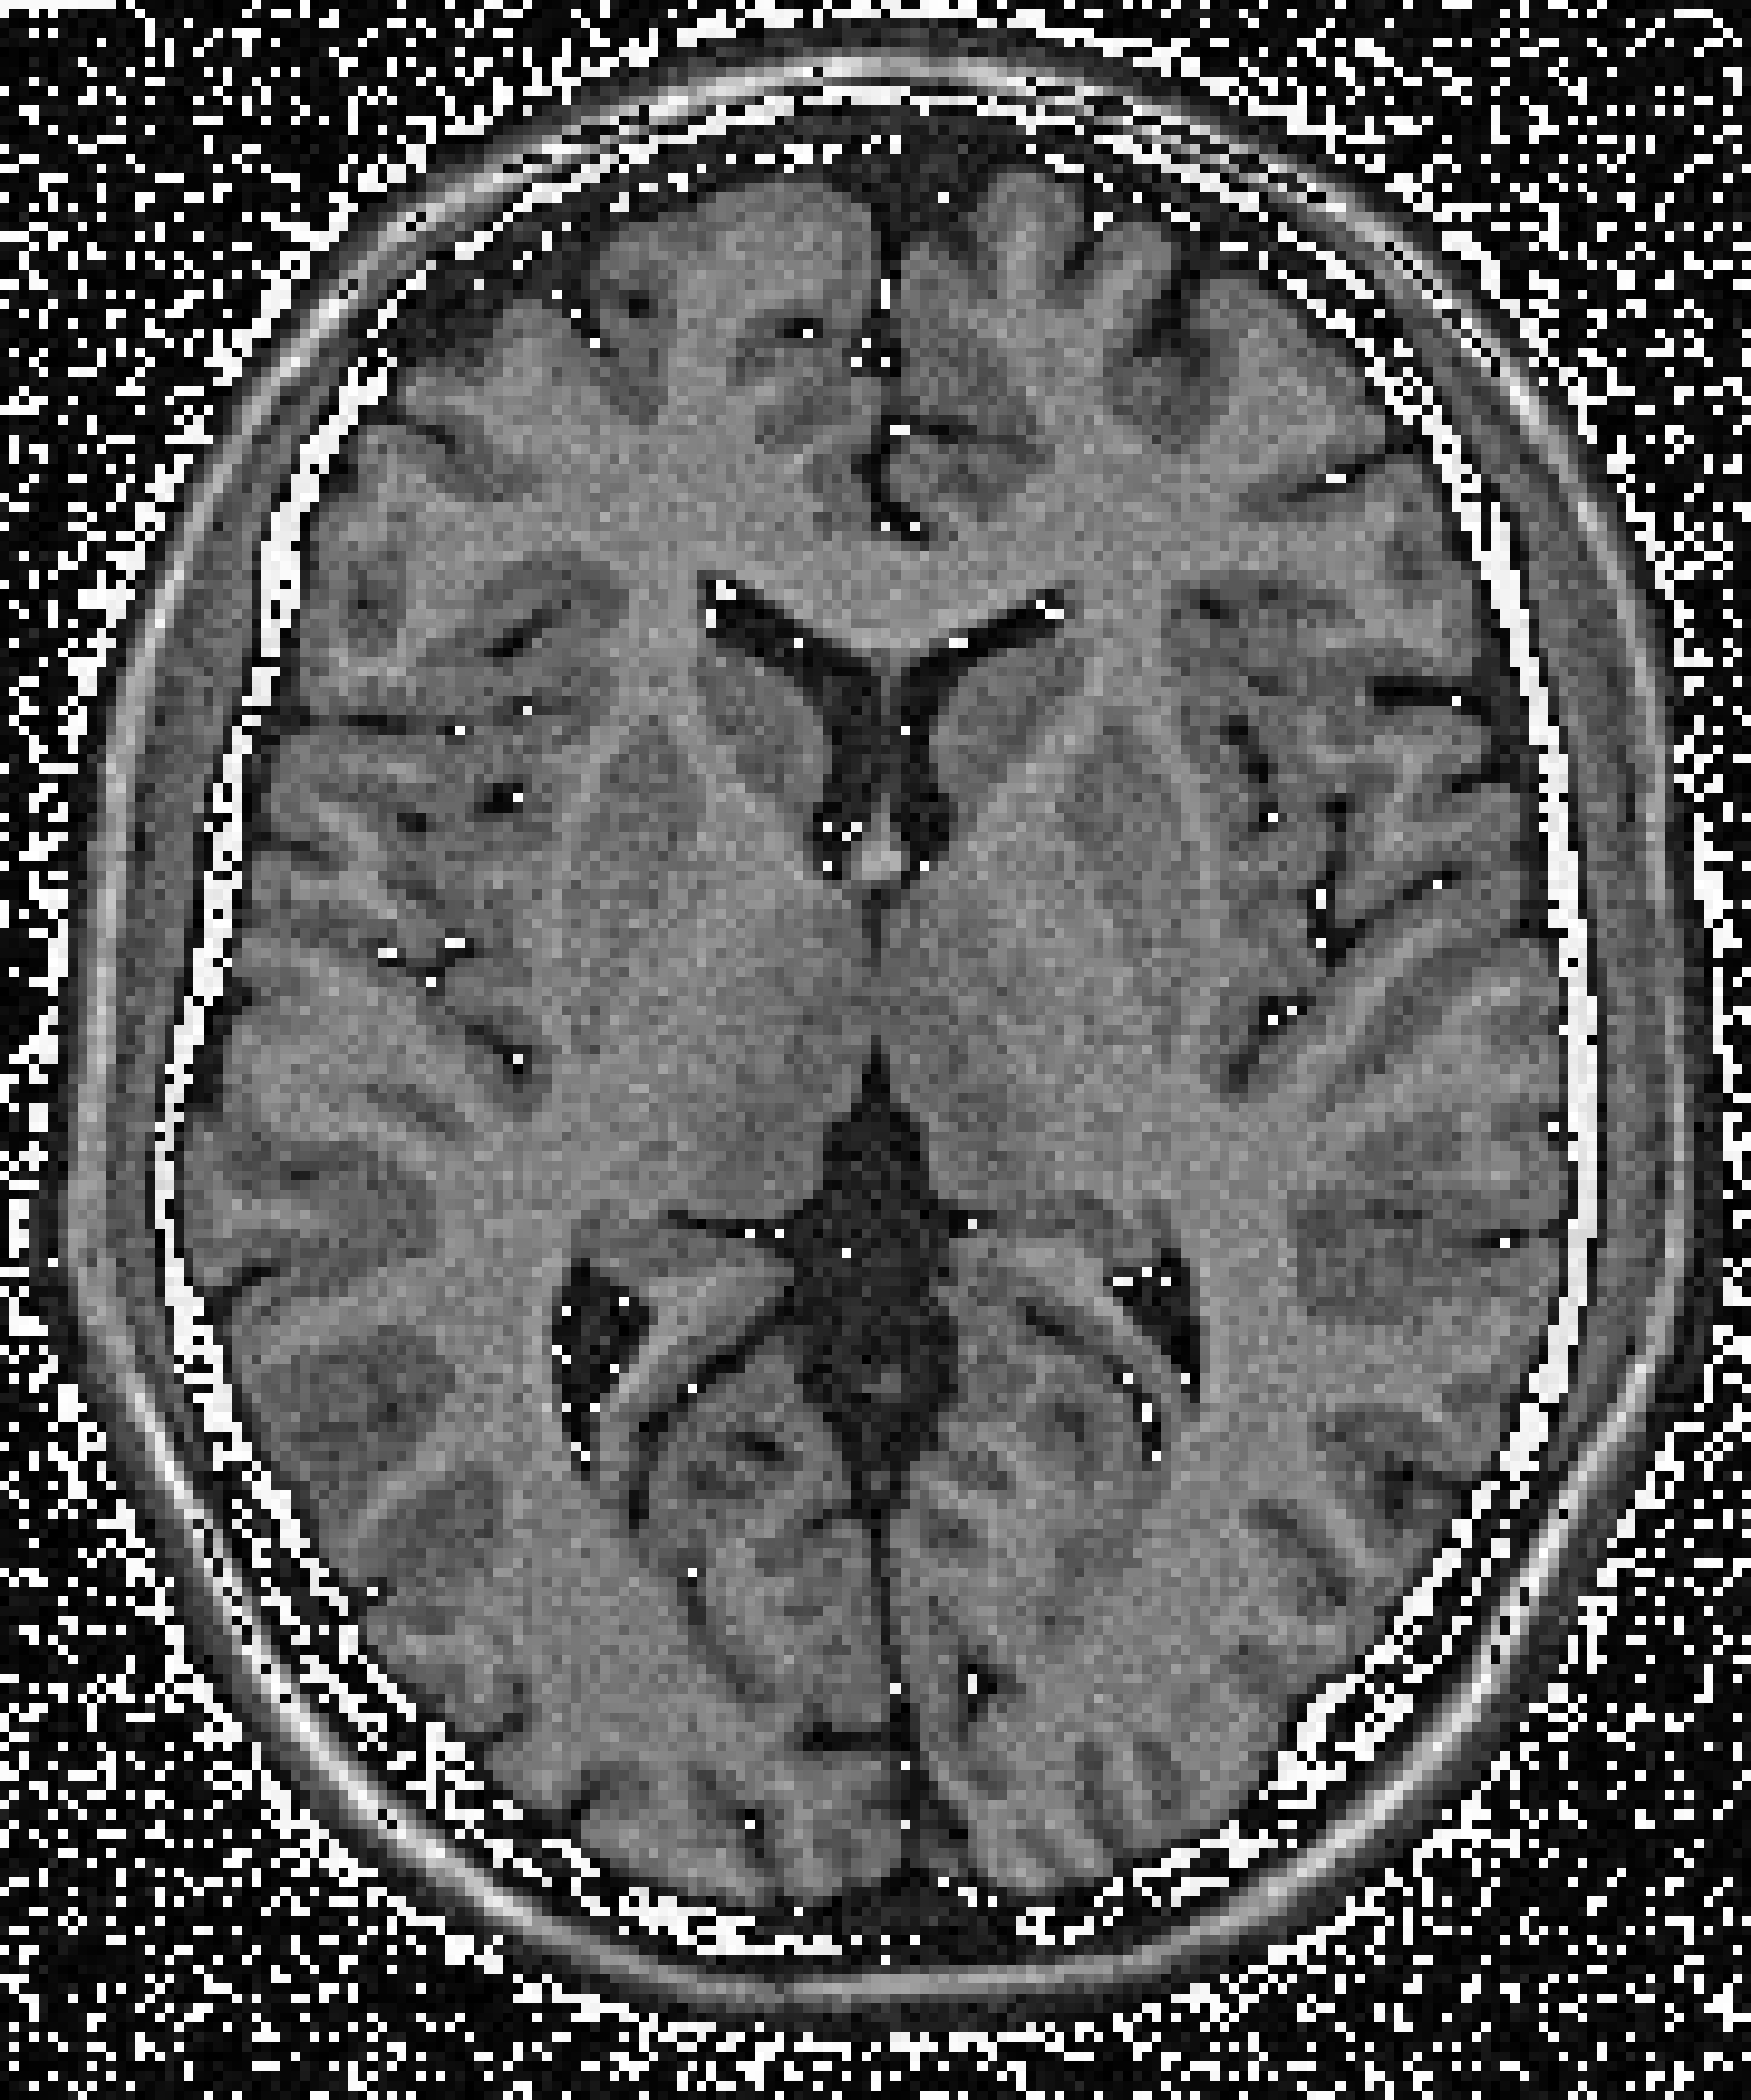
\includegraphics[width=\textwidth]{Figuras/highboost_A=2.png}
           \caption{Filtro Highboost con $A=2$.} 
        \end{subfigure}
        \begin{subfigure}[h]{0.2\textwidth}
           \centering
           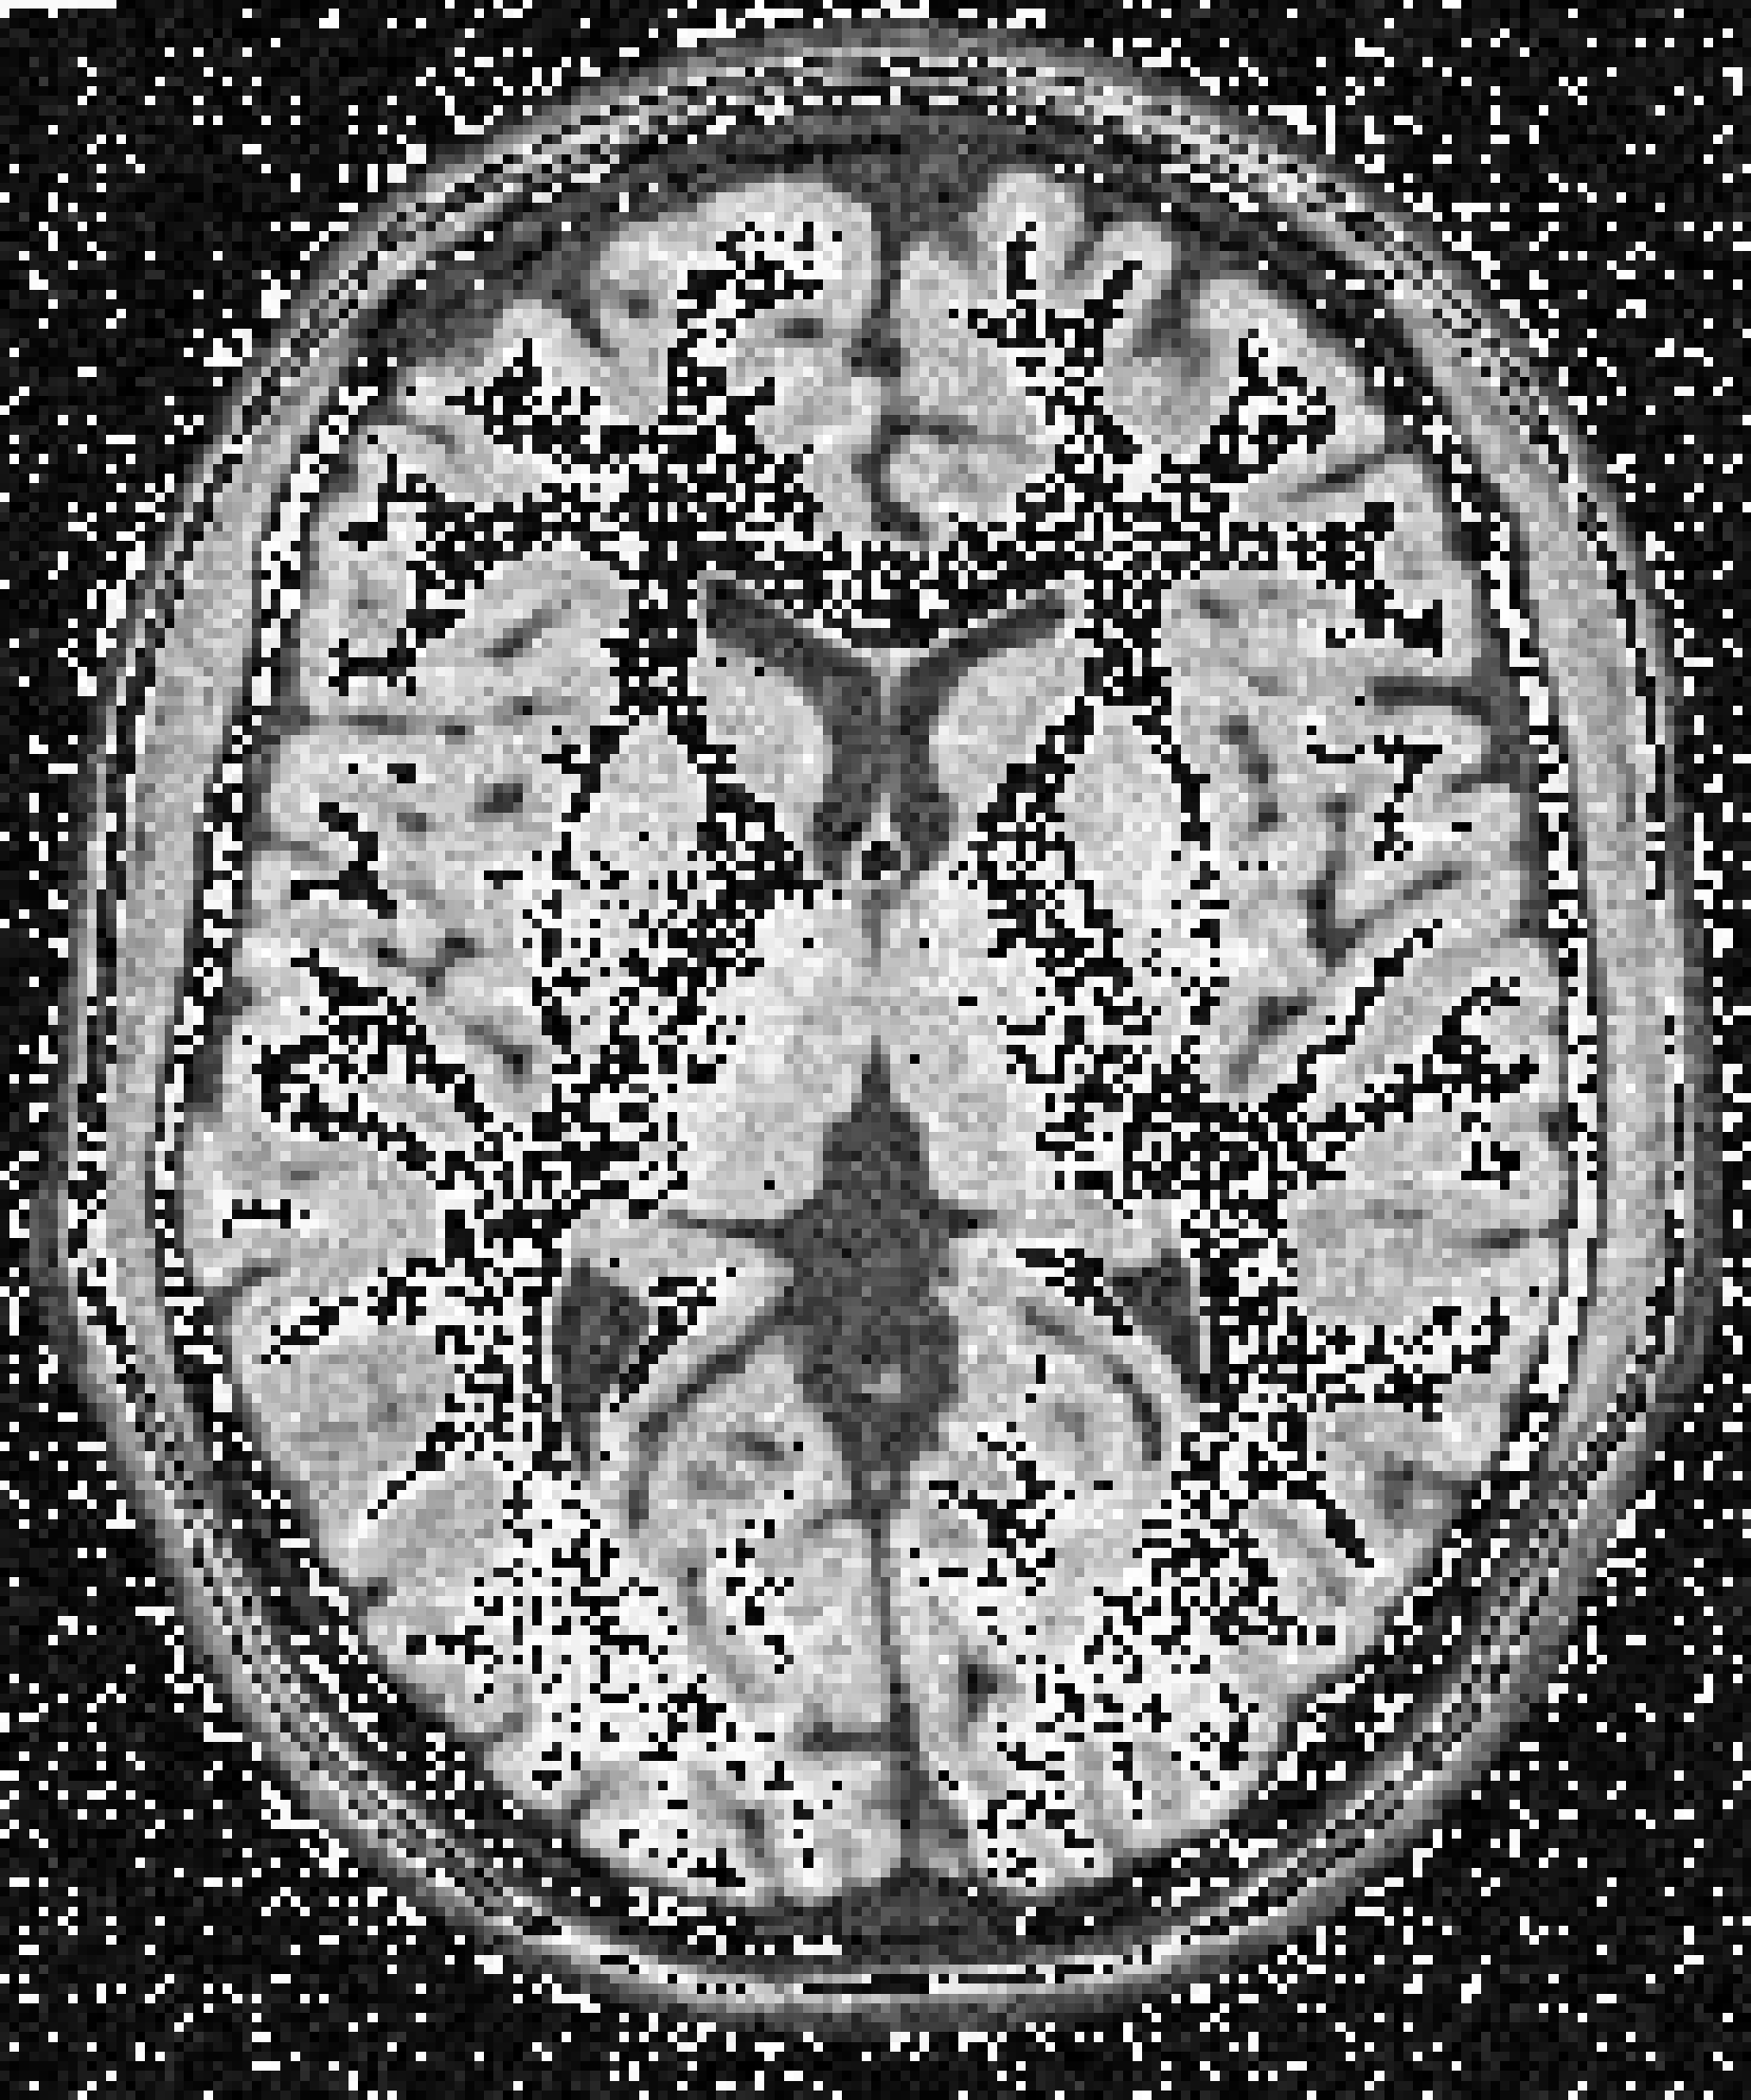
\includegraphics[width=\textwidth]{Figuras/highboost_A=3.png}
           \caption{Filtro Highboost con $A=3$.} 
        \end{subfigure}
   \caption{Filtros Unsharp y Highboost aplicados a la imagenA con ruido gaussiano con desvío estandar $\sigma =5$.}
   \label{fig:highunsharp}
\end{figure}

En la Fig. \ref{fig:plot_highboost} se grafica la media cuadrática de la resta entre la imagen con el filtro High-boost y la imagen original sin ruido en función de la intensidad del parámetro $A$. Se observa que $A=2$ es el valor óptimo para resaltar los bordes de la imagen alejandose lo menos posible (en media) de la imagen original.

\begin{figure}[H]
    \centering
         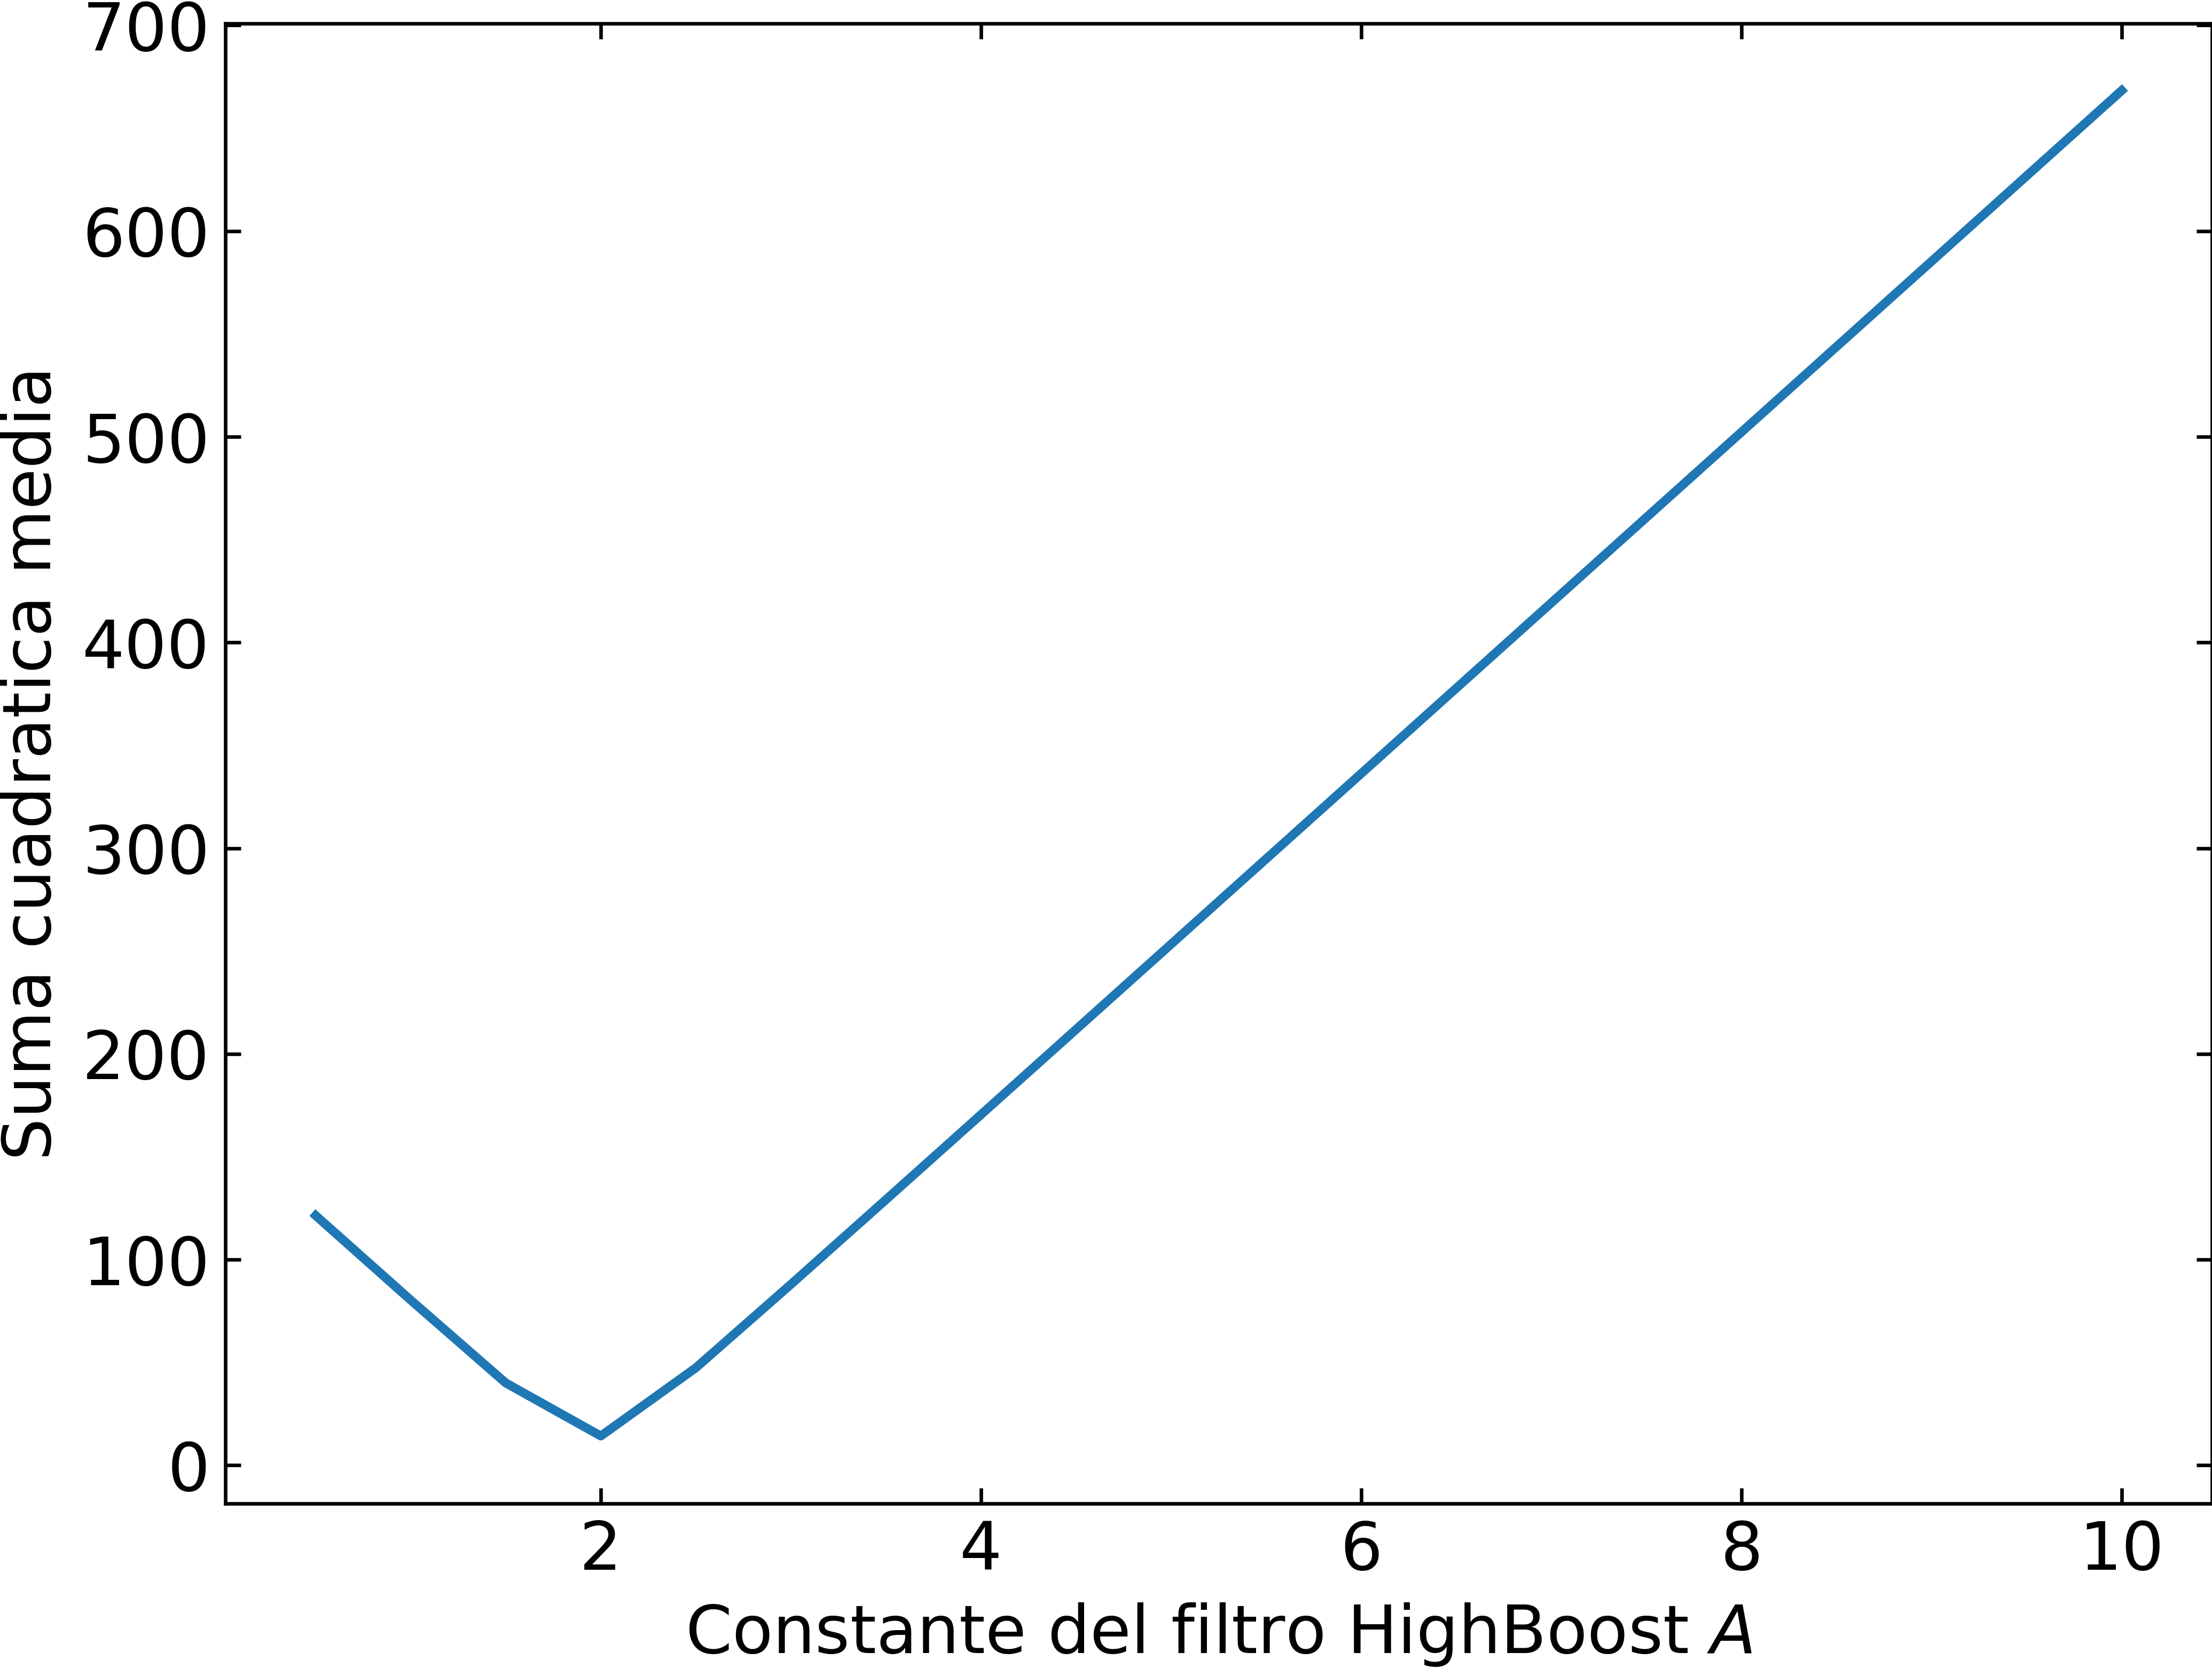
\includegraphics[width=0.6\textwidth]{Figuras/Highboost_plot.png}
    \caption{Gráfica de la media cuadrática de la diferencia entre la imagen original sin ruido y la imagen filtrada con el filtro High-boost en función del parámetro $A$.}
    \label{fig:plot_highboost}
\end{figure}

\section{Calibración de fantomas\label{sec:ej7}}

\vspace{0.3cm}

Se calcularon las relaciones señal-ruido (SNR) para los cortes 2, 3 y 4 de un fantoma adquiridos con CT HiSpeed. En este caso, se utilizó $\verb|ImageJ|$ para obtener los histogramas de intensidad de pixel en una región de interés (ROI por sus siglas en inglés) de los fantomas. Dichas ROI se tomaron como se muestra en la Fig. \ref{fig:SNR} para el caso de la imagen AAA0002 (cuadrado amarillo). La SNR se calcula como 
\begin{equation}
    SNR = \frac{\mu}{\sigma}
\end{equation}
donde $\mu$ es la media de la intensidad de la imagen y $\sigma$ es la desviación estándar en la ROI elegida. En la tabla \ref{tab:SNR} se muestran los valores de $\mu$, $\sigma$ y SNR para cada corte. Se observa que la SNR disminuye a medida que disminuye la corriente del tubo de rayos X. Esto es consistente con lo observado en las imágenes de los cortes, donde se observa que a menor corriente, la imágenes se vuelven más ruidosas.

\begin{figure}[H]
    \centering
         \begin{subfigure}[h]{0.49\linewidth}
            \centering
            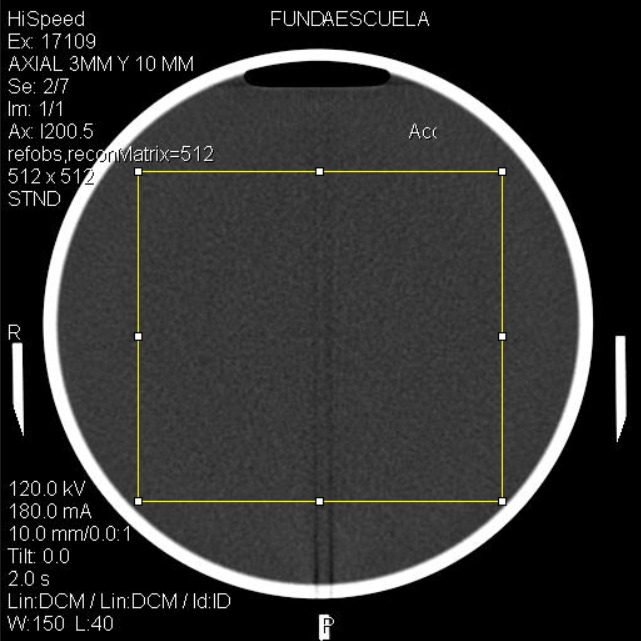
\includegraphics[width=0.7\textwidth]{Figuras/roi_corte2.png}
            \caption{Imagen con la ROI seleccionada  (cuadrado amarillo).} 
         \end{subfigure}
         \begin{subfigure}[h]{0.49\linewidth}
            \centering
            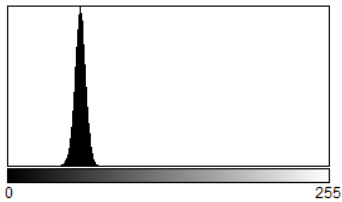
\includegraphics[width=\textwidth]{Figuras/hist_corte2.png}
            \caption{Histograma de intensidades.}
         \end{subfigure}
    \caption{Estimación de la SNR para la imagen AAA0002.}
    \label{fig:SNR}
\end{figure}

\begin{table}[H]
    \centering
    \begin{tabular}{c||c|c|c|c}
    \hline
    Corte & Corriente (mA) & $\mu$     & $\sigma$ & SNR \\ \hline
    2     & 180.0          & 57.074 & 4.422 & 12.907   \\ \hline
    3     & 100.0          & 56.722 & 5.769 & 9.832   \\ \hline
    4     & 60.0           & 56.728 & 7.286 & 7.786   \\ \hline
    \end{tabular}
    \caption{Tabla de corriente, media, desviación estándar y SNR para las imágenes AAA000x siendo x el corte.} \label{tab:SNR}
\end{table}

Por otro lado, se midió la \textit{point spread function} definida por el ancho total a media altura (FWHM por sus siglas en inglés) del perfil de intensidad del punto blanco del fantoma para los cortes 11, 12, 13 y 14. En la Fig. \ref{fig:FWHMa} se muestra la imagen AAA0011 y la ROI sobre el cual se obtuvo el perfil de intensidad (linea amarilla en la imagen inscrustada) y en la Fig. \ref{fig:FWHMb} se muestra el FWHM para dicho perfil de intensidad. En la tabla \ref{tab:FWHM} se muestran los valores de FWHM para cada corte. Se ve que la \textit{point spread function} es menor para la imagen AAA0012 con filtro EDGE.

\begin{table}[H]
    \centering
    \begin{tabular}{c||c|c}
    \hline
    Corte & Filtros & FWHM  \\ \hline
    11 & STND    & 5.720   \\ \hline
    12 & EDGE    & 2.967   \\ \hline
    13 & SOFT    & 6.267   \\ \hline
    14 & CHST    & 4.425   \\ \hline
    \end{tabular}
    \caption{Tabla de filtro y FWHM para las imágenes AAA00xx siendo x el corte.} 
    \label{tab:FWHM}
\end{table}

\begin{figure}[H]
    \centering
         \begin{subfigure}[h]{0.49\linewidth}
            \centering
            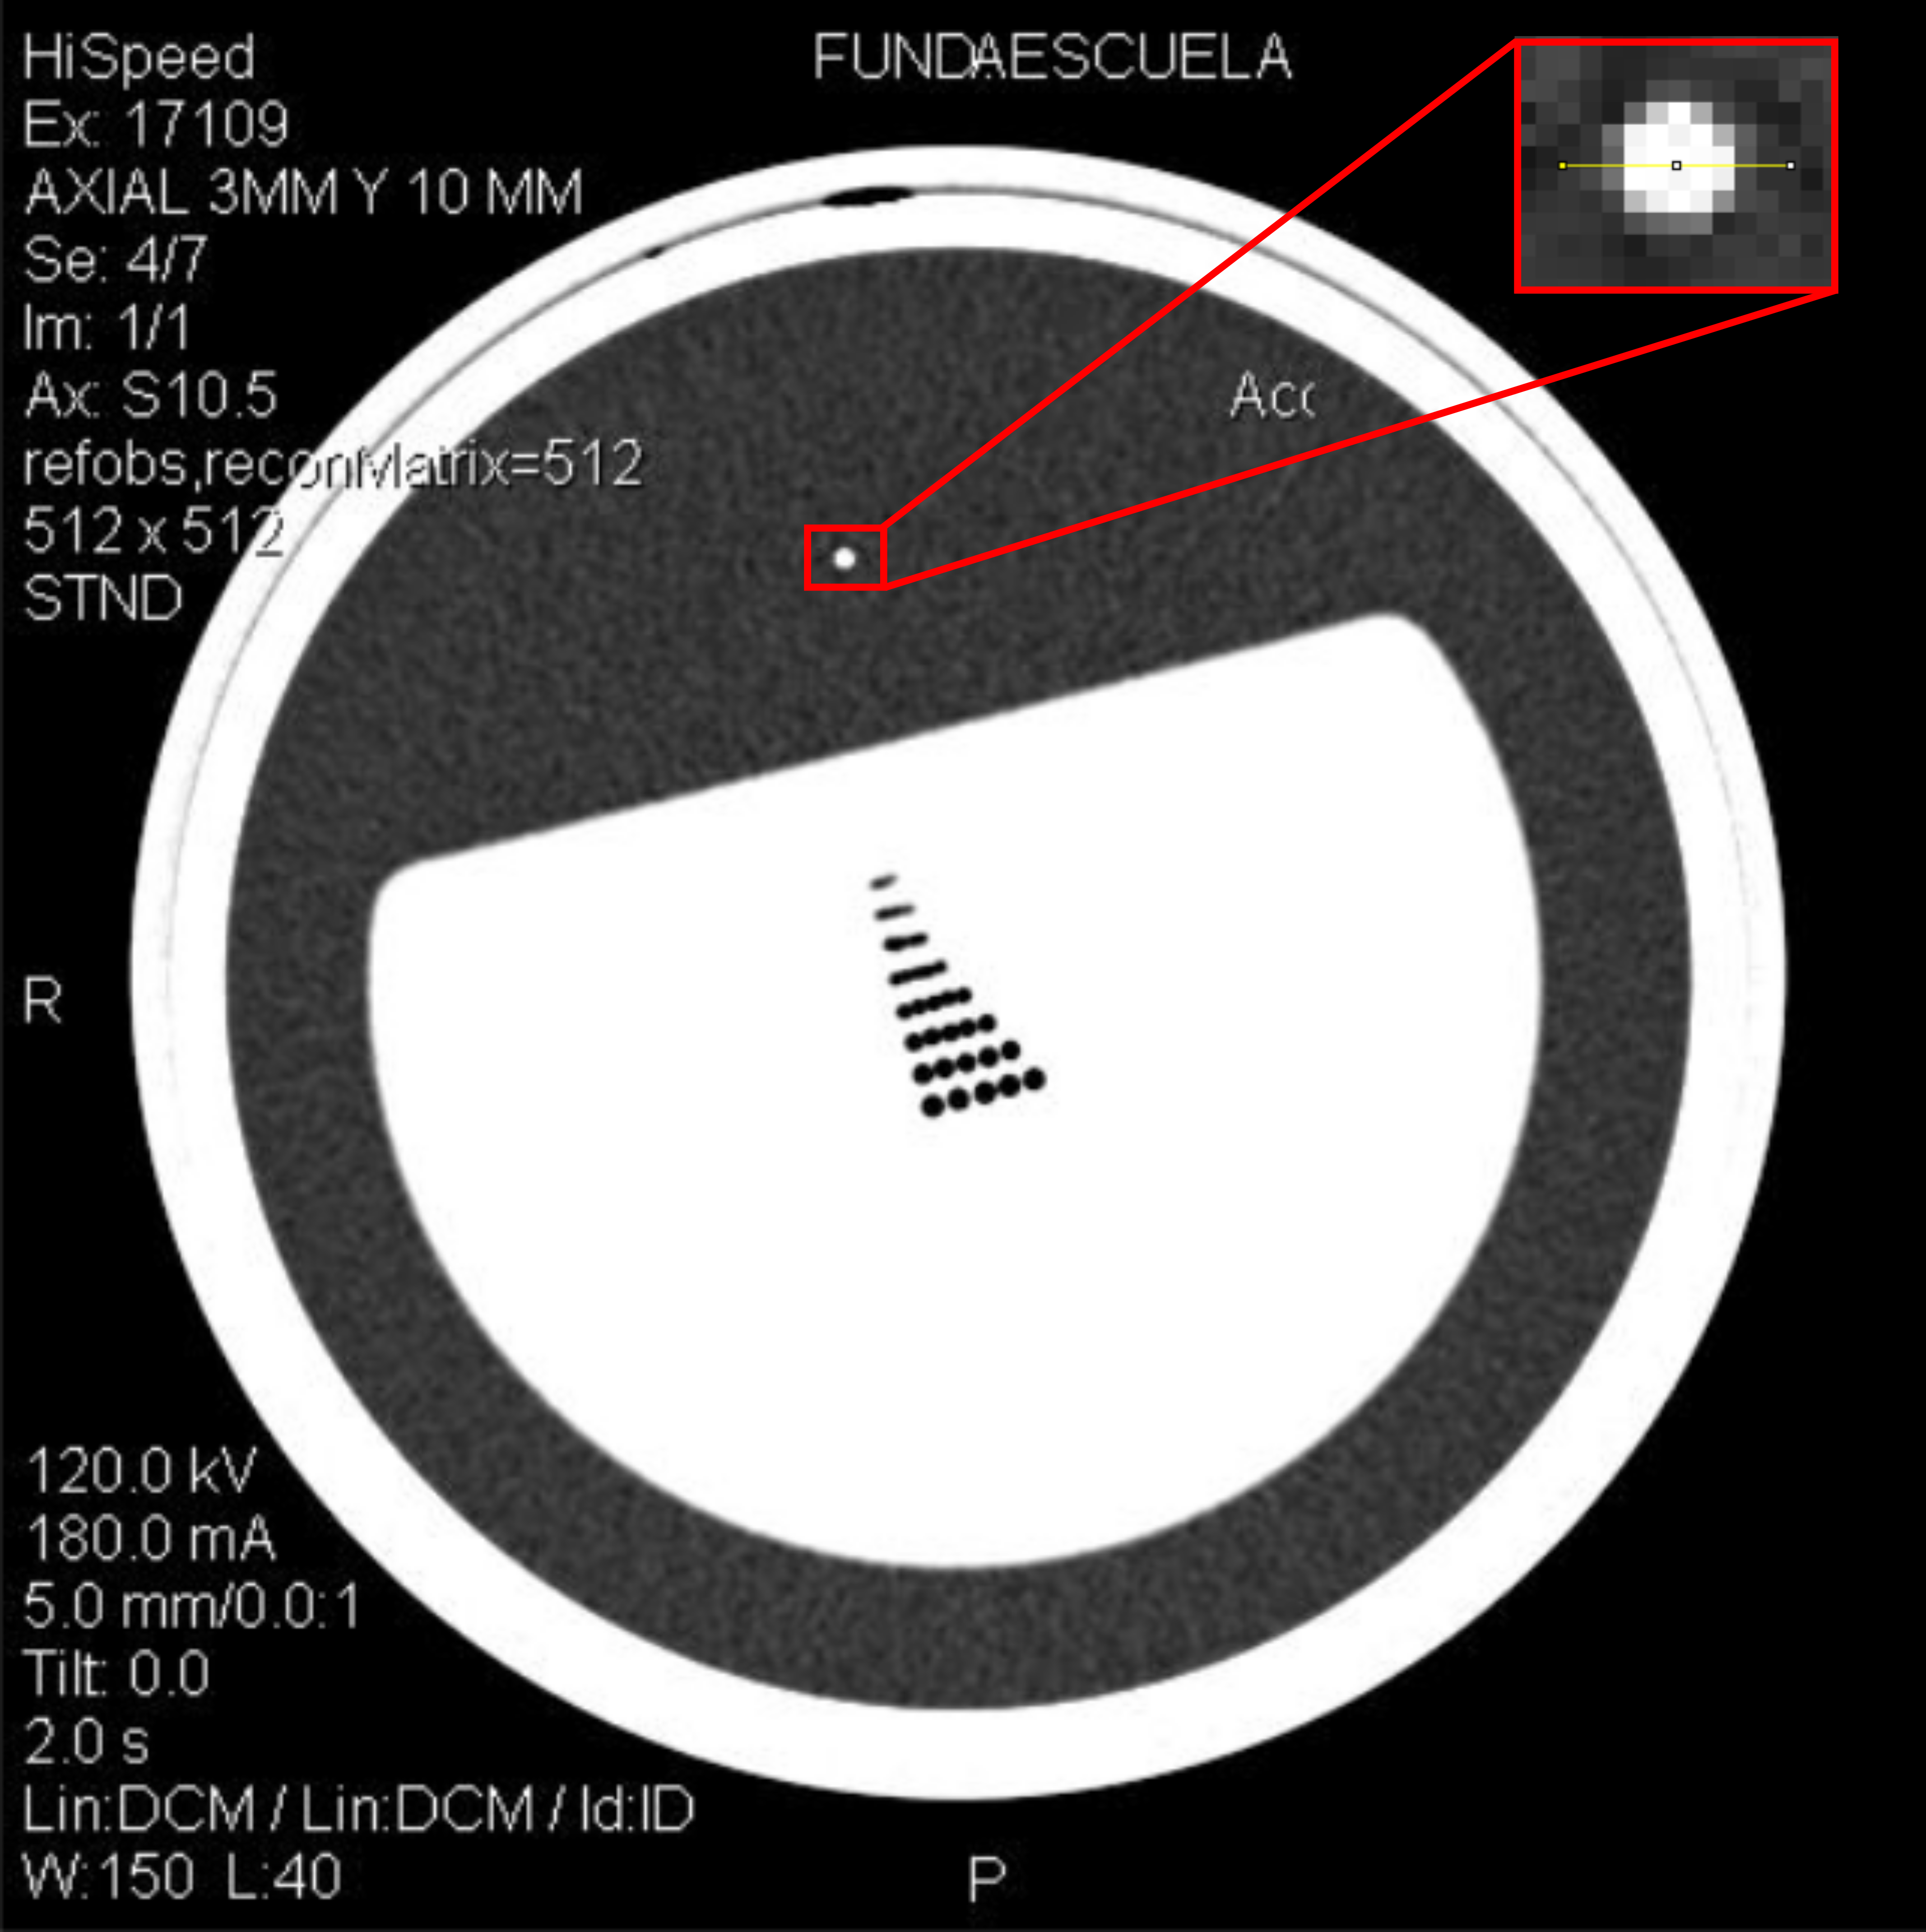
\includegraphics[width=0.7\textwidth]{Figuras/roi_zoom_corte11.png}
            \caption{Imagen con la ROI seleccionada (linea amarilla en la imagen inscrustada).}     \label{fig:FWHMa}
         \end{subfigure}
         \begin{subfigure}[h]{0.49\linewidth}
            \centering
            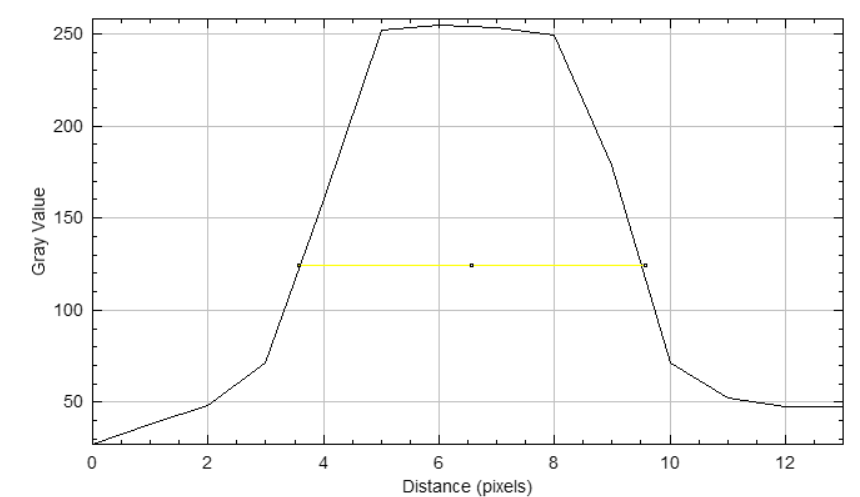
\includegraphics[width=\textwidth]{Figuras/profile_corte11.png}
            \caption{Perfil de intensidad.}\label{fig:FWHMb}
         \end{subfigure}
    \caption{Estimación del FWHM para la imagen AAA0011.}
    \label{fig:FWHM}
\end{figure}

%\begin{figure}[h]
%    \centering
%         \begin{subfigure}[h]{0.9\linewidth}
%            \centering
%            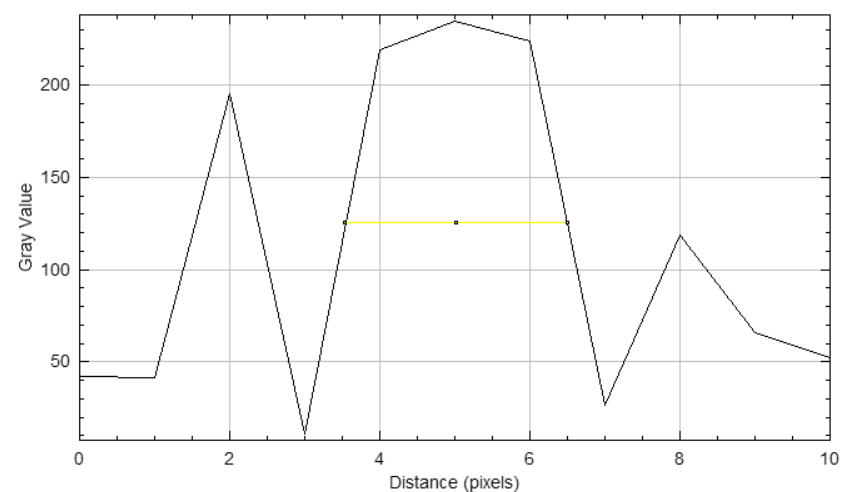
\includegraphics[width=\textwidth]{Figuras/profile_corte12.png}
%            \caption{ImagenA original junto con su histograma de intensidades.} 
%         \end{subfigure}
%    \caption{}
%    \label{fig:corte12}
%\end{figure}

\centerline{\rule{0.95\linewidth}{0.6pt}}


%\bibliographystyle{plain} % Estilo de bibliografía
%\bibliography{bibliography}    % Nombre de tu archivo .bib sin la extensión


\end{document}